\documentclass[12pt, a4paper]{article}
\usepackage{graphicx}
\usepackage[a4paper, total={6in, 8in}]{geometry}
\usepackage{setspace}
\usepackage{parskip}
\usepackage{float}
\usepackage{amsmath}
\usepackage{subfig}
\usepackage{xcolor}
\usepackage[numbered]{matlab-prettifier}

\begin{document}

\graphicspath{{./images}}

\begin{center}
    \onehalfspacing
    {\Large \textbf{King Fahd University of Petroleum and Minerals} }\\ 
    {\large \textbf{
    College of Computing and Mathematics\\
    Computer Engineering Department 
    } } 
\end{center} 

\begin{figure}[h]
    \centering
    
\includegraphics[width=200px]{images/KFUPM_LOGO.png}
\end{figure}

\begin{center}\onehalfspacing
    \large \textbf{COE 588- Modeling \& Simulation \\of computer and networks Systems }\\
    \normalsize \textbf{Term 232} \\
    \large \textbf{Progress Report}\\
    \textbf{Project}: Simulation and evaluation of M/M/c \\ with an infinite buffer 
\end{center}
\vspace{1em}
\large
\begin{center}
\bgroup
\def\arraystretch{1.3}
\begin{tabular}{|c|c|}
    \hline
    \textbf{Name} & \textbf{KFUPM ID} \\
    \hline
    Hashim Al-Sadah & 201578370\\
    \hline
    Abdulwahab Alghamdi & 201734070\\
    \hline
    Hussain Al-Sinan & 202205120\\
    \hline 
\end{tabular}
\egroup
\end{center}
\vspace{1em}
\begin{center}
    \textbf{Instructor:} Dr. Ashraf S. Hasan Mahmoud.
\end{center}
\normalsize


\onehalfspacing

\section{Objective}
To simulate the multiple servers queueing system with an infinite buffer, M/M/c, 
and verify that the simulation results match with the theoretical ones. 
The average total time, average waiting time, average number of customers in the system, 
average number of customers in the buffer, and the probability of waiting will 
be simulated as function of the traffic intensity. 
Additionally, the (Probability Density Function) PDF of the total time spent in the system, 
the PDF of the waiting time in the buffer, 
and the (Probability Mass Function) PMF of the number of customers in the system will 
be obtained empirically for low, medium, and high traffic intensity. Finally, we will 
study the effect of increasing the number of servers on the probability of waiting for a fixed
traffic intensity. All the results obtained through simulation will be compared against
the theoretical ones.

\section{Theoretical Background}
The state diagram for M/M/c is shown in Figure \ref{state_diagram_MMc}. The 
number of servers is denoted by $c$, the arrival rate is $\lambda$, and the 
service rate when the system at some state $s$ is $min(s\mu, c\mu)$.

\begin{figure}[H]
  \centering 
  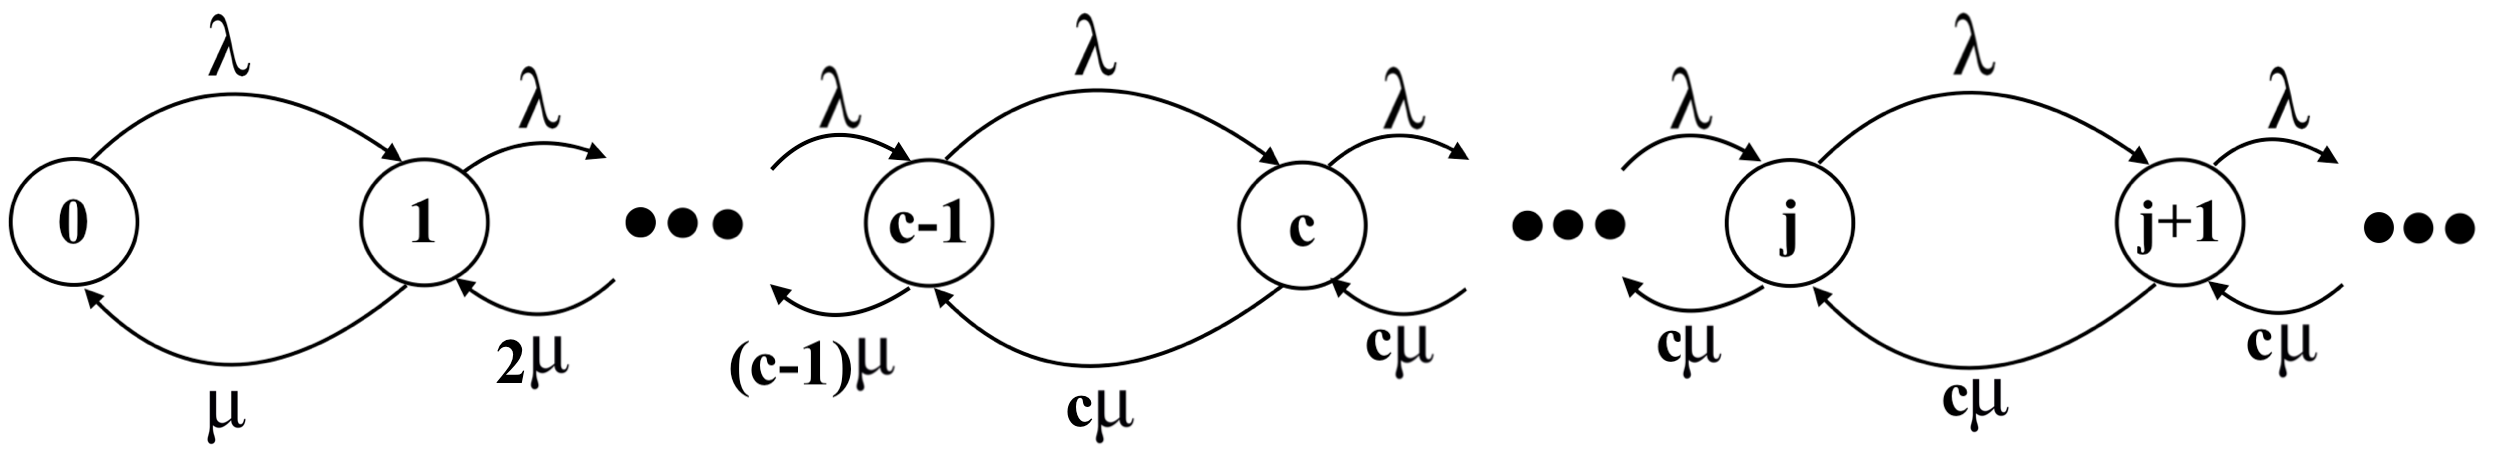
\includegraphics[width=430px]{images/MMc_state_diagram.png}
  \caption{State diagram of M/M/c}
  \label{state_diagram_MMc}
\end{figure}

From the state diagram, one can obtain the global equations and derive 
the equations that describe M/M/c. We will state the equations here without
derivation.

Define $a = \lambda / \mu$. Then the traffic intensity $\rho$ is 
\begin{equation}
  \rho = \frac{a}{c} = \frac{\lambda}{c \mu}
\end{equation}
For all the following equations, we assume that the system is stable. That is 
$\rho < 1$. Then the PMF of $N(t)$ is 
\begin{equation}
  p_0 = \left\{ 
    \left( \sum_{j=0}^{c-1} \frac{a^j}{j!} \right)  
    + \frac{a^c}{c!} \frac{1}{1 - \rho}
    \right\}^{-1}
\end{equation}
\begin{equation}
  p_j = \frac{a^j}{j!} p_0, \quad j = 1, 2, \dots, c
\end{equation}
\begin{equation}
  p_j = \frac{\rho^{j-c}}{c!} a^c p_0, \quad j = c+1, c+2, \dots 
\end{equation}

The probability of having to wait is 
\begin{equation}
  \text{Prob}[\, W > 0 \,] = \text{Prob}[\, N(t) > c \,]
  = \frac{p_c}{1 - \rho}
\end{equation}

The average buffer size is 
\begin{equation}
  E[N_q] = \left( \frac{\rho}{1 - \rho} \right) \text{Prob}
  [\, W > 0 \,]
\end{equation}

The average waiting time is 
\begin{equation}
  E[W] =\frac{E[N_q]}{\lambda}
\end{equation}

The average total time is 
\begin{equation}
  E[T] = E[W] + \frac{1}{\mu}
\end{equation}

The average number of customers in the system 
\begin{equation}
  E[N(t)] = \lambda E[T] = E[N_q] + a  
\end{equation}

The PDF and the CDF of the waiting time, respectively, are 
\begin{equation}
  f_W(t) = c \mu p_c e^{-c \mu \left( 1 - \rho \right)t}, \quad t > 0
\end{equation}
\begin{equation}
  F_W(t) = 1 - \frac{p_c}{1 - \rho} e^{-c \mu \left( 1 - \rho \right)t}, \quad t > 0
\end{equation}

The PDF of the total time is 
\begin{equation}
  f_T(t) = \frac{1}{E[T]} e^{- t/ E[T] }, \quad t \ge 0 
\end{equation}

\newpage
\section{Simulation Details}
In this section, we will describe the process of simulating M/M/c,
which involves mainly two parts. The first, we call it the main
simulation loop where we compute the departure time, waiting time, 
and start of service time for each customer. The second part is developed 
to track the number of customers in the system and the queue, and utilizes this 
information to compute average number of customers in the system and the queue 
and the empirical Probability Mass Function for the number of customers in the 
system.

The input to the system will be the inter-arrival and the service times for a specific 
number of customers. The inter-arrival and the service times are sampled from exponential
distributions with averages $1/\lambda$ and $1/\mu$, respectively.

\subsection{Main simulation loop}
The steps for computing the departure, waiting, and start of service times
are the following (see Figure \ref{main_simualtion_loop_diagram}):
\begin{itemize}
  \item Find the server with the earliest available time.
  \item Assign the corresponding minimum index to the earliest available time.
  \item Compute the start time:
  \begin{itemize}
    \item If the arrival time $>$ the earliest available time, 
    it means that the server was idle for some time and 
    the start time will be the arrival time.
    \item If the earliest available time $>$ the arrival time it means the customer 
    needs to wait and the start time will be the earliest available time.
  \end{itemize}
  \item Compute the departure time
  \begin{itemize}
    \item The Departure time will be the start time + service time.
  \end{itemize}
  \item Update the earliest available time of the server.
  \item  The service total time for each server is updated 
  by adding the service time of the customer.
\end{itemize}


\begin{figure}[H]
  \centering
  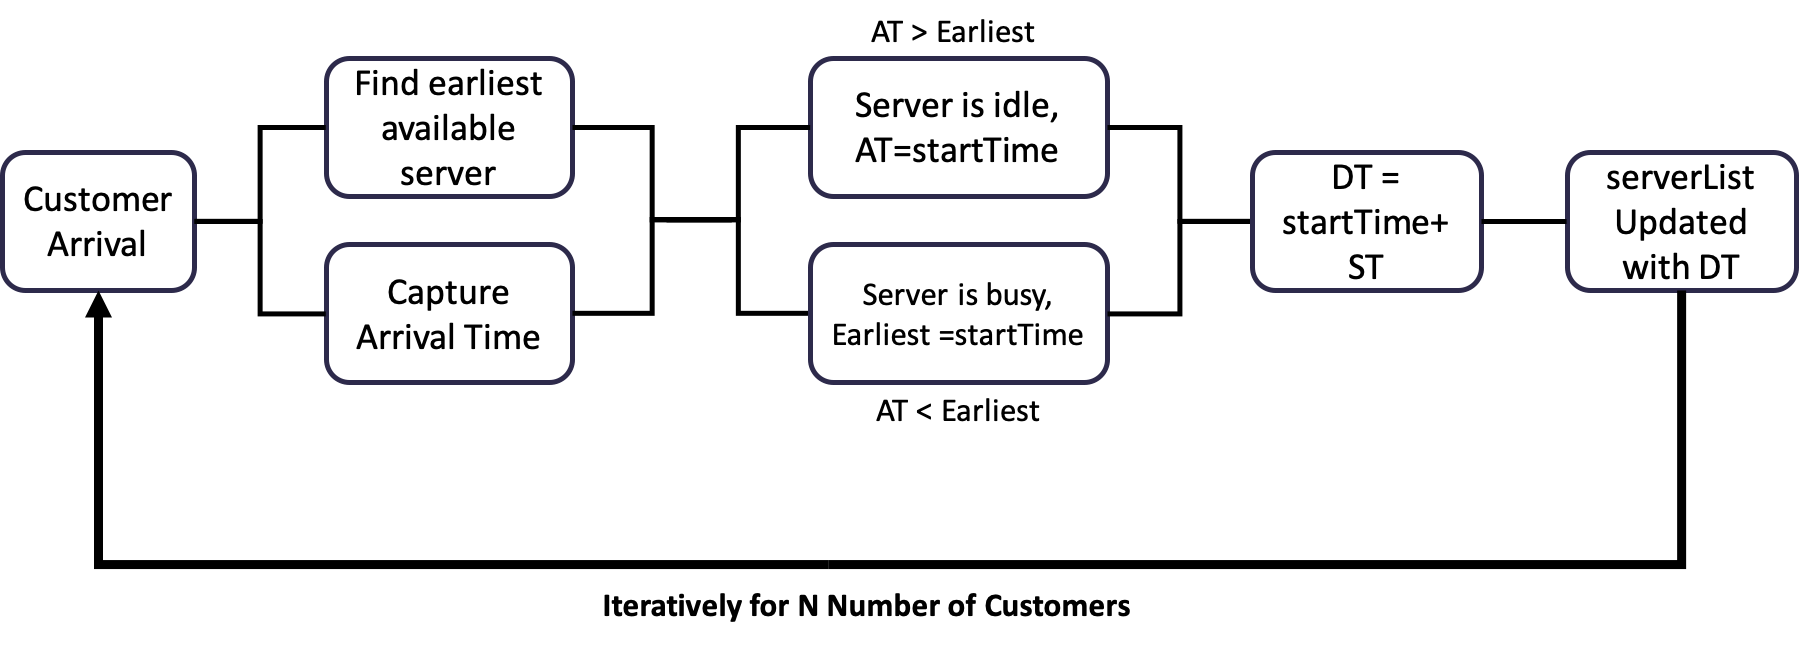
\includegraphics[width=400px]{images/main_simulation_loop.png}
  \caption{Main simulation loop diagram}
  \label{main_simualtion_loop_diagram}
\end{figure}

The MATLAB code for the main lines of the main simulation loop
are the following:
\begin{lstlisting}[style=Matlab-editor, basicstyle=\ttfamily\footnotesize]
%------simulation main loop-------
for i = 1:numCustomers
  % Find the earliest available server
  [~, idx] = min(serverList);
  earliestAvailableTime = serverList(idx);
  serverID(i) = idx;
  
  % Calculate the start time for the customer
  startTime = max(AT(i), earliestAvailableTime);
  startList(i) = startTime;
  
  % Calculate the departure time
  departureTime = startTime + ST(i);
  DT(i) = departureTime;
  
  % Update the server list
  serverList(idx) = departureTime;
  serviceTime(idx) = serviceTime(idx) + ST(i); 
end
\end{lstlisting}

\subsection{Track number of customers $N(t)$}
To compute the average number of customers and the PMF of $N(t)$,
we need to keep track of the number of customers at each time interval.
We determine the interval by using two variable; the first is 
\texttt{prevEventTime}, which stores the time of the last event and
the second is \texttt{clock}, which points to the current event.
The area under the curve of $N(t)$ is updated by adding the area 
after each arrival or departure event. The updated area is
\texttt{area = area + N * (clock - prevEventTime)}. The procedure for
computing the area under the curve of $N_q(t)$ is similar. To the PMF 
of $N(t)$, we need to compute the total time spent at each state $N$ and at the end of loop, 
the PMF is computed by dividing the total time spent in state $N$ by the total 
simulation time, which is the last departure time or \texttt{clock}. 

{\color{red} \textbf{Note:} The departure times must be sorted from smallest to largest
before starting the tracking process}

\begin{figure}[H]
  \vspace{2em}
  \centering 
  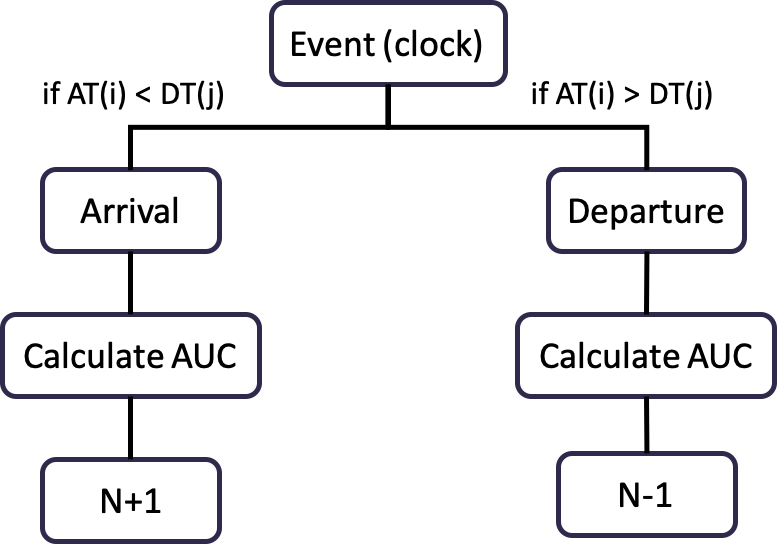
\includegraphics[width=250px]{images/track_N.png}
  \caption{The process of tracking the number of customers and computing $E[N]$}
\end{figure}

The MATLAB code for the main lines of tracking $N(t)$ are the following 
\begin{lstlisting}[style=Matlab-editor, basicstyle=\ttfamily\footnotesize]
  function [areaN, areaNq, simPMF] = PMF_and_track_N(AT, DT, c, N_max)
    N = 0; simPMF = zeros(1, N_max+1);
    areaN = 0; areaNq = 0;
    preEventTime = 0; clock = 0;
    i = 1; j = 1;
    sortedDT = sort(DT);
    while clock < max(AT)
        if AT(i) < sortedDT(j)
            clock = AT(i);
            timeInterval = clock - preEventTime;
            simPMF(min(N, N_max)+1) = simPMF(min(N, N_max)+1) + timeInterval;
            areaN = areaN + timeInterval * N;
            areaNq = areaNq + timeInterval * max(0, N - c);
            N = N + 1;
            preEventTime = clock;
            i = i + 1;
        else
            clock = sortedDT(j);
            timeInterval = clock - preEventTime;
            simPMF(min(N, N_max)+1) = simPMF(min(N, N_max)+1) + timeInterval;
            areaN = areaN + timeInterval * N;
            areaNq = areaNq + timeInterval * max(0, N - c);
            N = N - 1;
            preEventTime = clock;
            j = j + 1;
        end
    end

    for j = j:1:length(sortedDT)
        clock = sortedDT(j);
        timeInterval = clock - preEventTime;
        simPMF(min(N, N_max)+1) = simPMF(min(N, N_max)+1) + timeInterval;
        areaN = areaN + timeInterval * N;
        areaNq = areaNq + timeInterval * max(0, N - c);
        N = N - 1;
        preEventTime = clock;
    end 
    simPMF = simPMF/clock;
end
\end{lstlisting}




\newpage
\section{Results and Discussion}
\subsection{$E[T], E[W], E[N]$, and  $E[N_q]$}
\begin{figure}[H]
  \centering
  \subfloat[]{
    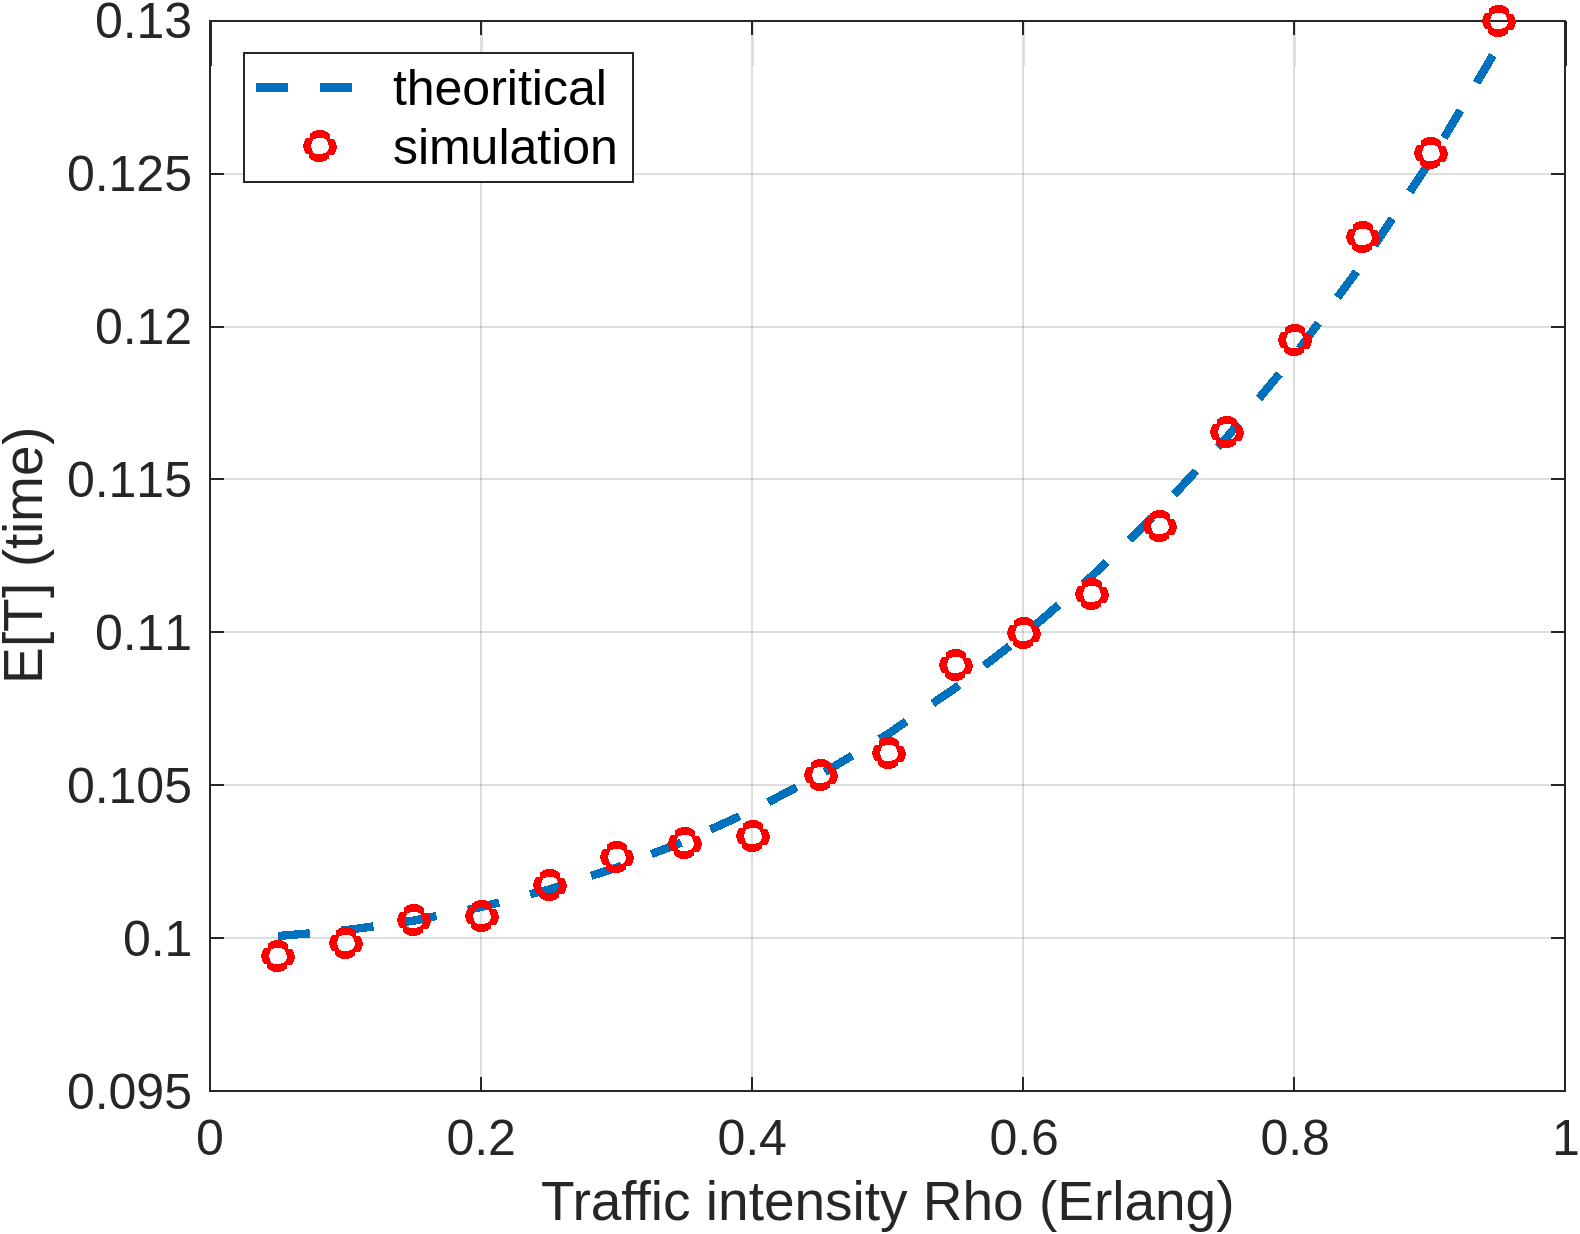
\includegraphics[width=200px]{../code/figures/avgs_vs_traffic_intensity/E_T.png}
  }  
  \subfloat[]{
    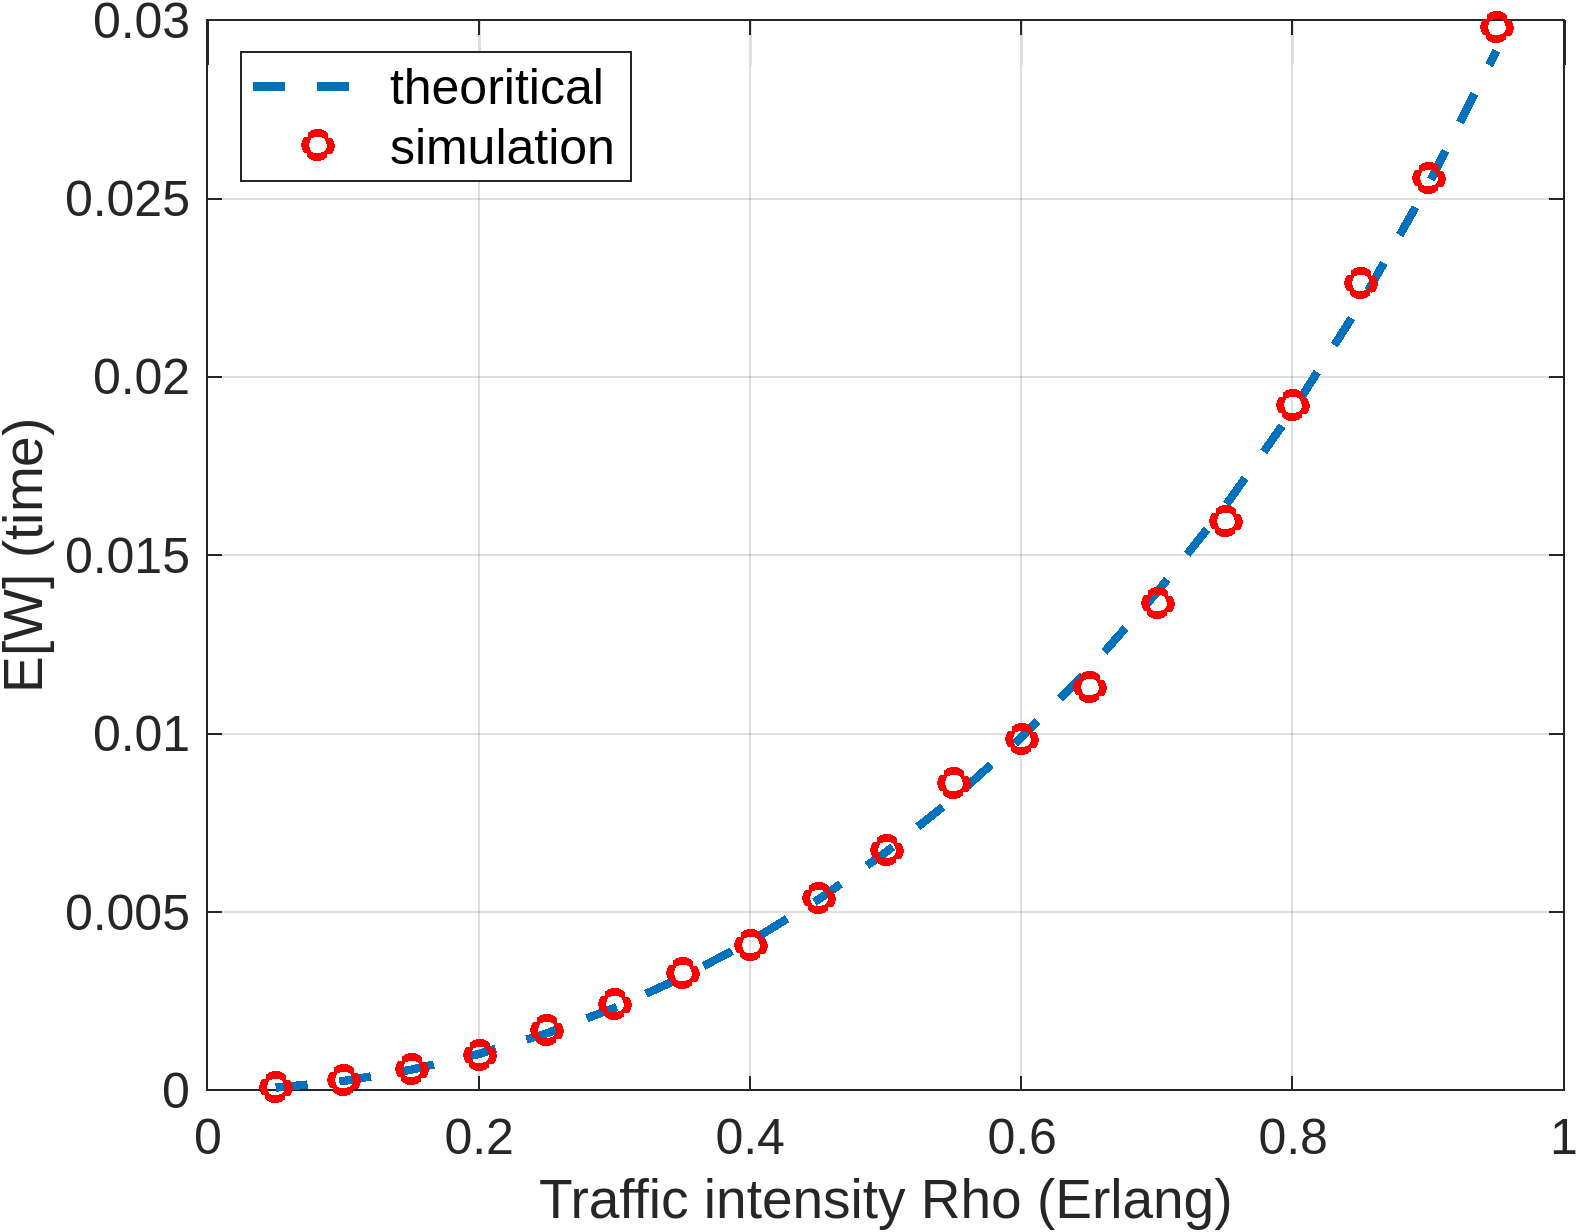
\includegraphics[width=200px]{../code/figures/avgs_vs_traffic_intensity/E_W.png}
  } 
  \hspace{0px}
  \subfloat[]{
    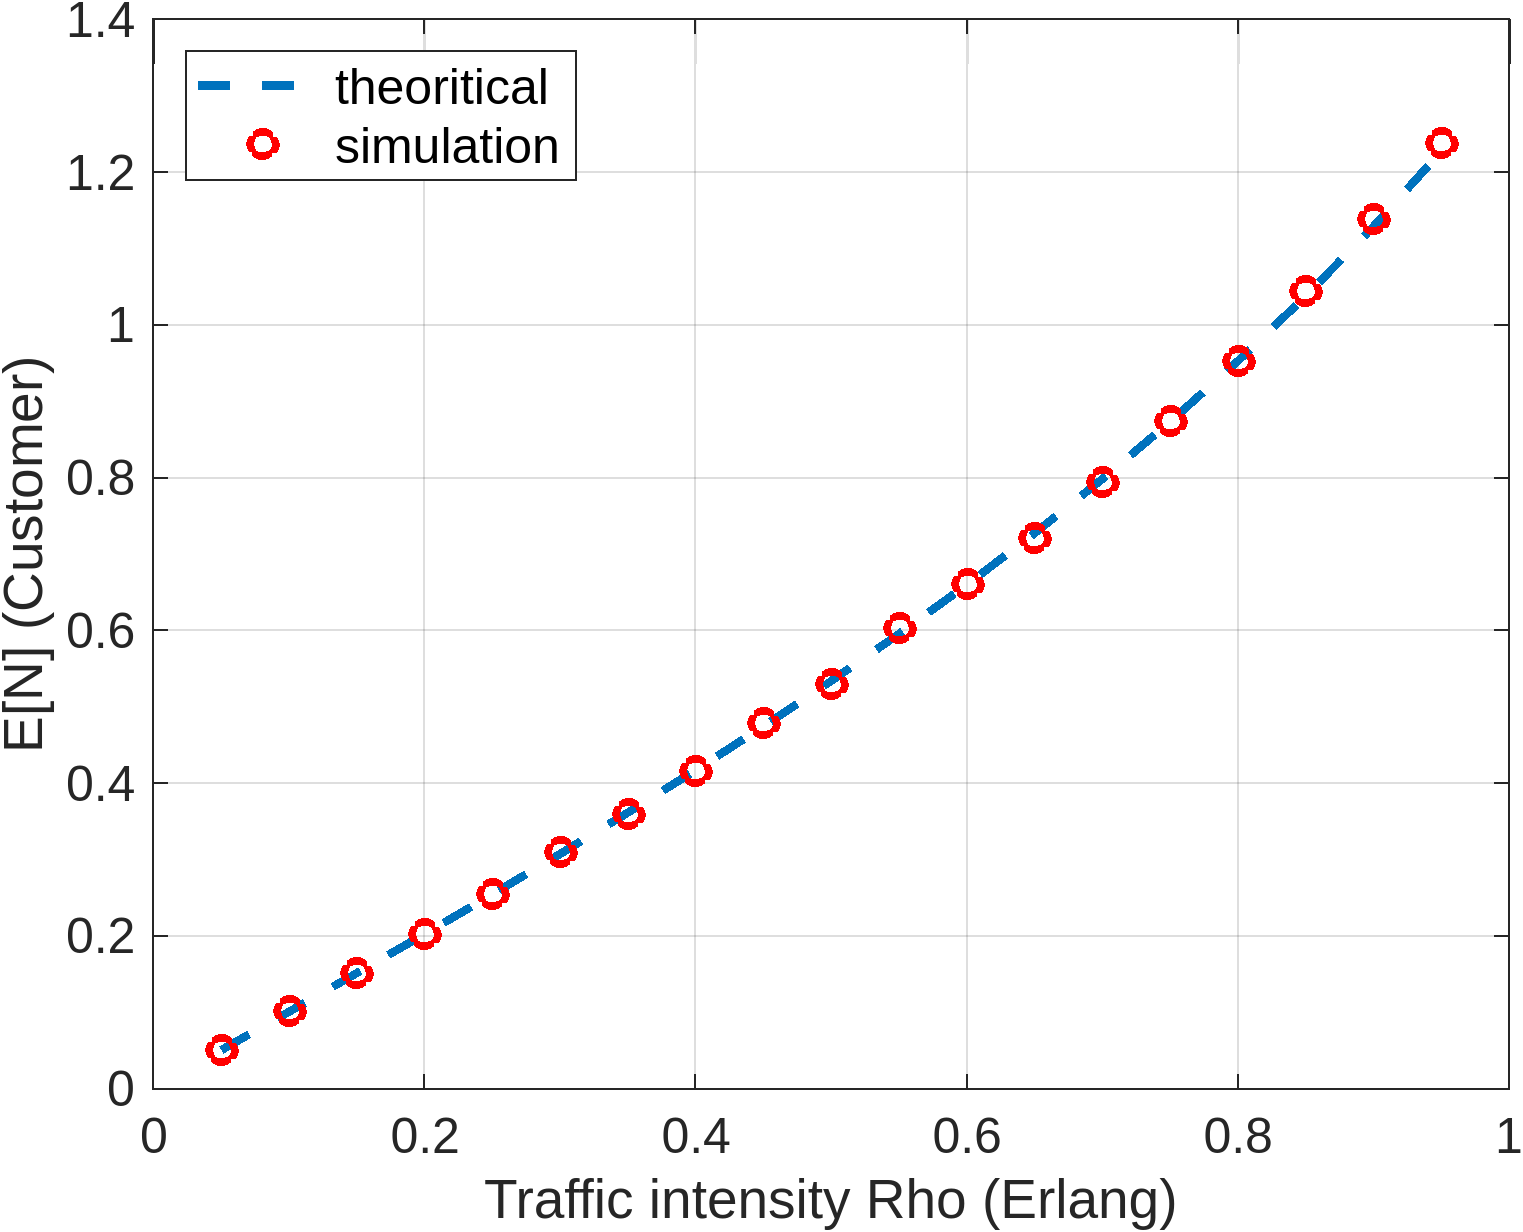
\includegraphics[width=200px]{../code/figures/avgs_vs_traffic_intensity/E_N.png}
  } 
  \subfloat[]{
    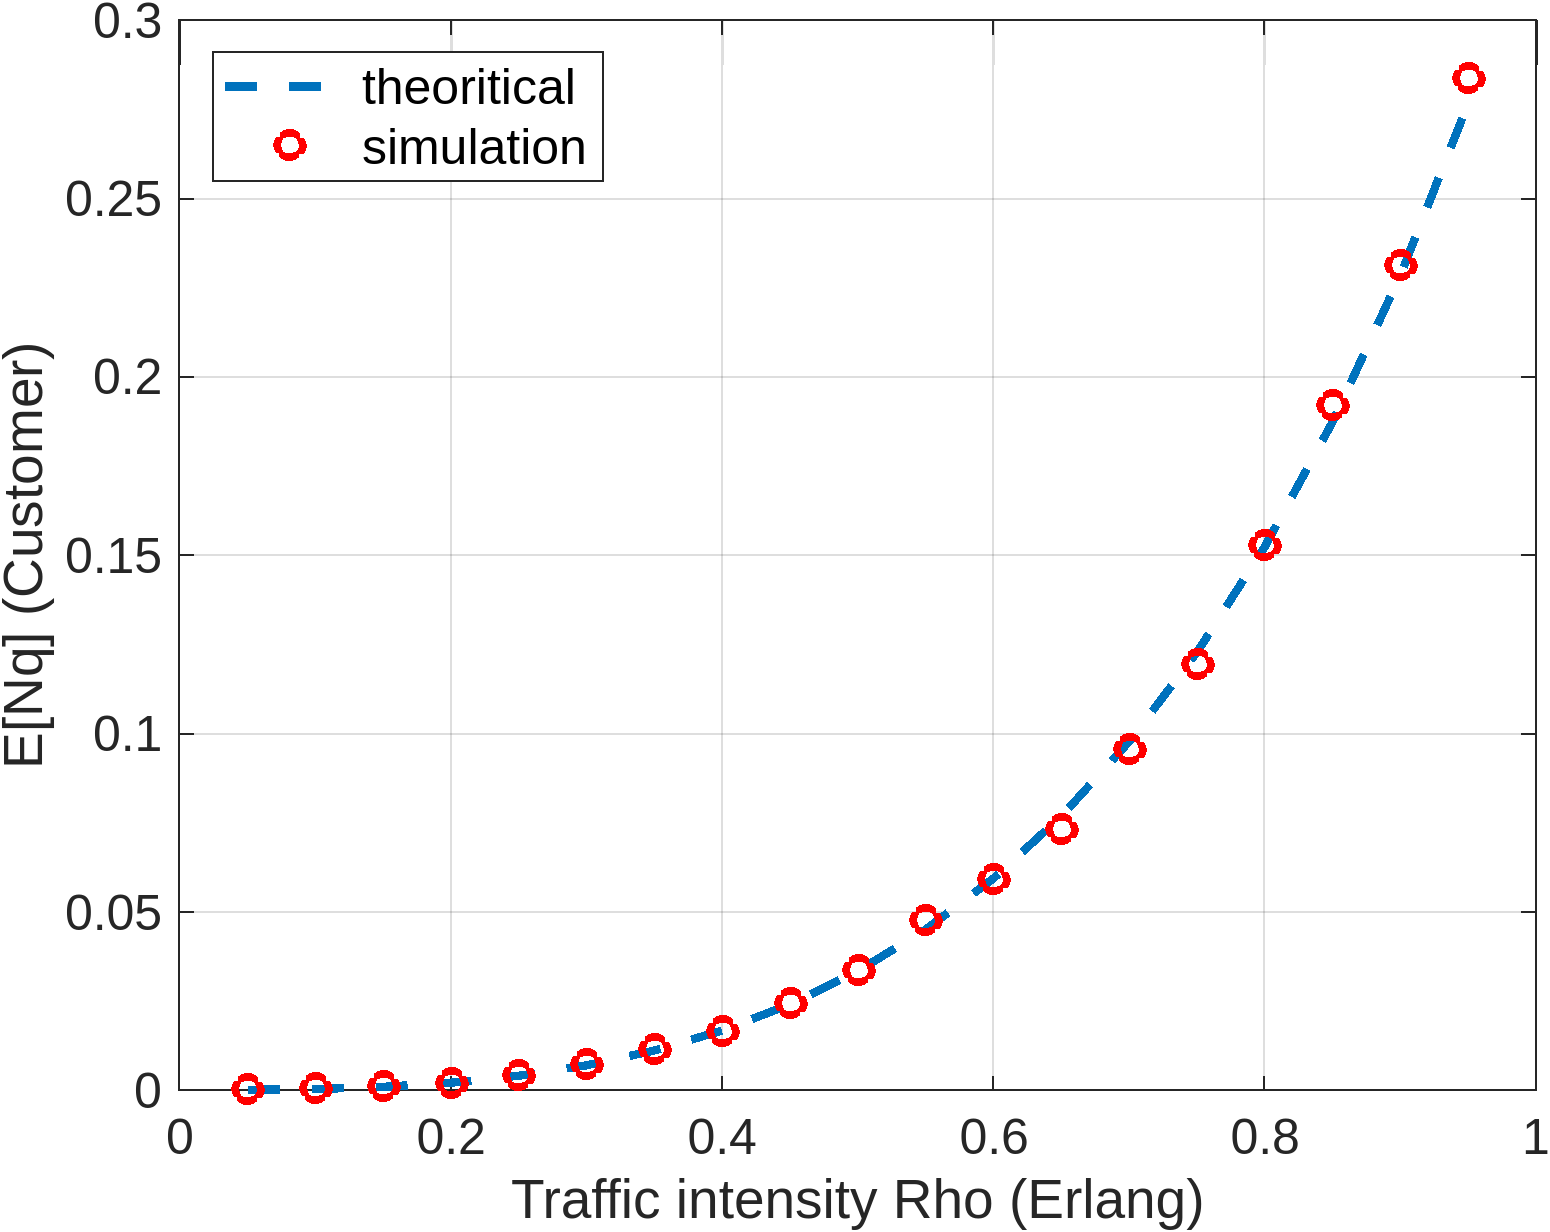
\includegraphics[width=200px]{../code/figures/avgs_vs_traffic_intensity/E_Nq.png}
  } 
  \caption{$E[T], E[W], E[N], \text{and}, E[N_q]$ 
  \\ as function of the traffic intensity (for $c=2$)}
  \label{avg_vs_rho}
\end{figure}

Figure \ref{avg_vs_rho} shows plots for the average total time spent 
in the system $E[T]$, the average waiting time in  the buffer $E[W]$,
the average number of customers in the system $E[N]$, and the average 
number of customers in the buffer $E[N_q]$. All quantities increase as
the traffic intensity increases, which is expected since the increase 
of the traffic intensity implies that the arrival rate to the system is 
getting relatively close to the overall service rate of the system. This means 
that the system is becoming more saturated and hence the averages for 
the total time, the waiting time, and the total number of customers
in the system and in the buffer increase. Furthermore, Figure \ref{avg_vs_rho} 
shows that the simulation results agree with the theoretical ones.

\subsection{PDF of the total time}
\begin{figure}[H]
  \centering
  \subfloat[]{
    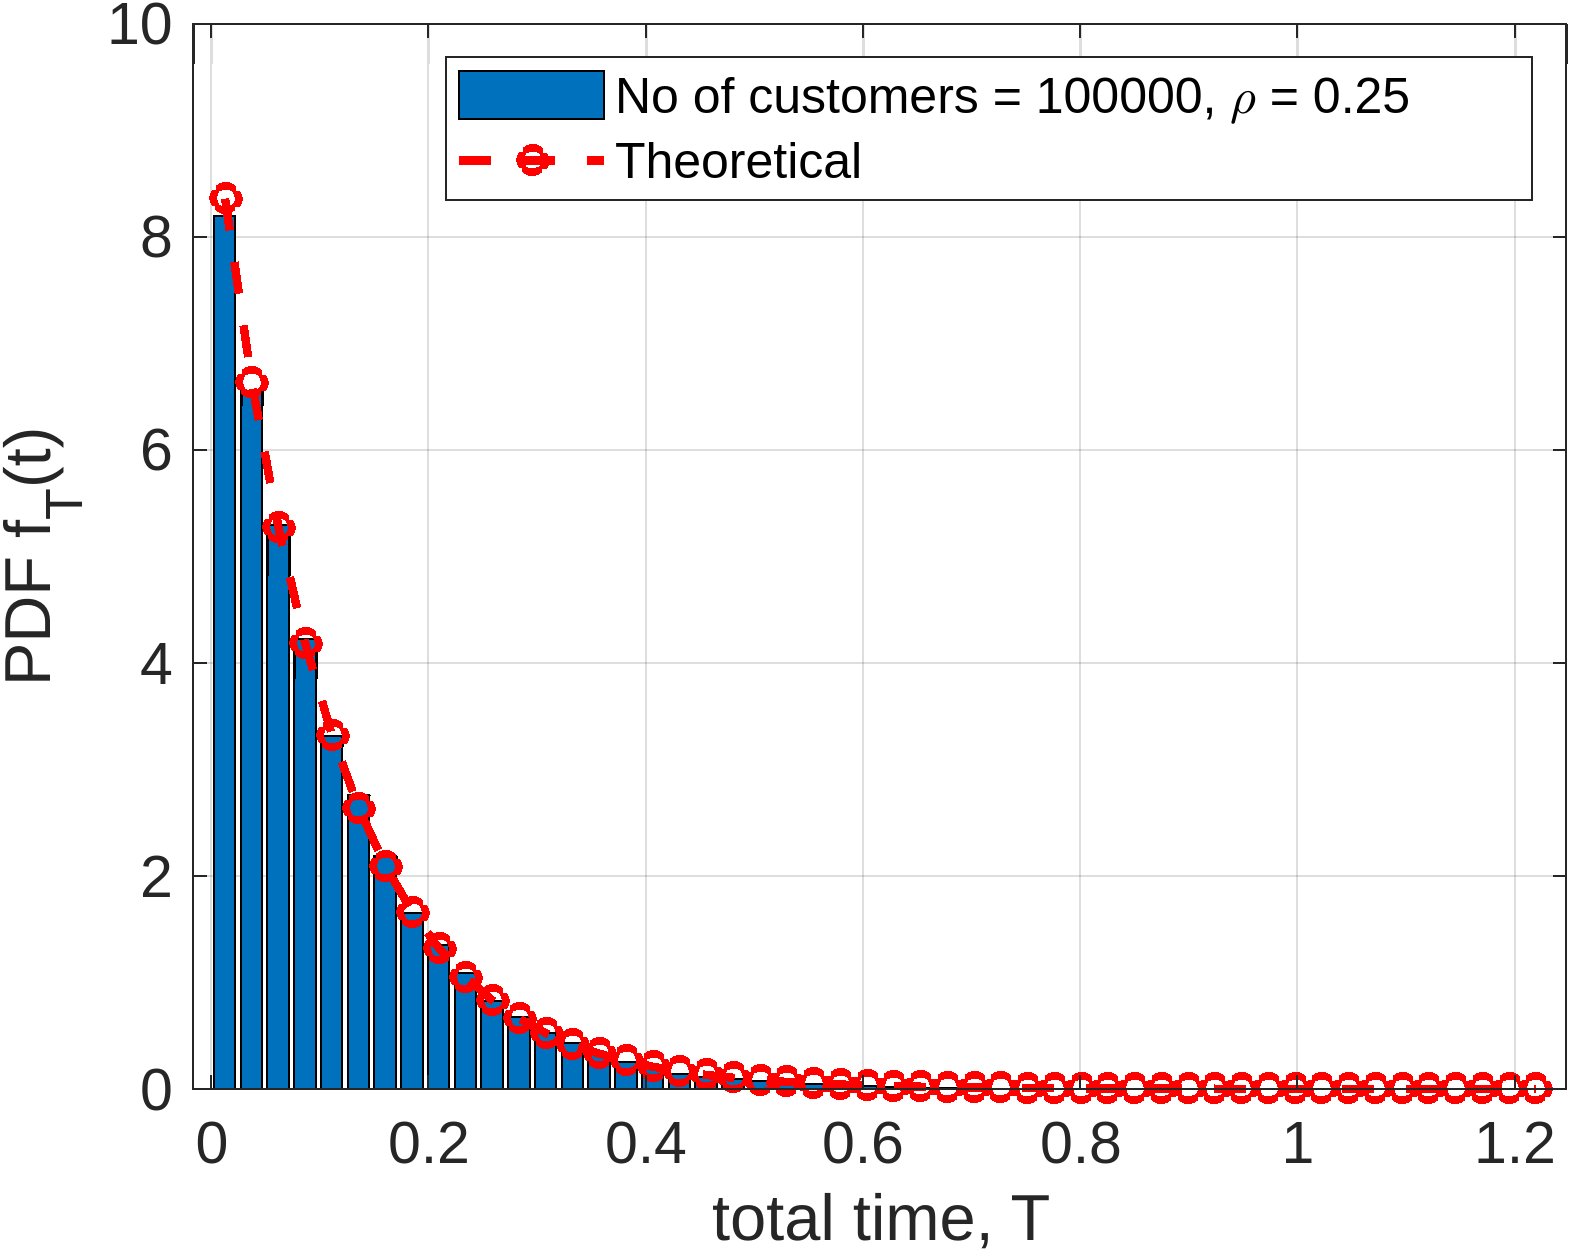
\includegraphics[width=200px]{../code/figures/total_time_dist/bars_plot_no_customers_100000_rho_0.25.png}
  }
  \subfloat[]{
    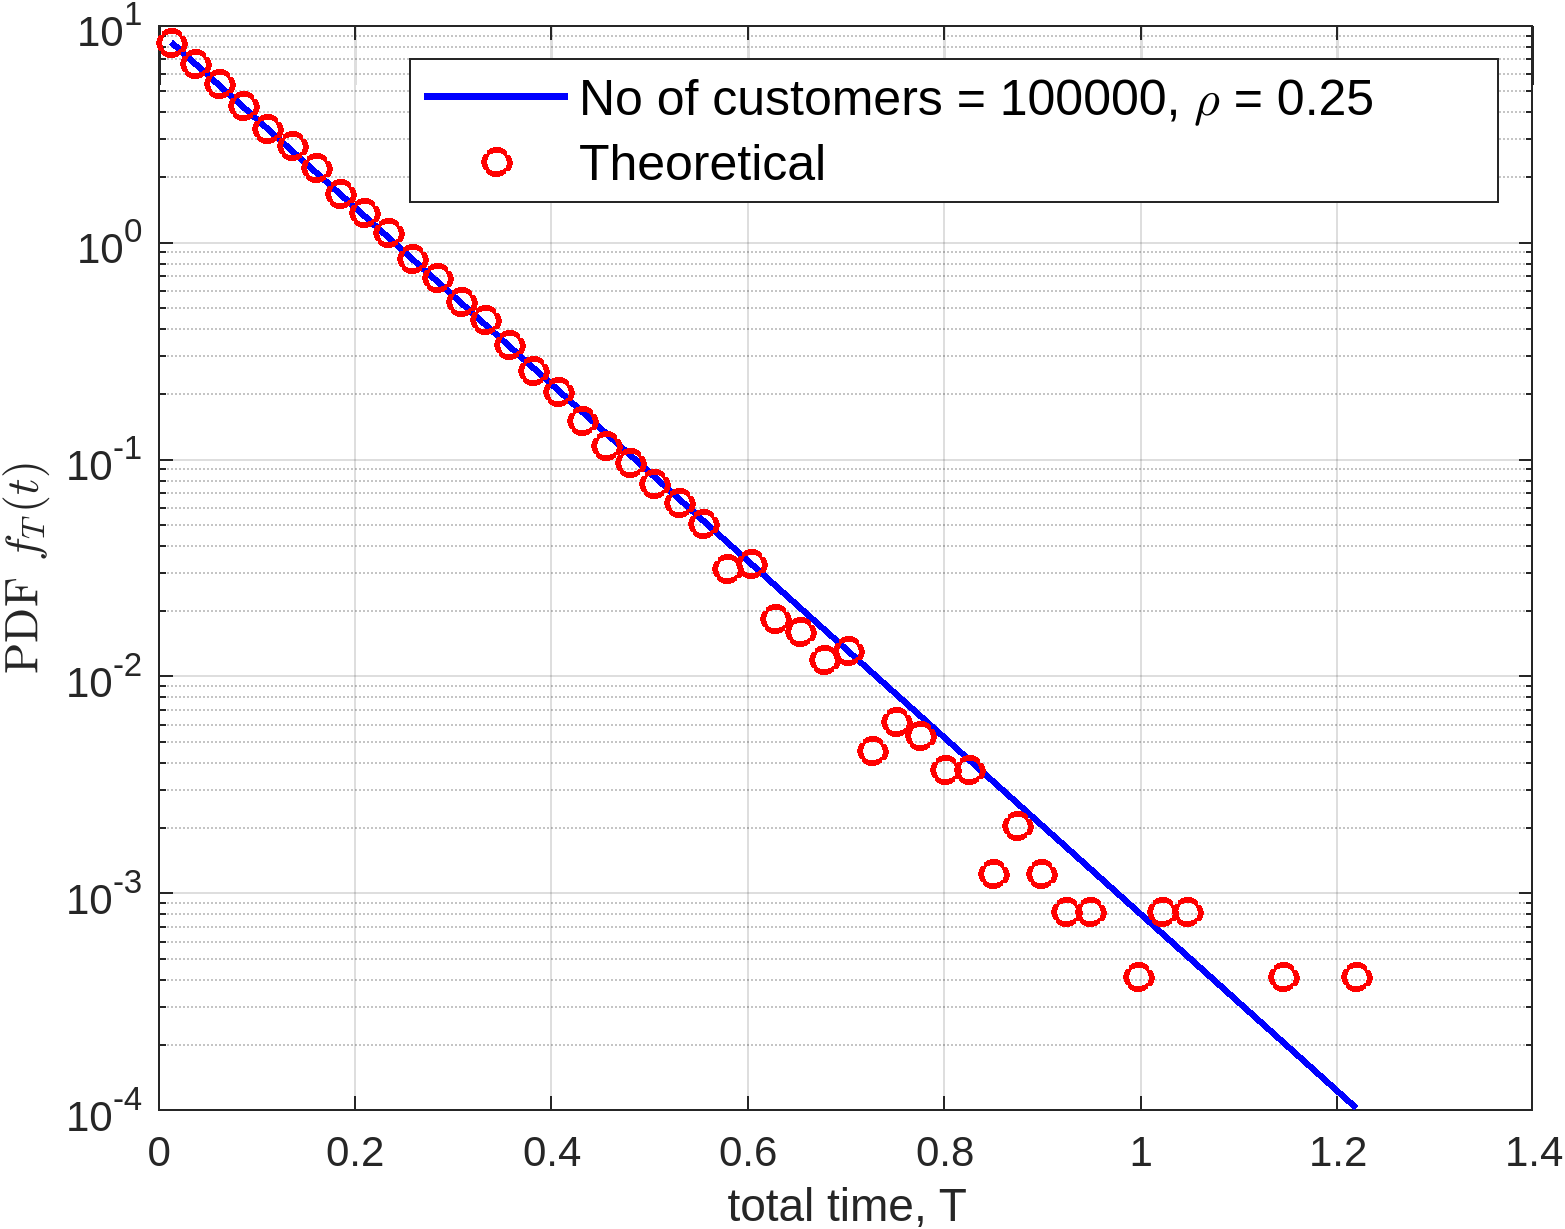
\includegraphics[width=200px]{../code/figures/total_time_dist/semilogy_plot_no_customers_100000_rho_0.25.png}
  }
  \hspace{0px}
  \subfloat[]{
    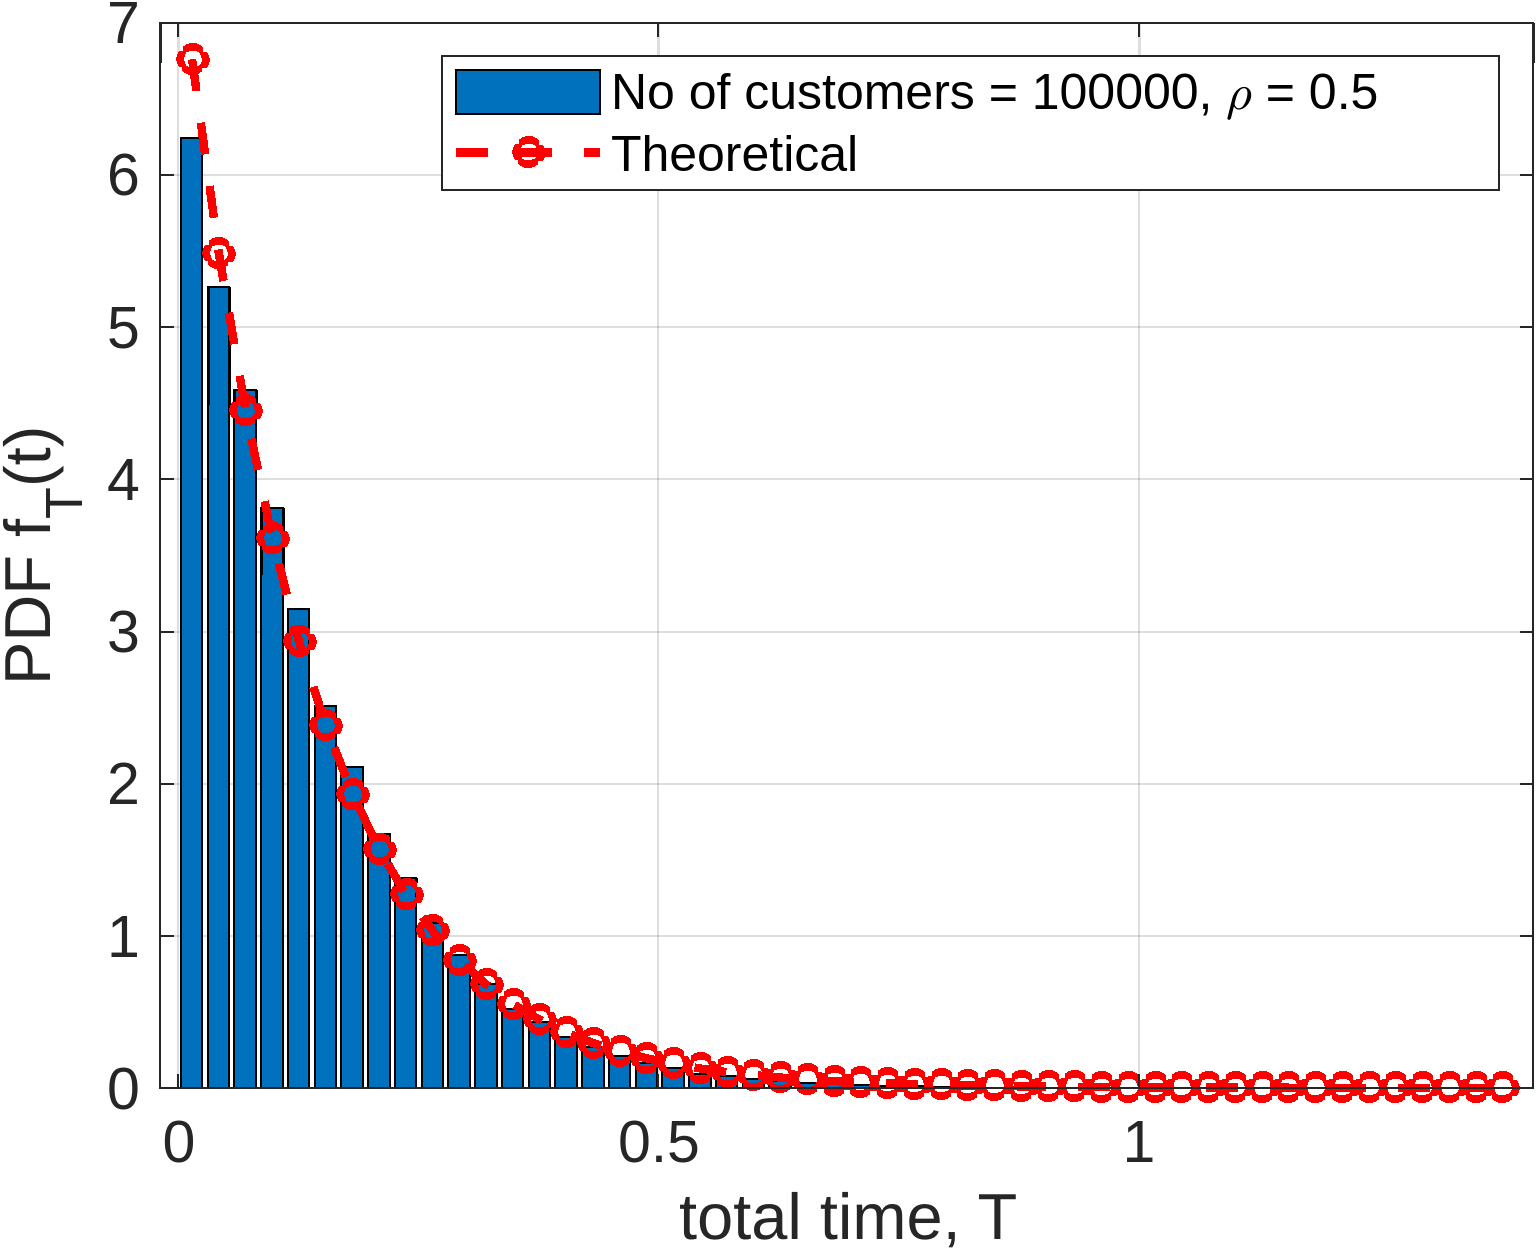
\includegraphics[width=200px]{../code/figures/total_time_dist/bars_plot_no_customers_100000_rho_0.5.png}
  }
  \subfloat[]{
    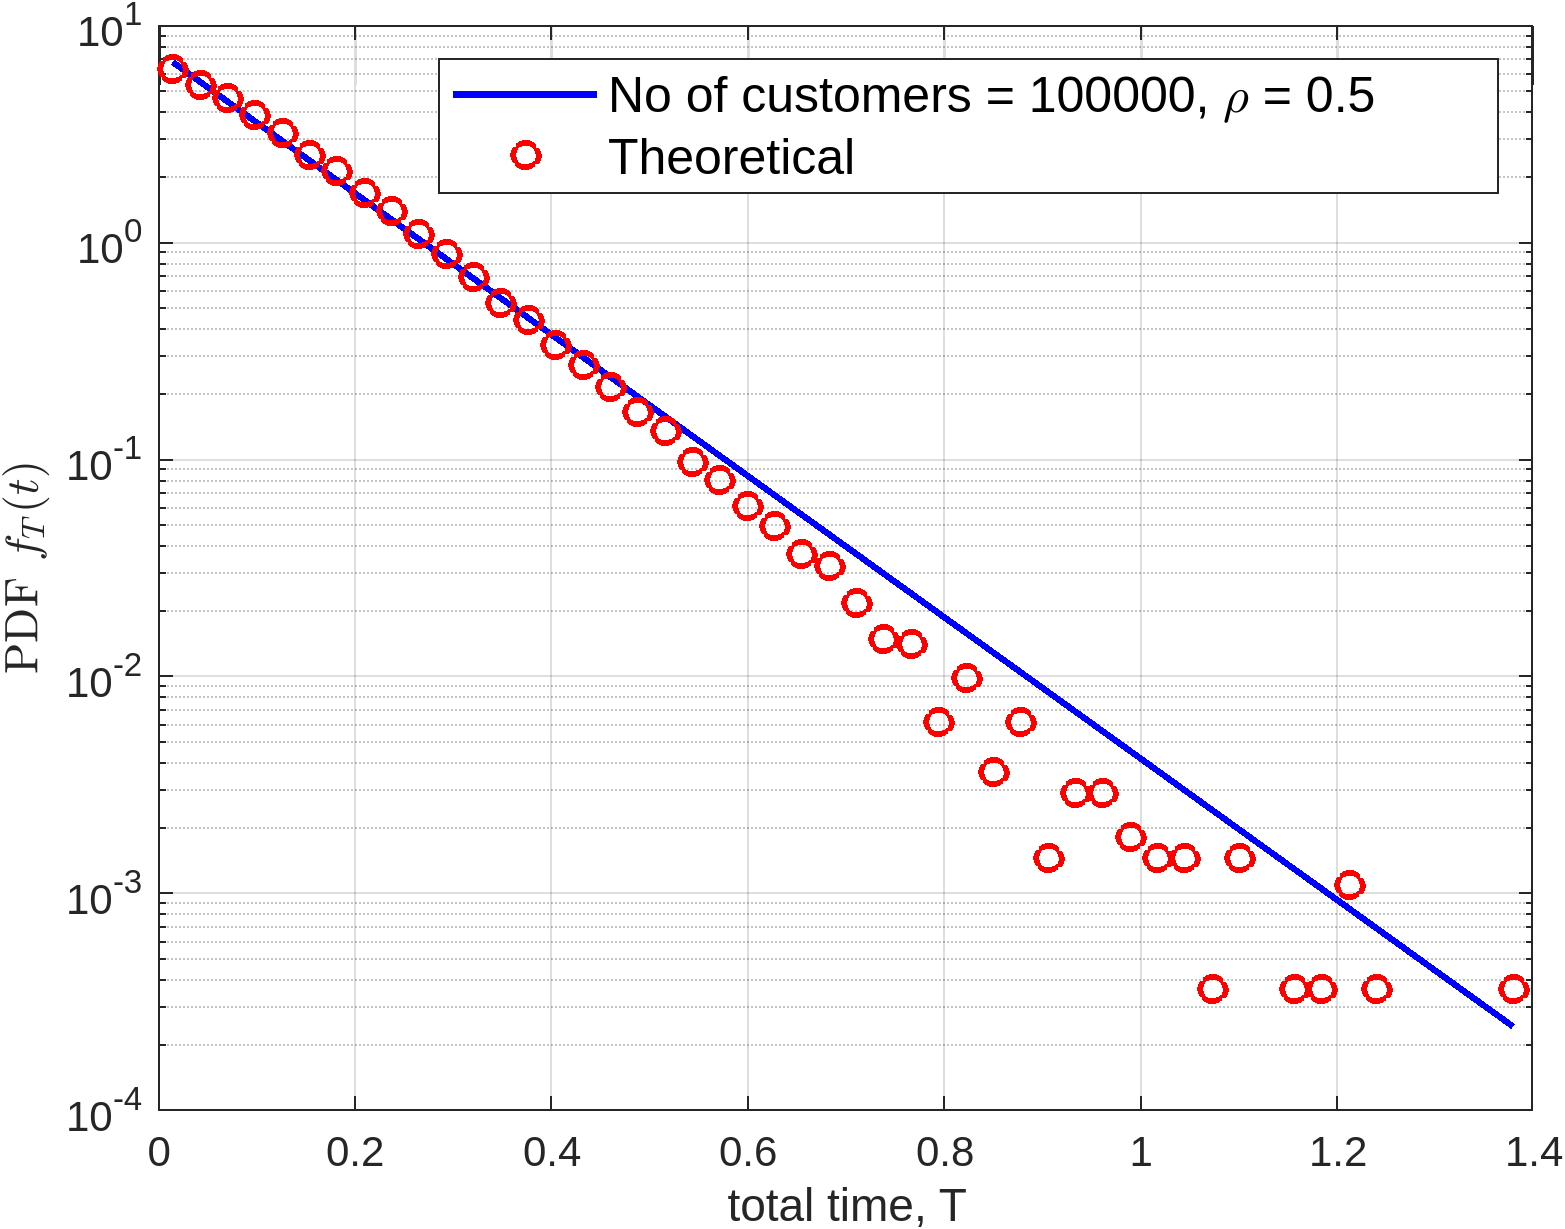
\includegraphics[width=200px]{../code/figures/total_time_dist/semilogy_plot_no_customers_100000_rho_0.5.png}
  }
  \caption{PDF of the total time in the system for low and medium traffic intensity}
  \label{PDF_TT_low_med}
\end{figure}

\begin{figure}[H]
  \centering
  \subfloat[]{
    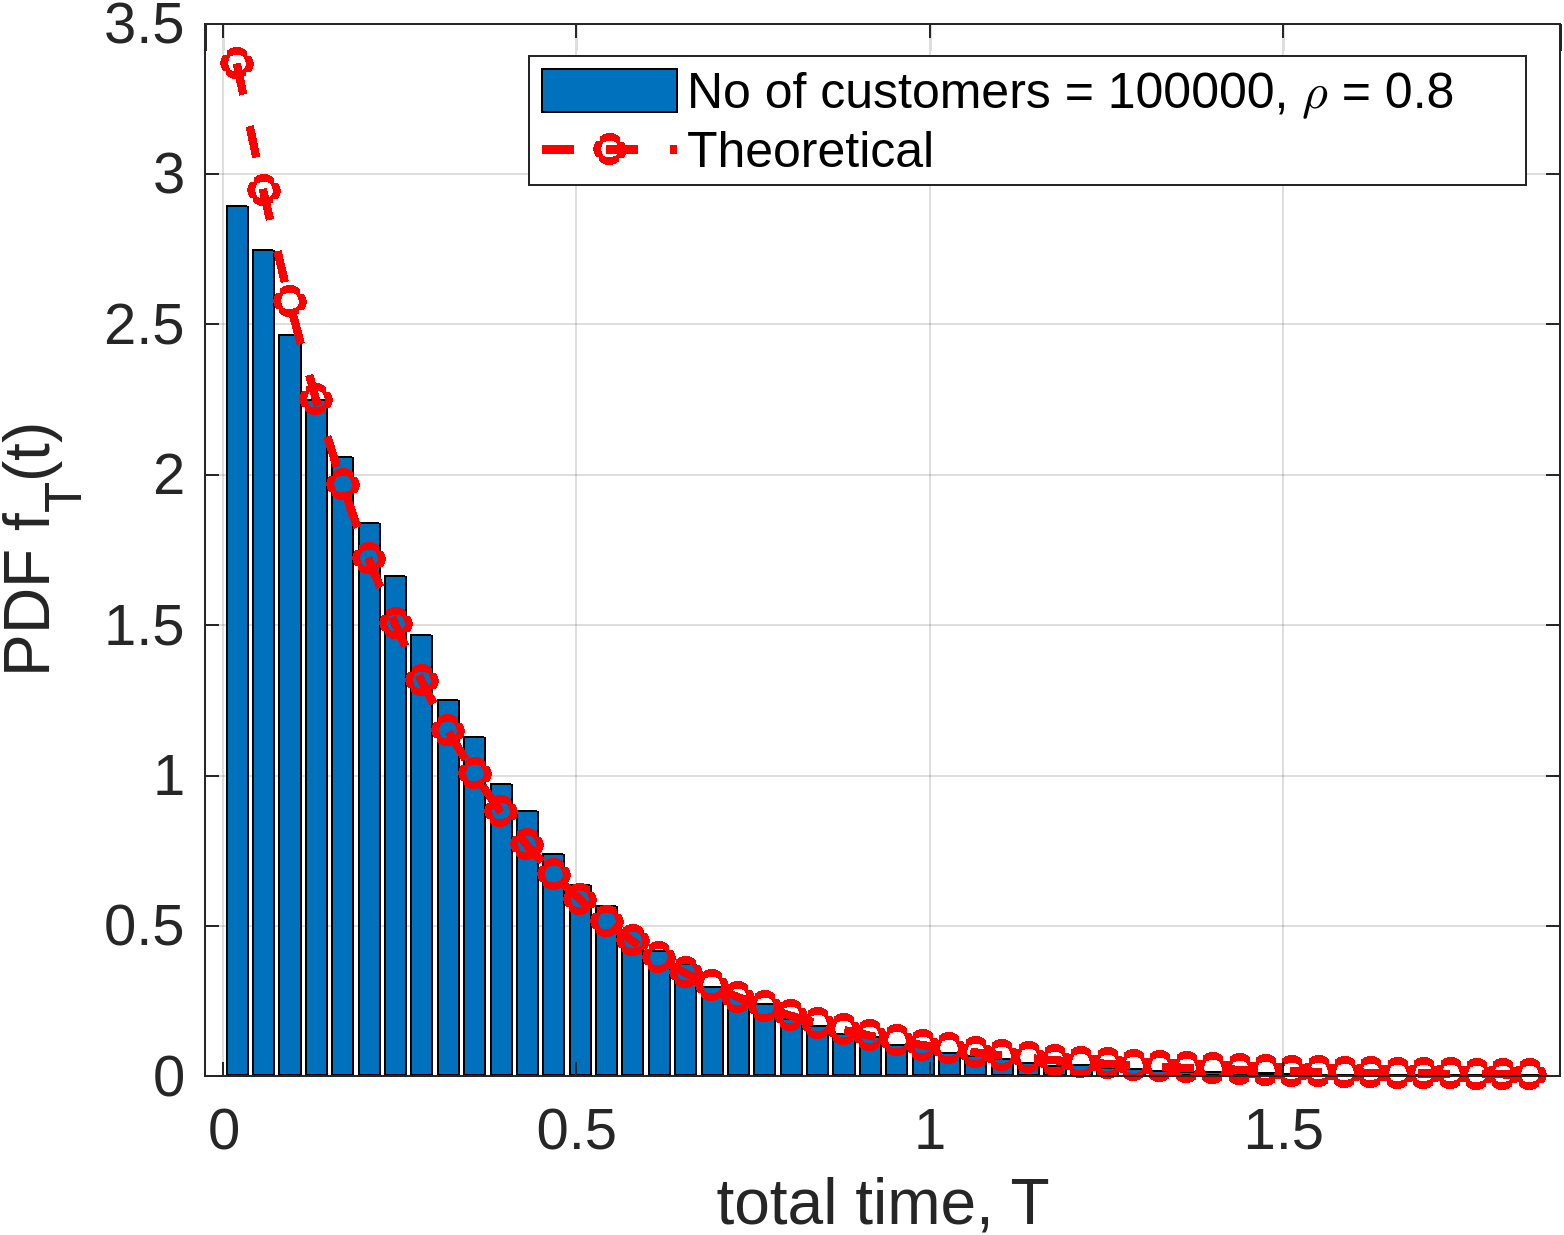
\includegraphics[width=200px]{../code/figures/total_time_dist/bars_plot_no_customers_100000_rho_0.8.png}
  }
  \subfloat[]{
    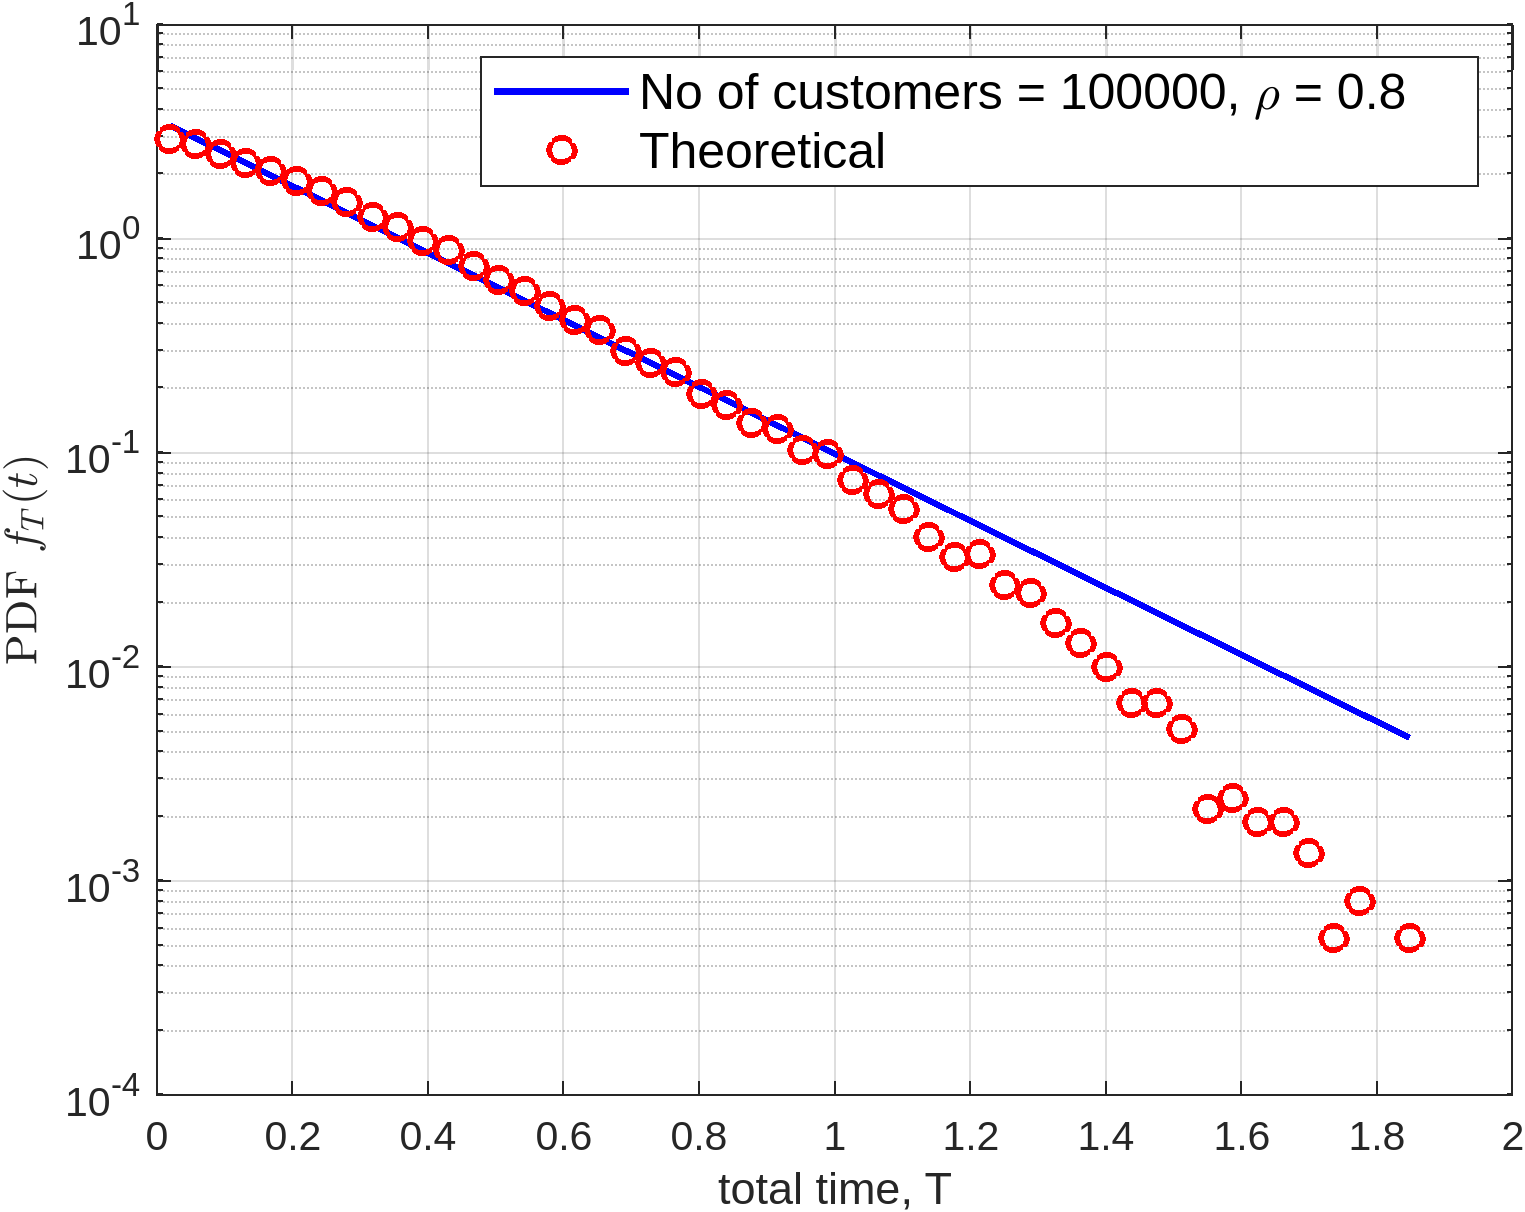
\includegraphics[width=200px]{../code/figures/total_time_dist/semilogy_plot_no_customers_100000_rho_0.8.png}
  }
  \hspace{0px}
  \subfloat[]{
    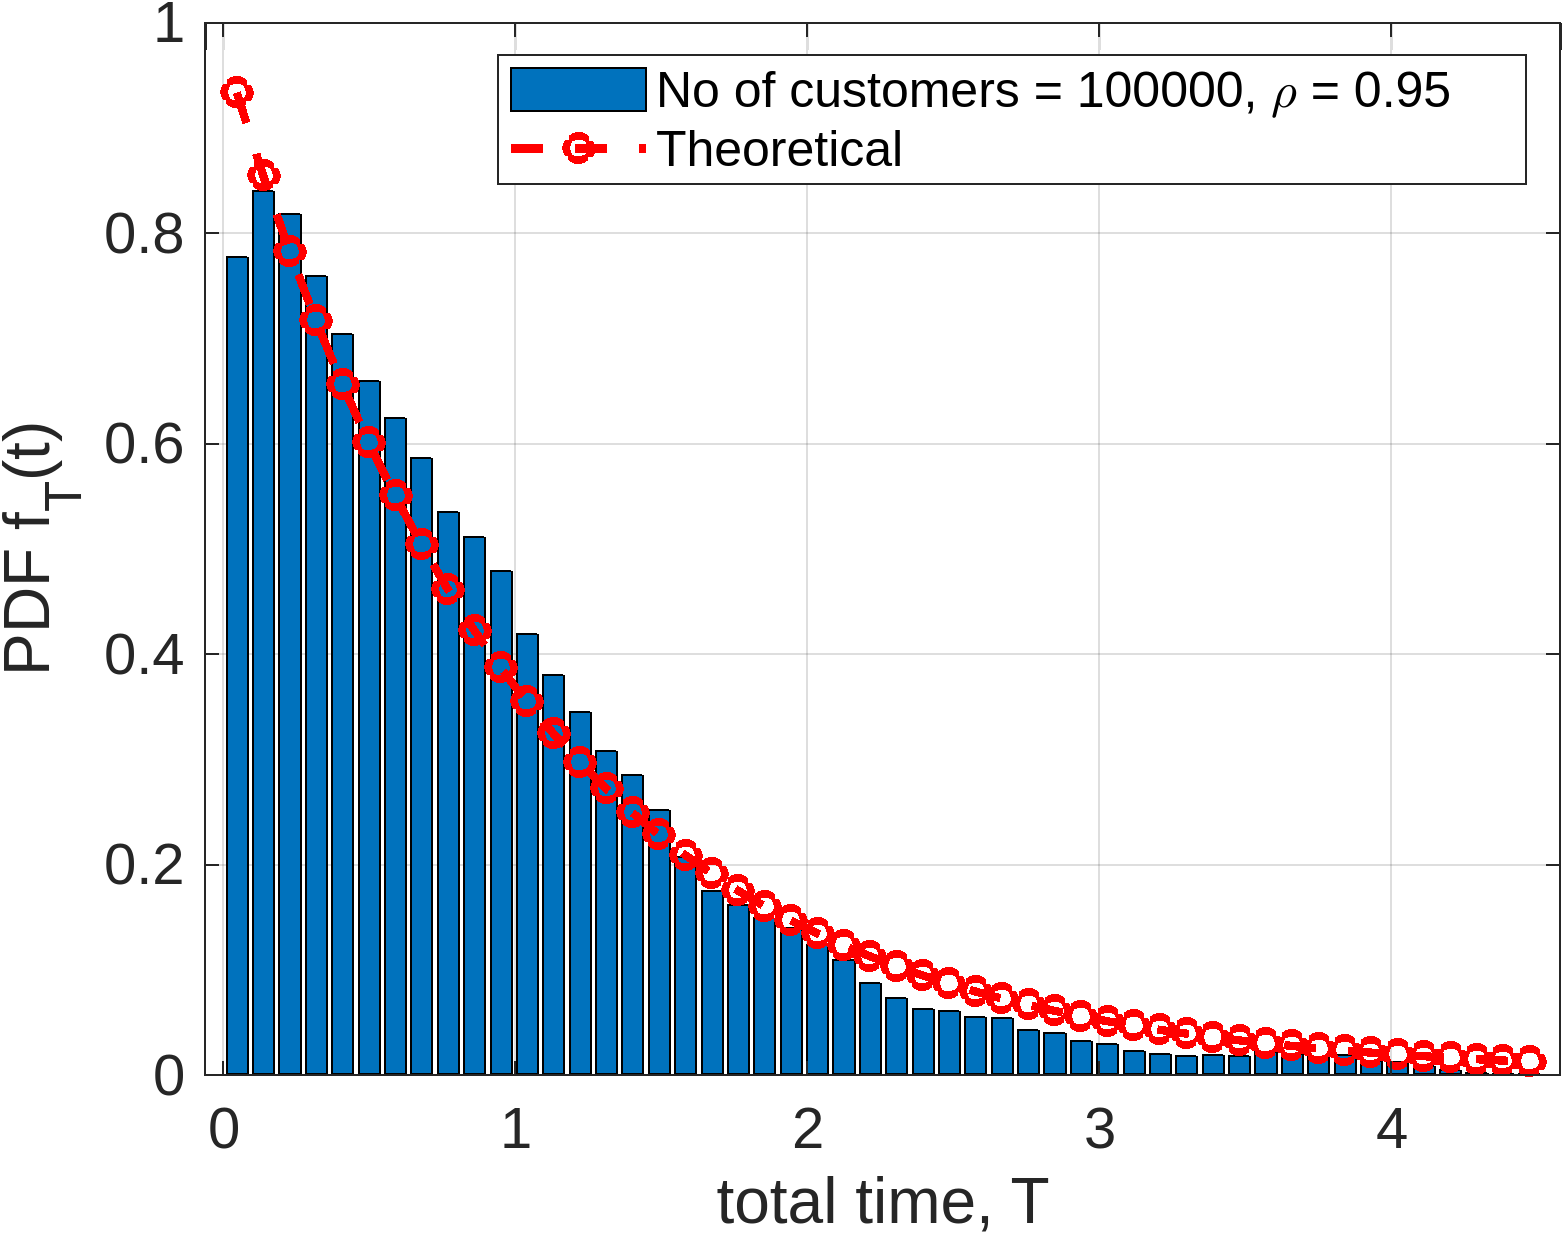
\includegraphics[width=200px]{../code/figures/total_time_dist/bars_plot_no_customers_100000_rho_0.95.png}
  }
  \subfloat[]{
    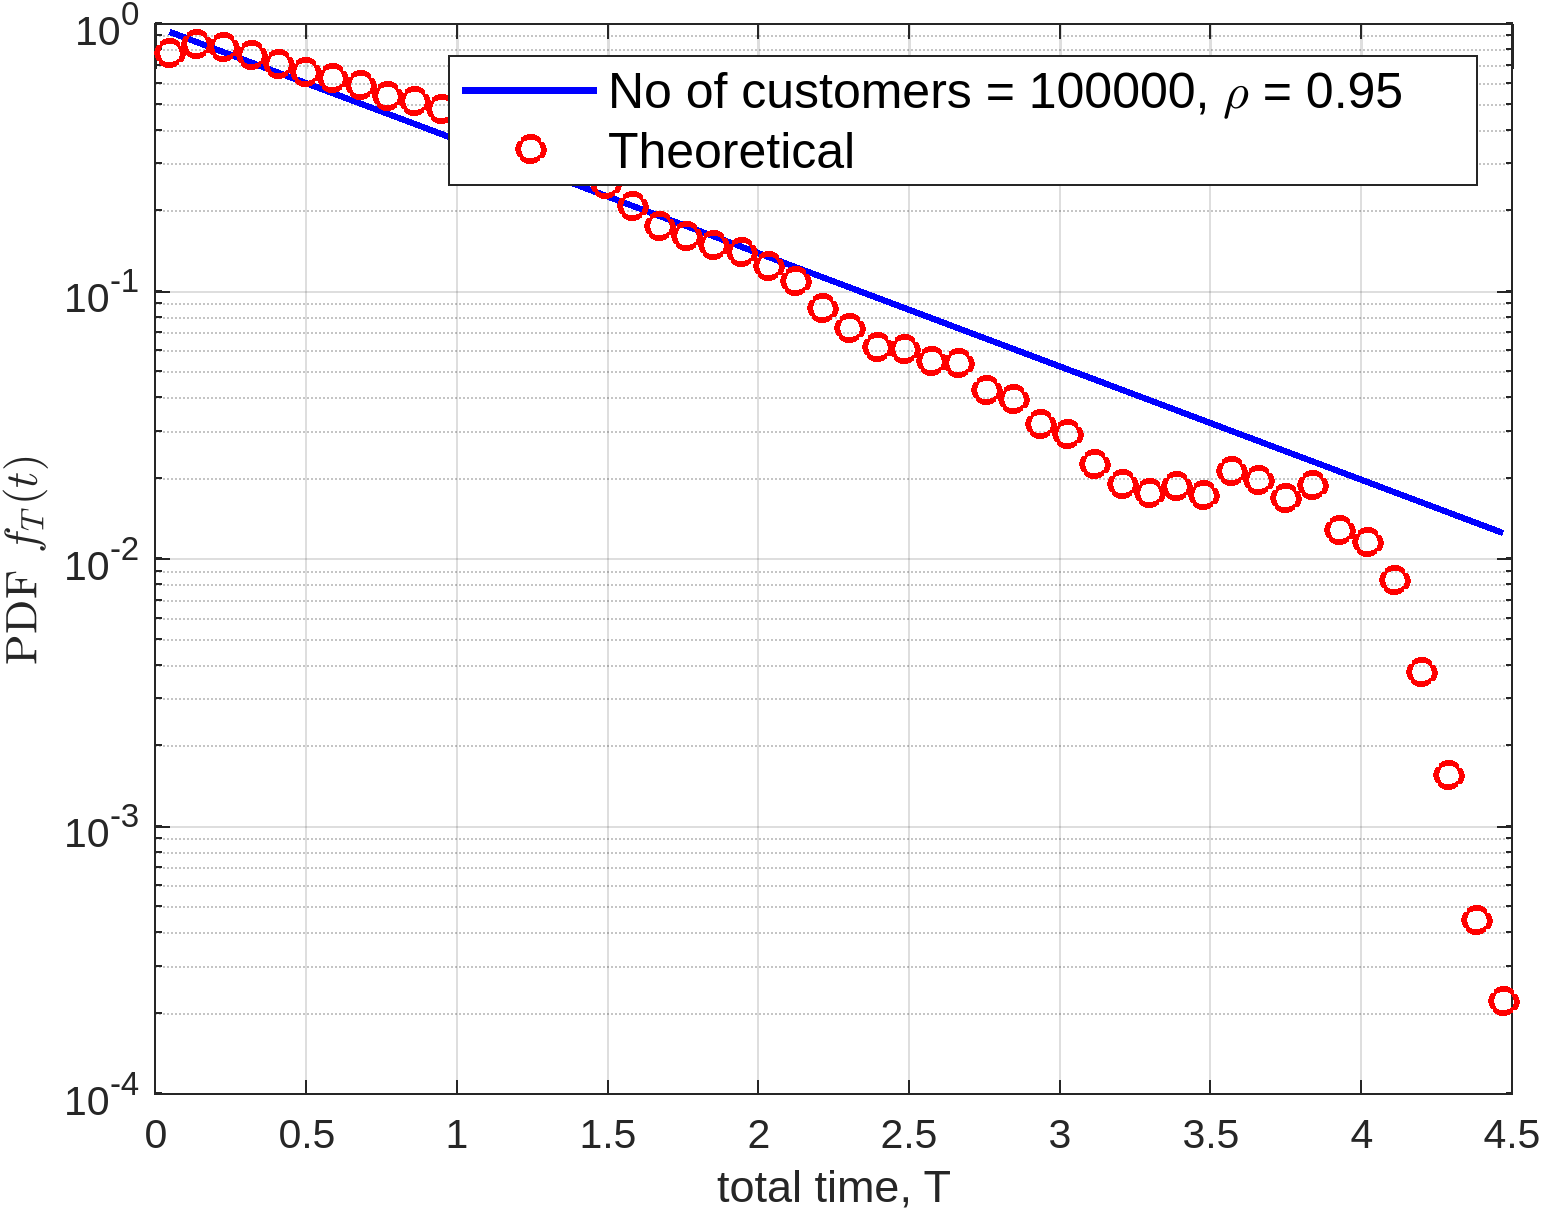
\includegraphics[width=200px]{../code/figures/total_time_dist/semilogy_plot_no_customers_100000_rho_0.95.png}
  }
  \caption{PDF of the total time in the system for high traffic intensity}
  \label{PDF_TT_high}
\end{figure}

Figure \ref{PDF_TT_low_med} shows the probability density function (PDF) 
for the total time spent in the system for a low traffic intensity, $\rho = 0.25$
and a medium traffic intensity, $\rho=0.5$. The distribution is exponential as expected
from the theoretical formula. Moreover, the empirical and the theoretical distributions
are in an excellent agreement.

Figure \ref{PDF_TT_high} shows the PDF for the total time for high traffic intensities, 
$\rho=0.8$ and $\rho=0.95$. They agree with the theoretical ones, but not as well as 
in the case of low and medium traffic intensities. In an attempt to resolve this issue,
we increased the number of customers to $1000000$ as indicated in Figure \ref{PDF_TT_high_more_cus}.
This resulted in a better agreement with the theoretical results.

\begin{figure}[H]
  \centering
  \subfloat[]{
    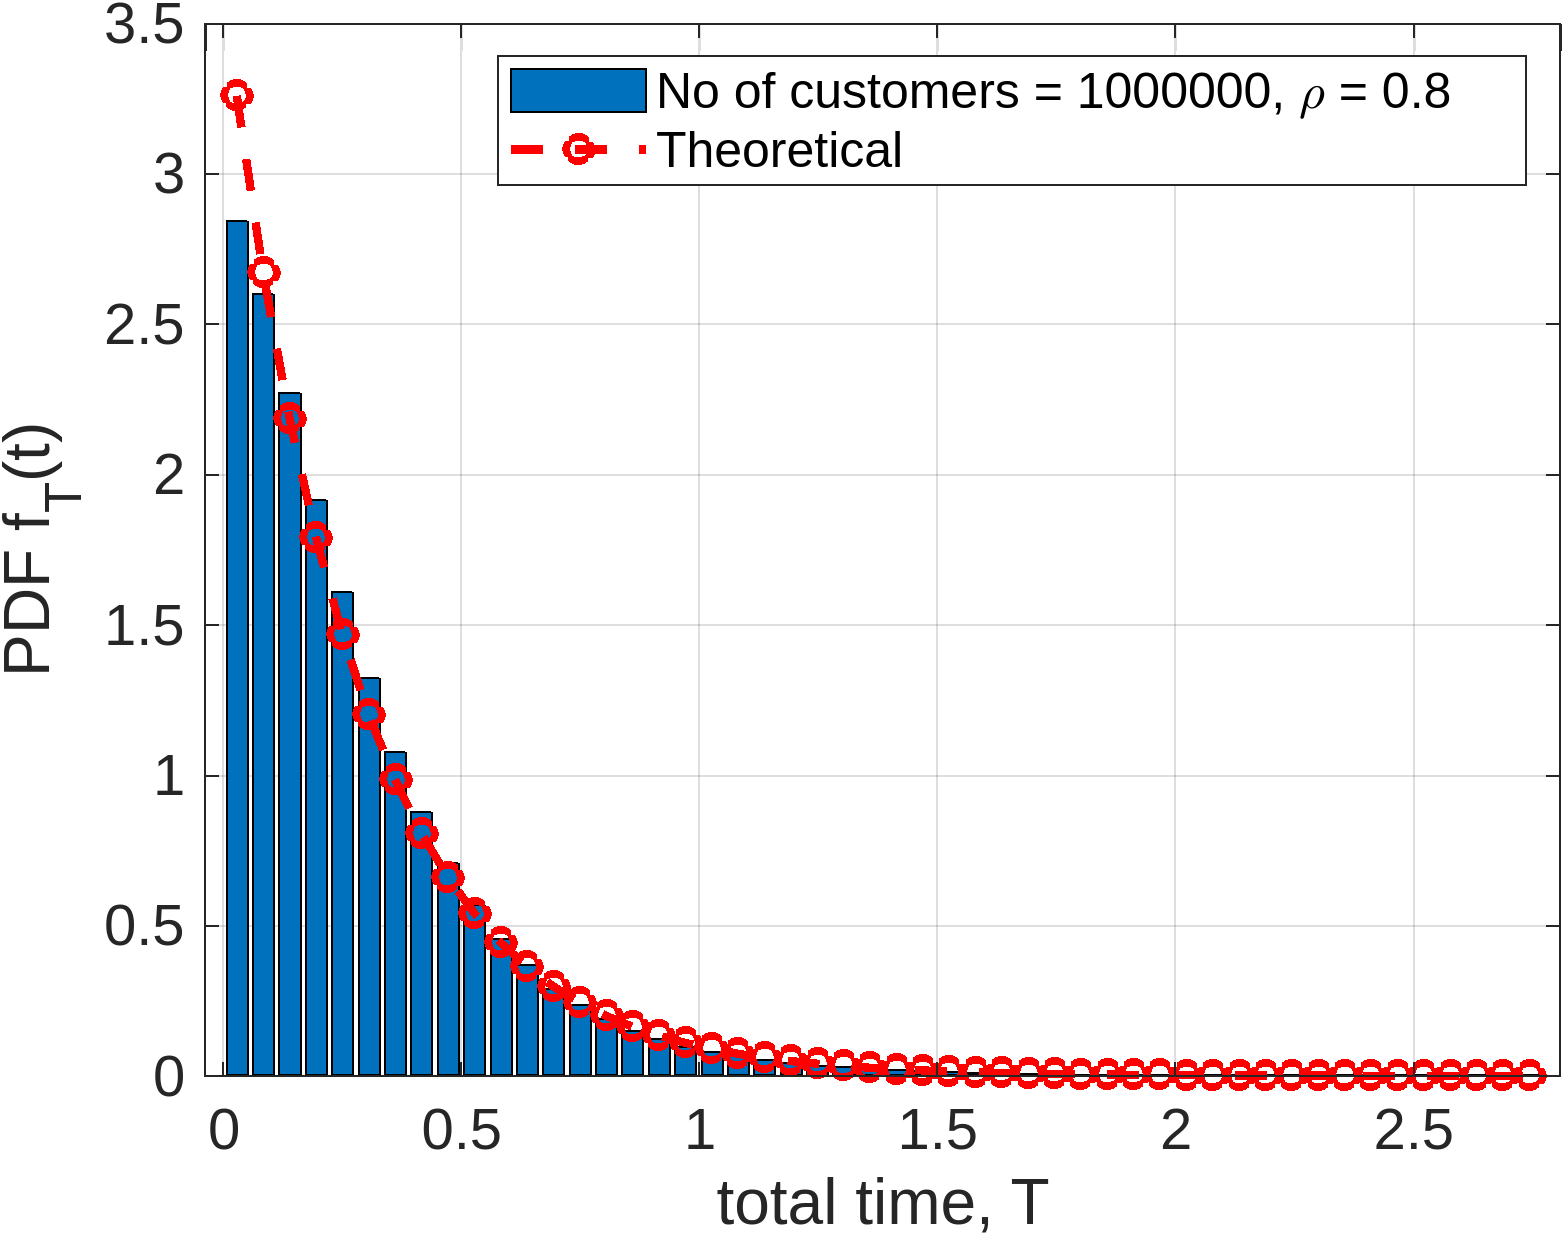
\includegraphics[width=200px]{../code/figures/total_time_dist/bars_plot_no_customers_1000000_rho_0.8.png}
  }
  \subfloat[]{
    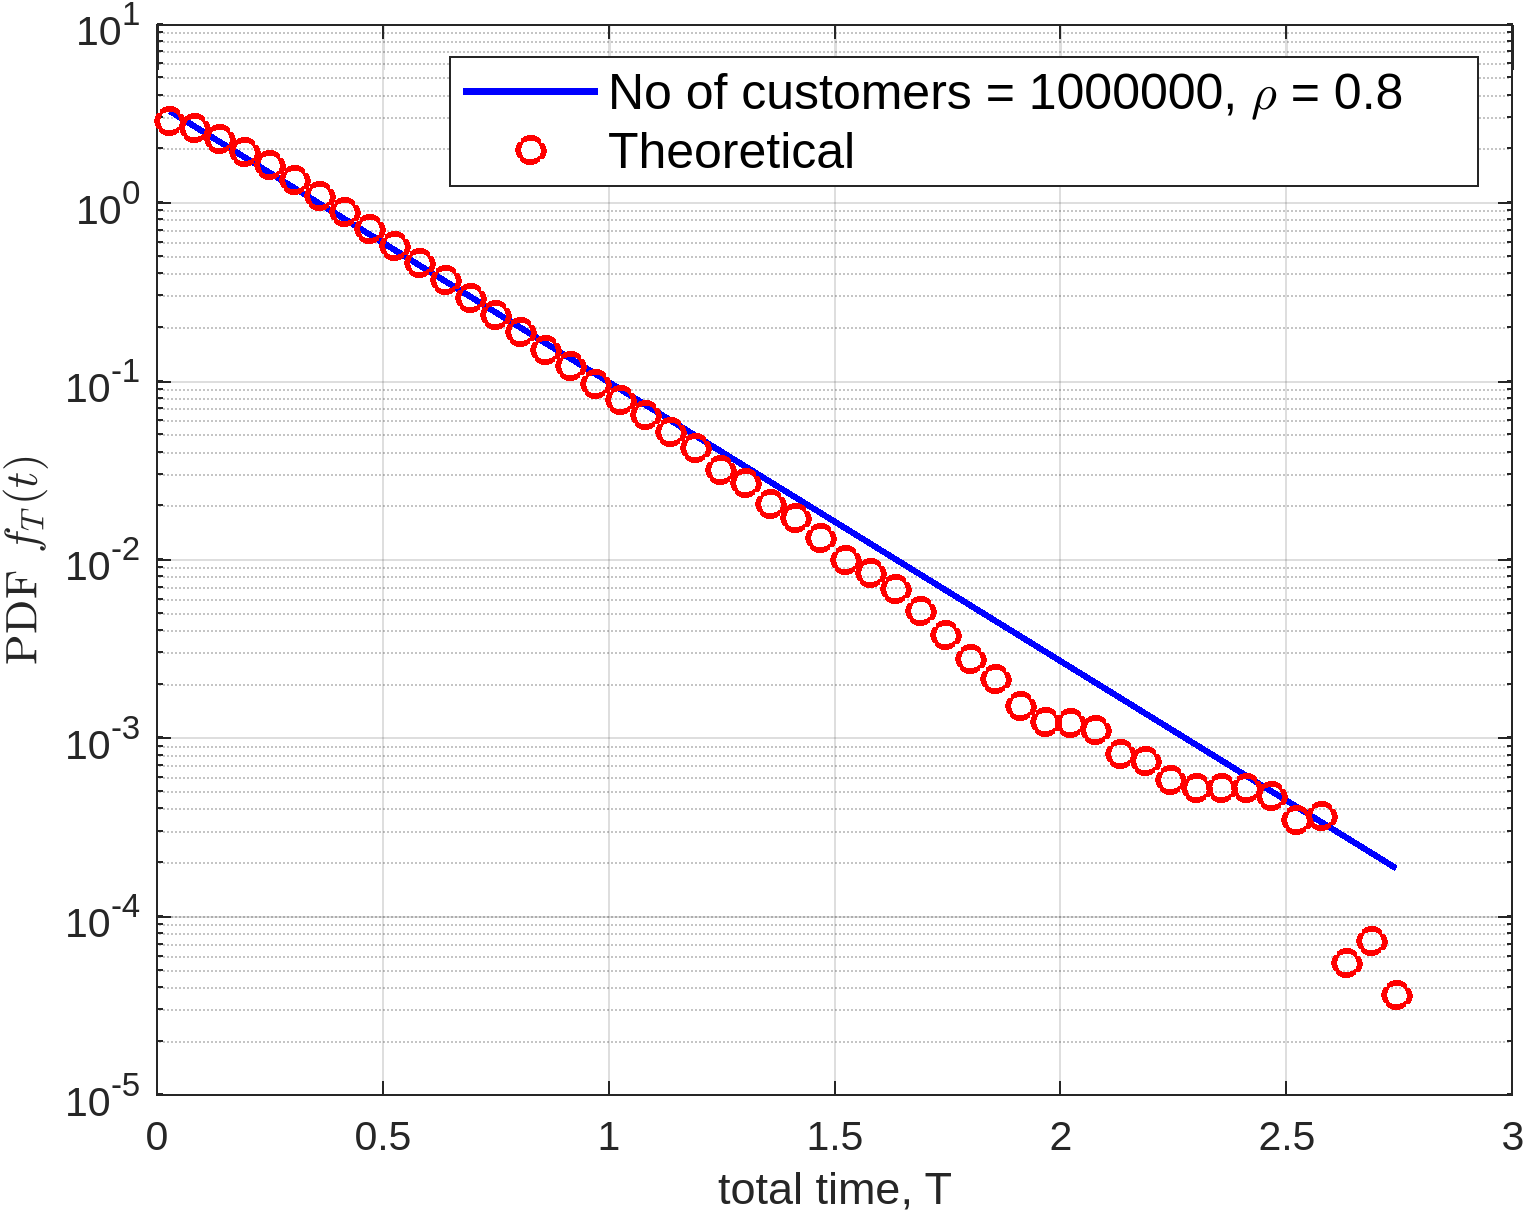
\includegraphics[width=200px]{../code/figures/total_time_dist/semilogy_plot_no_customers_1000000_rho_0.8.png}
  }
  \hspace{0px}
  \subfloat[]{
    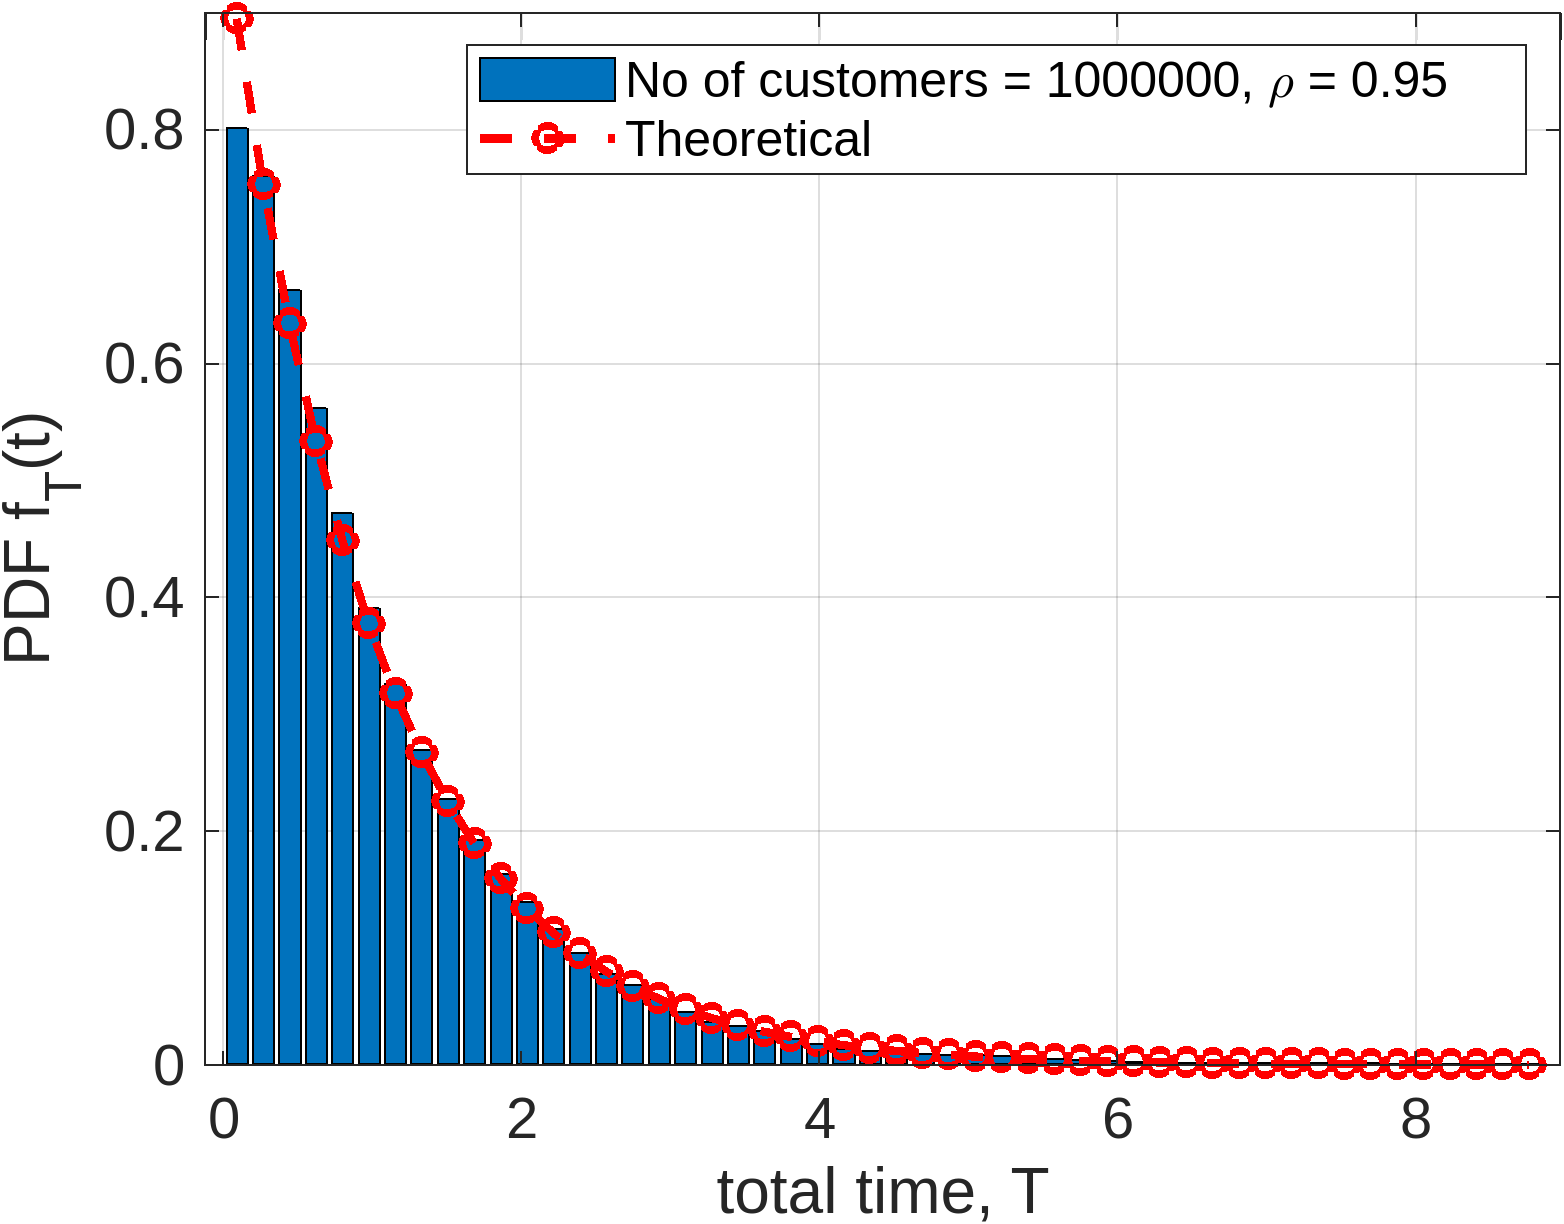
\includegraphics[width=200px]{../code/figures/total_time_dist/bars_plot_no_customers_1000000_rho_0.95.png}
  }
  \subfloat[]{
    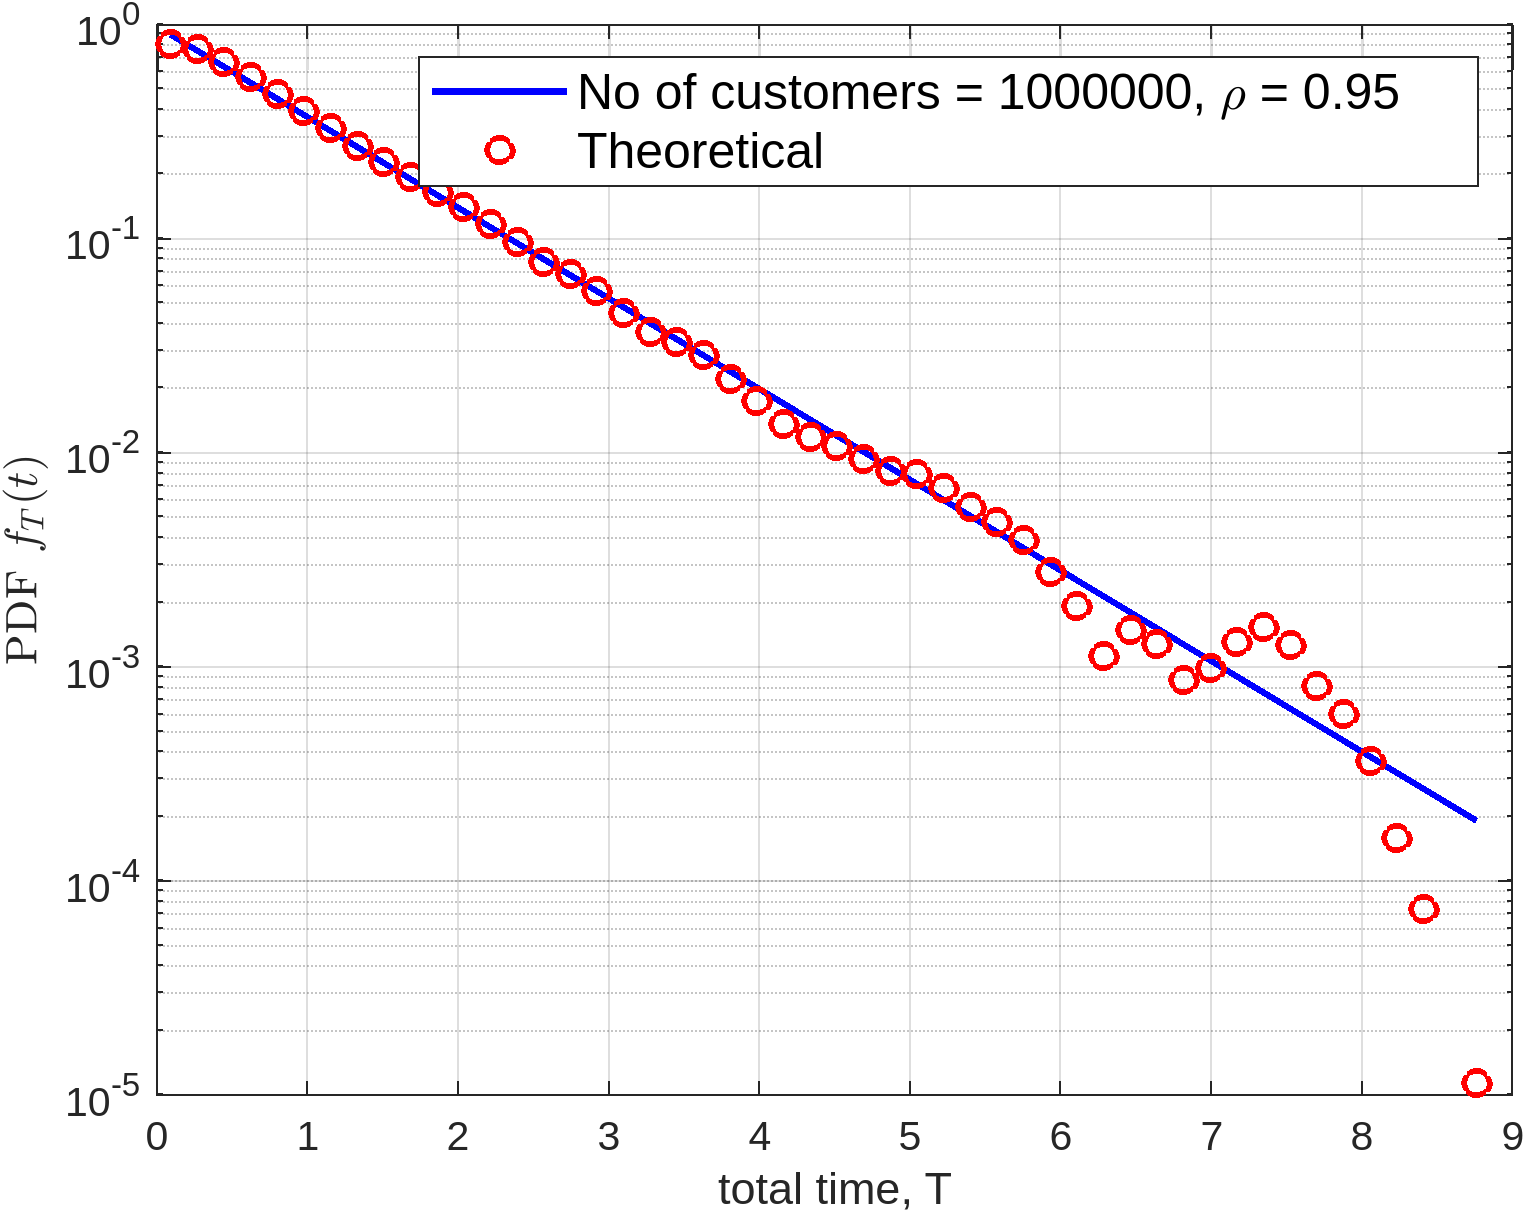
\includegraphics[width=200px]{../code/figures/total_time_dist/semilogy_plot_no_customers_1000000_rho_0.95.png}
  }
  \caption{PDF of the total time in the system for high $\rho$ and $1000000$ customers}  
  \label{PDF_TT_high_more_cus}
\end{figure}

\subsection{PDF of the waiting time}
\begin{figure}[H]
  \centering
  \subfloat[]{
    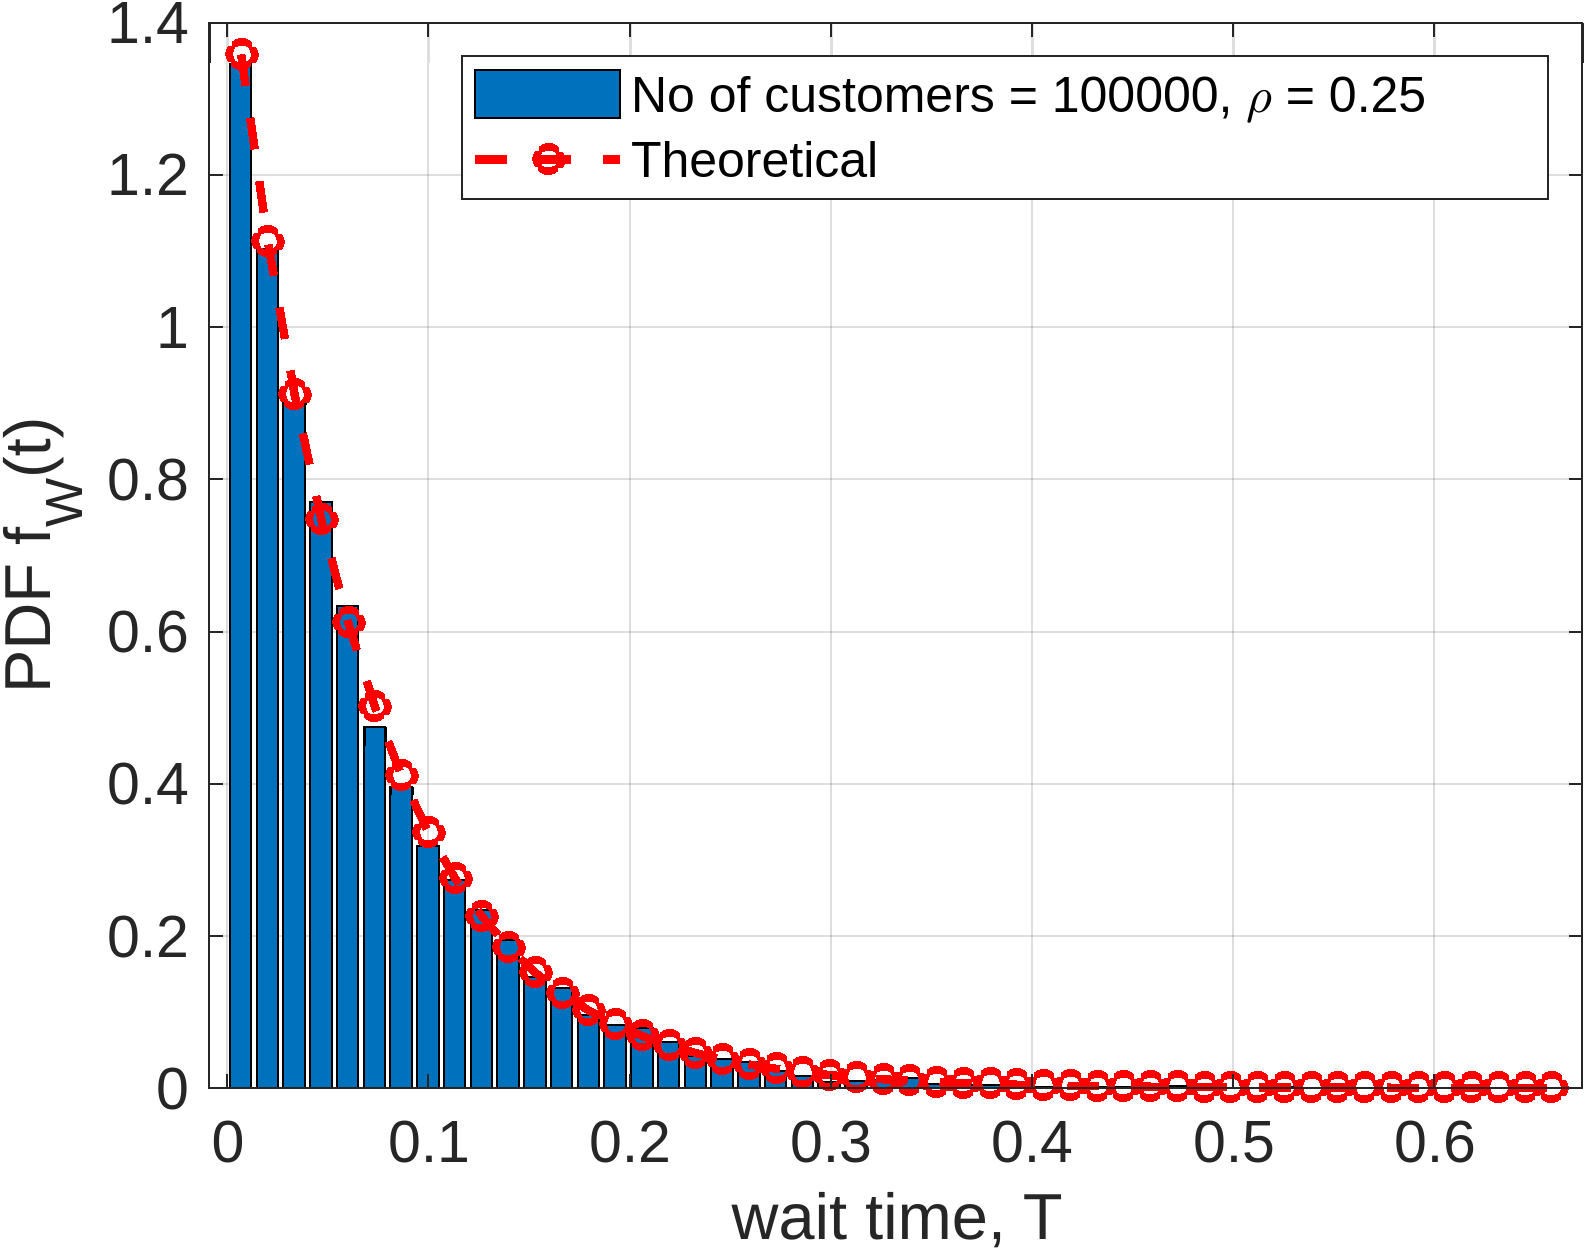
\includegraphics[width=200px]{../code/figures/waiting_time_dist/bar_plot_no_customers_100000_rho_0.25.png}
  }
  \subfloat[]{
    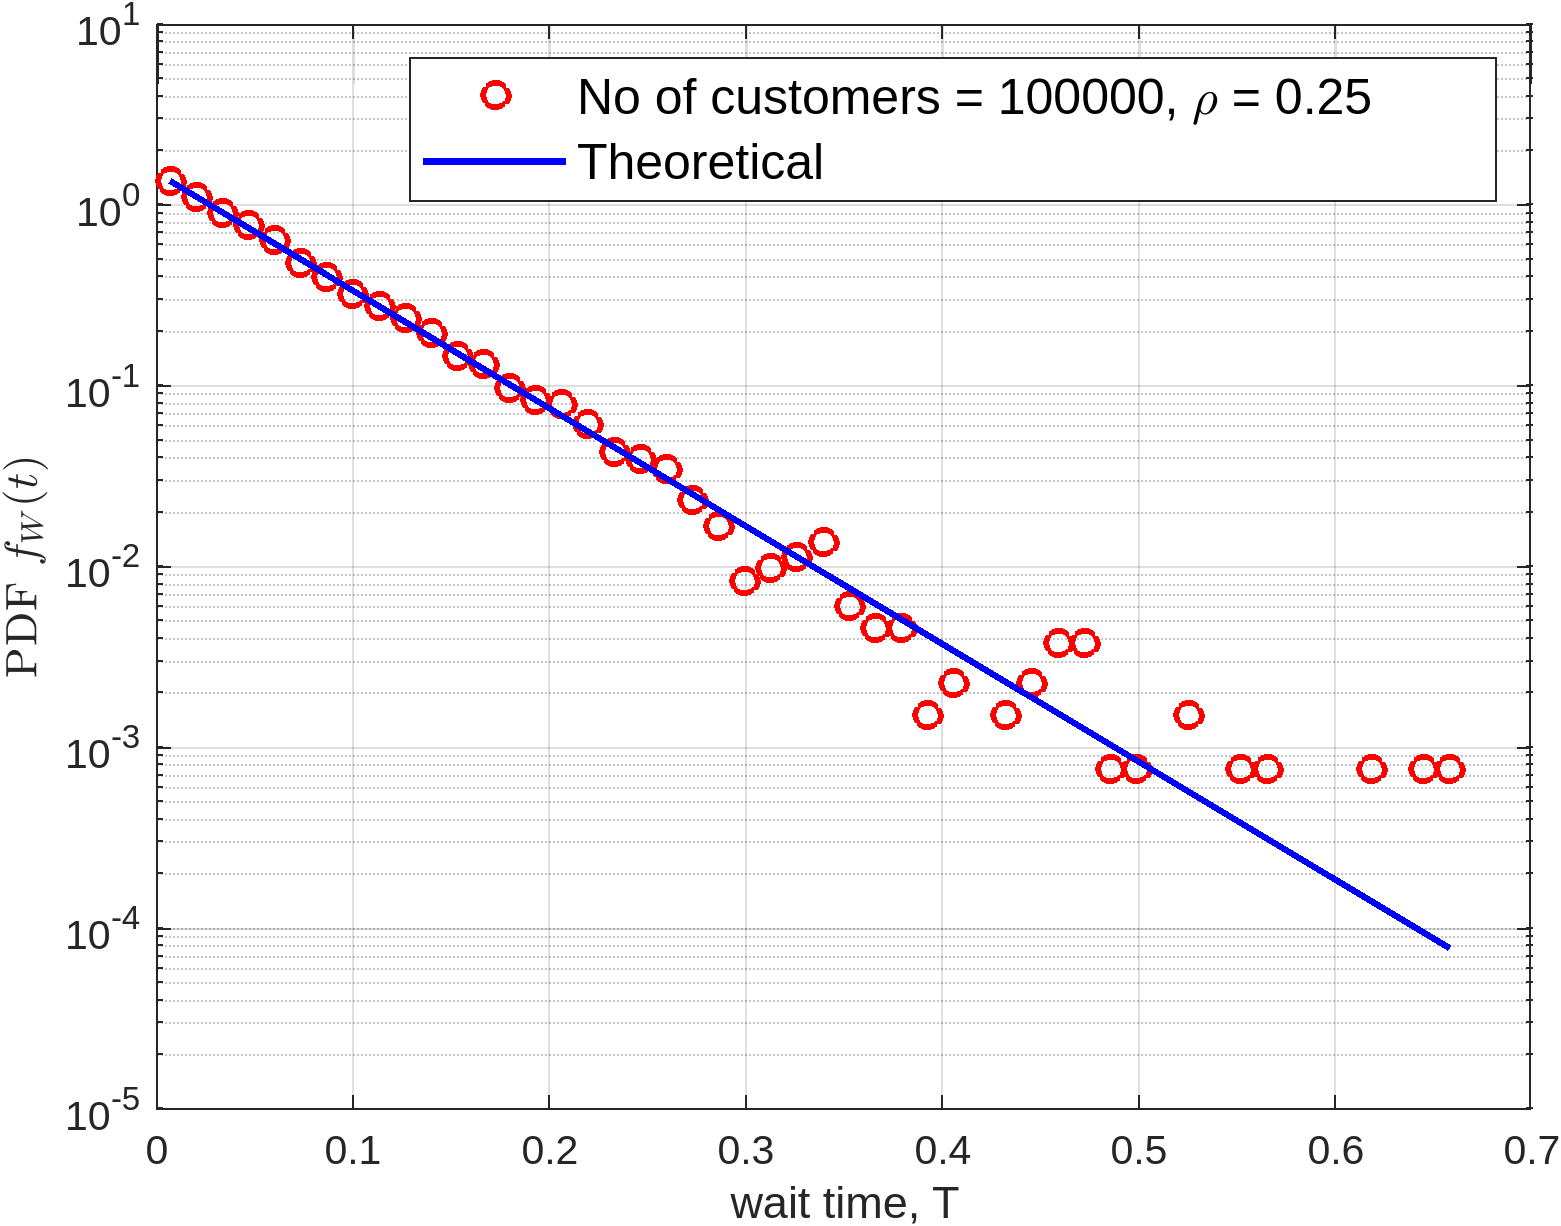
\includegraphics[width=200px]{../code/figures/waiting_time_dist/semilogy_plot_no_customers_100000_rho_0.25.png}
  }
  \hspace{0px}
  \subfloat[]{
    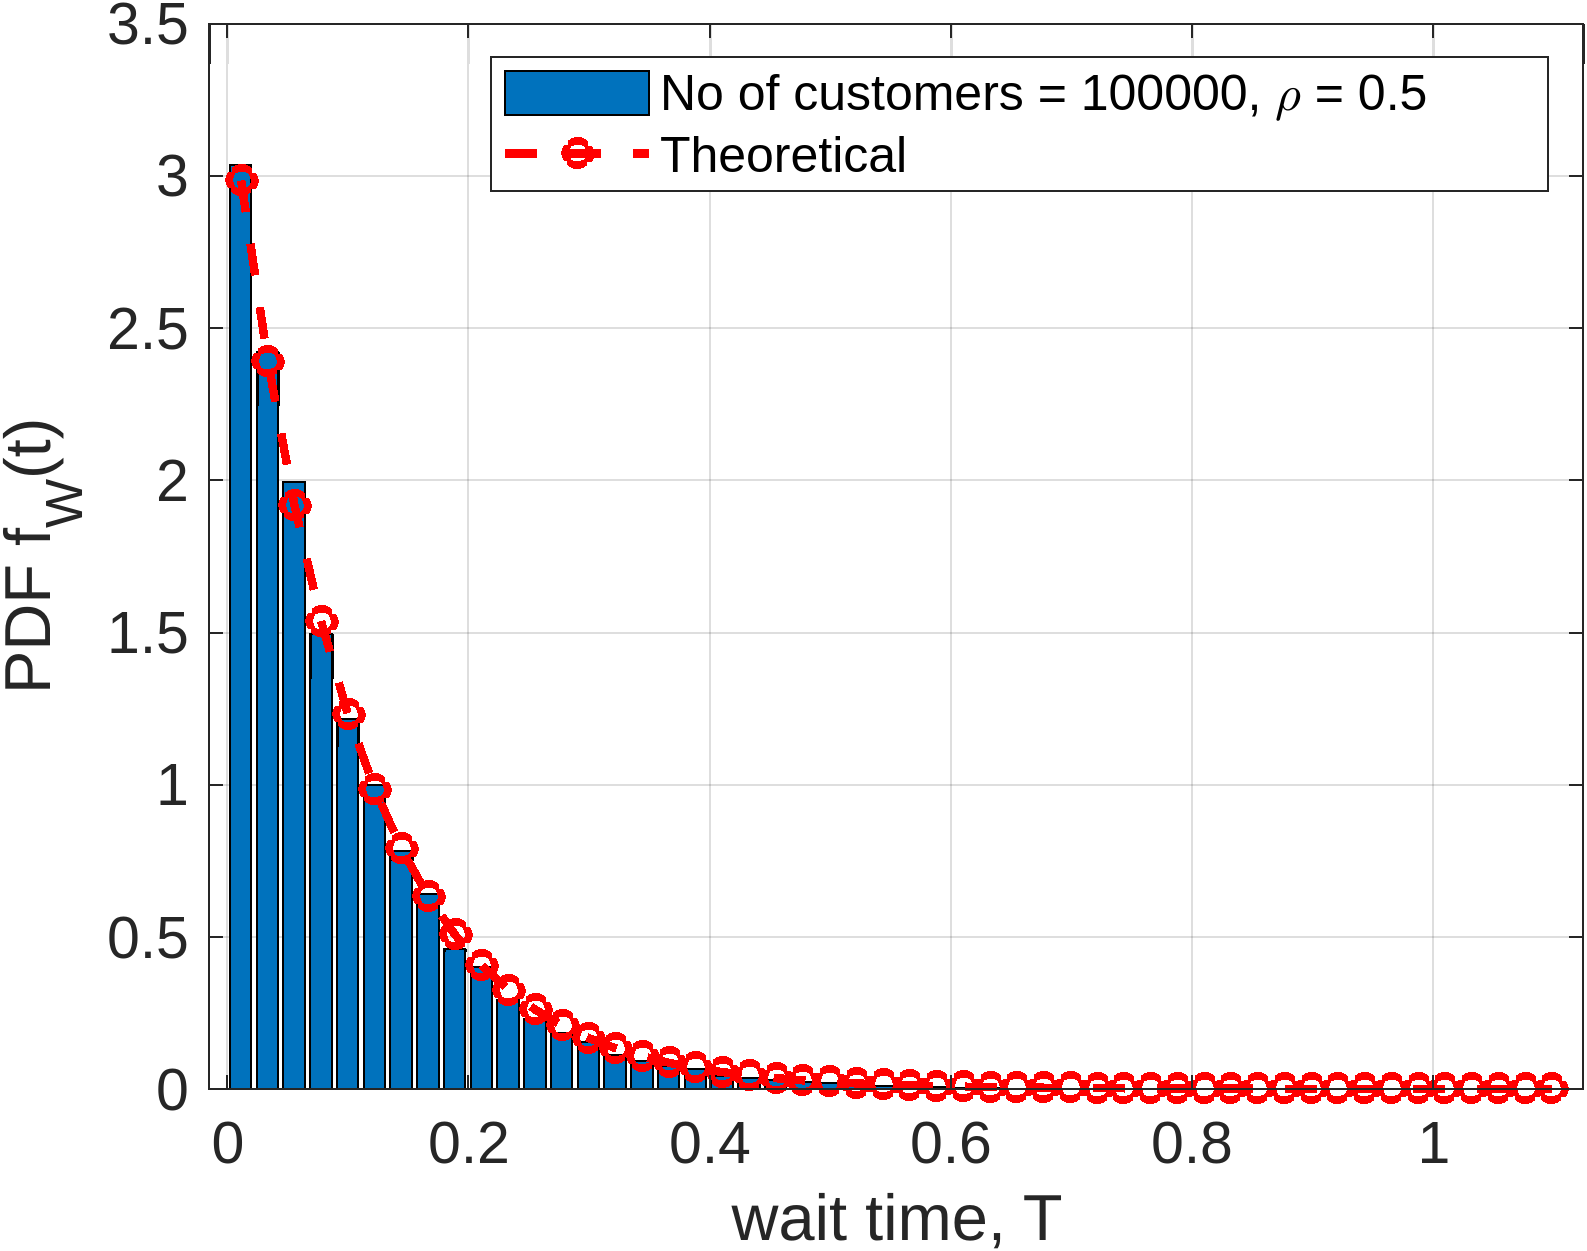
\includegraphics[width=200px]{../code/figures/waiting_time_dist/bar_plot_no_customers_100000_rho_0.5.png}
  }
  \subfloat[]{
    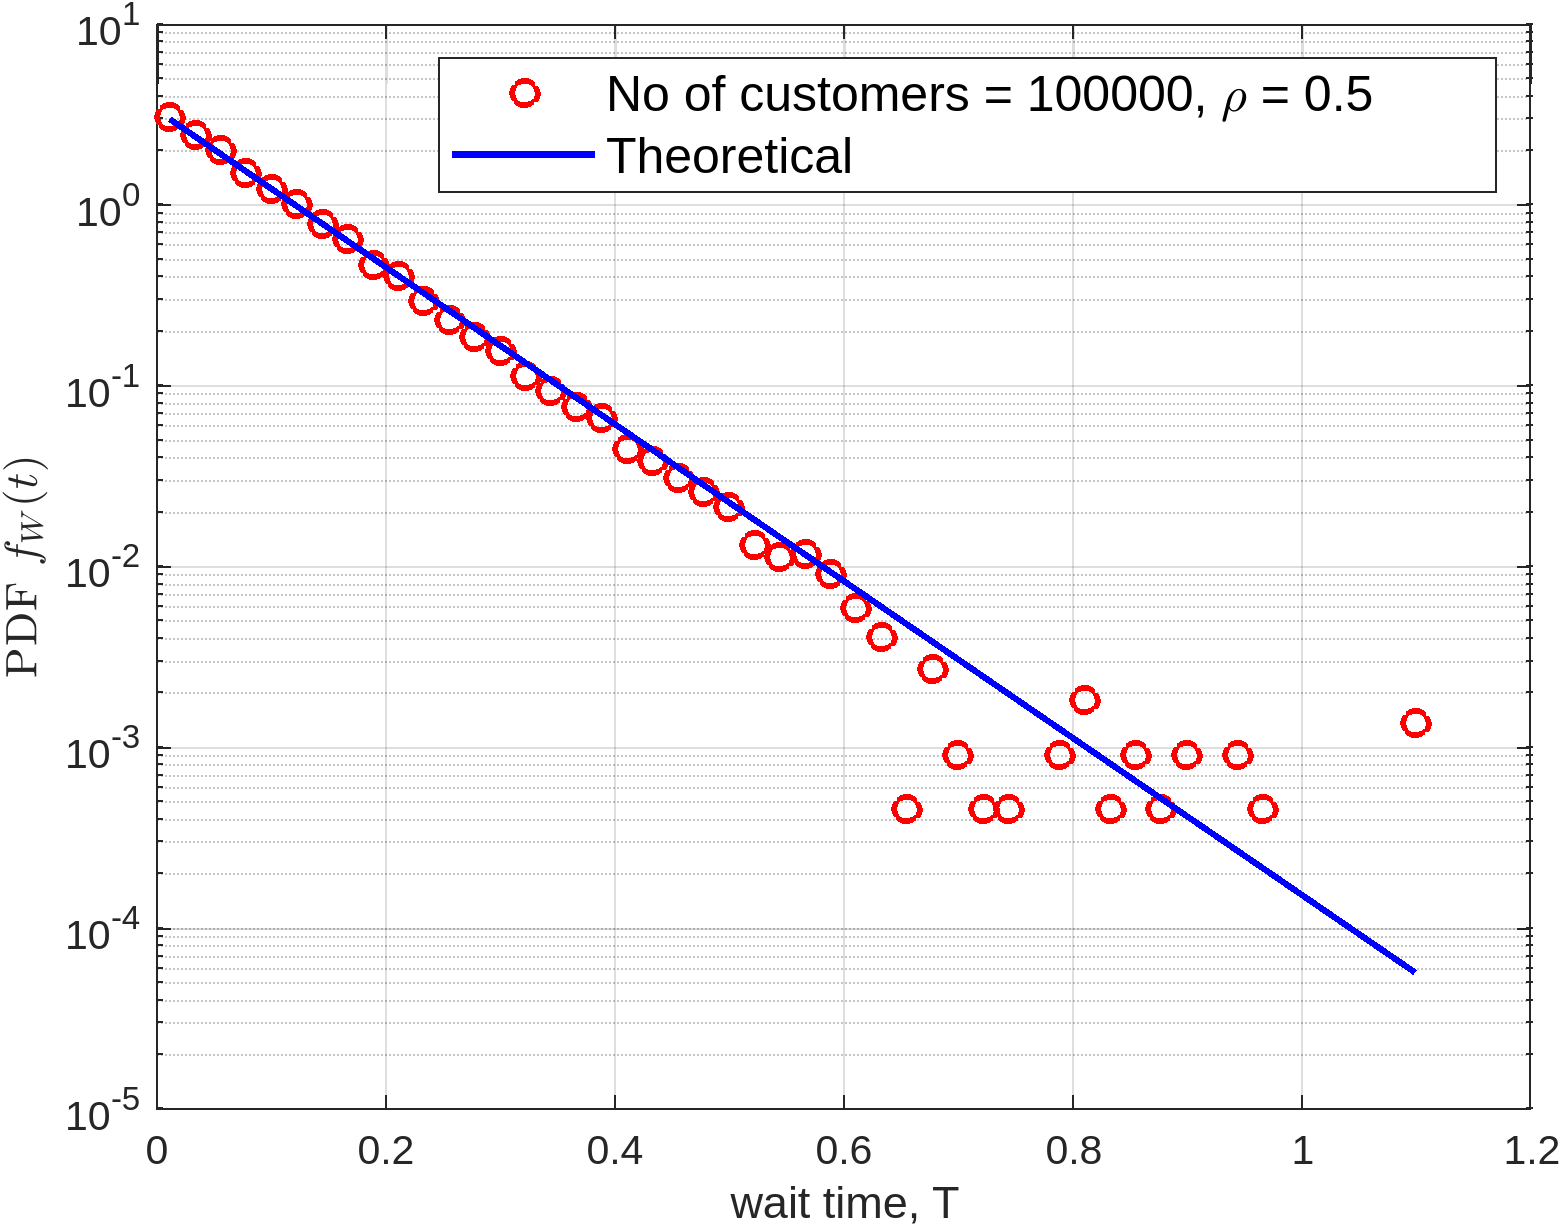
\includegraphics[width=200px]{../code/figures/waiting_time_dist/semilogy_plot_no_customers_100000_rho_0.5.png}
  }
  \caption{PDF of the waiting time in the system for low and medium $\rho$}  
  \label{PDF_W_low_med}
\end{figure}

\begin{figure}[H]
  \centering
  \subfloat[]{
    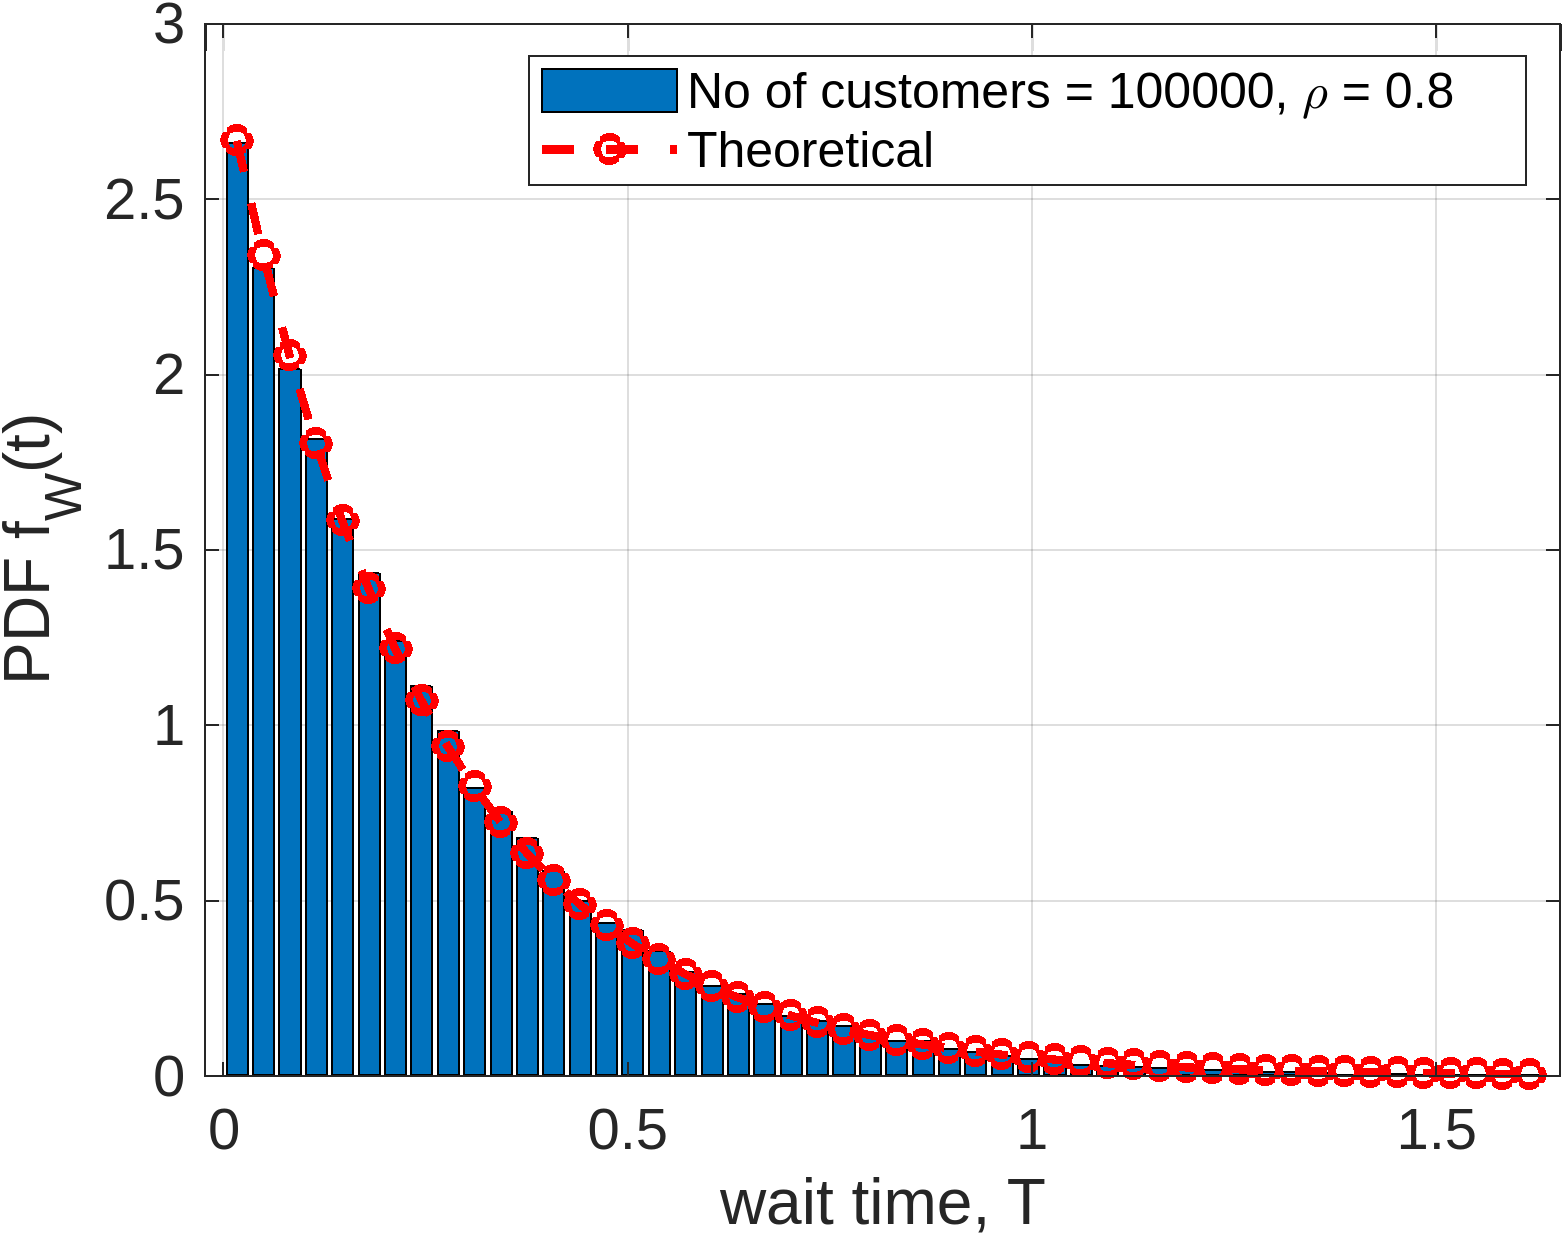
\includegraphics[width=200px]{../code/figures/waiting_time_dist/bar_plot_no_customers_100000_rho_0.8.png}
  }
  \subfloat[]{
    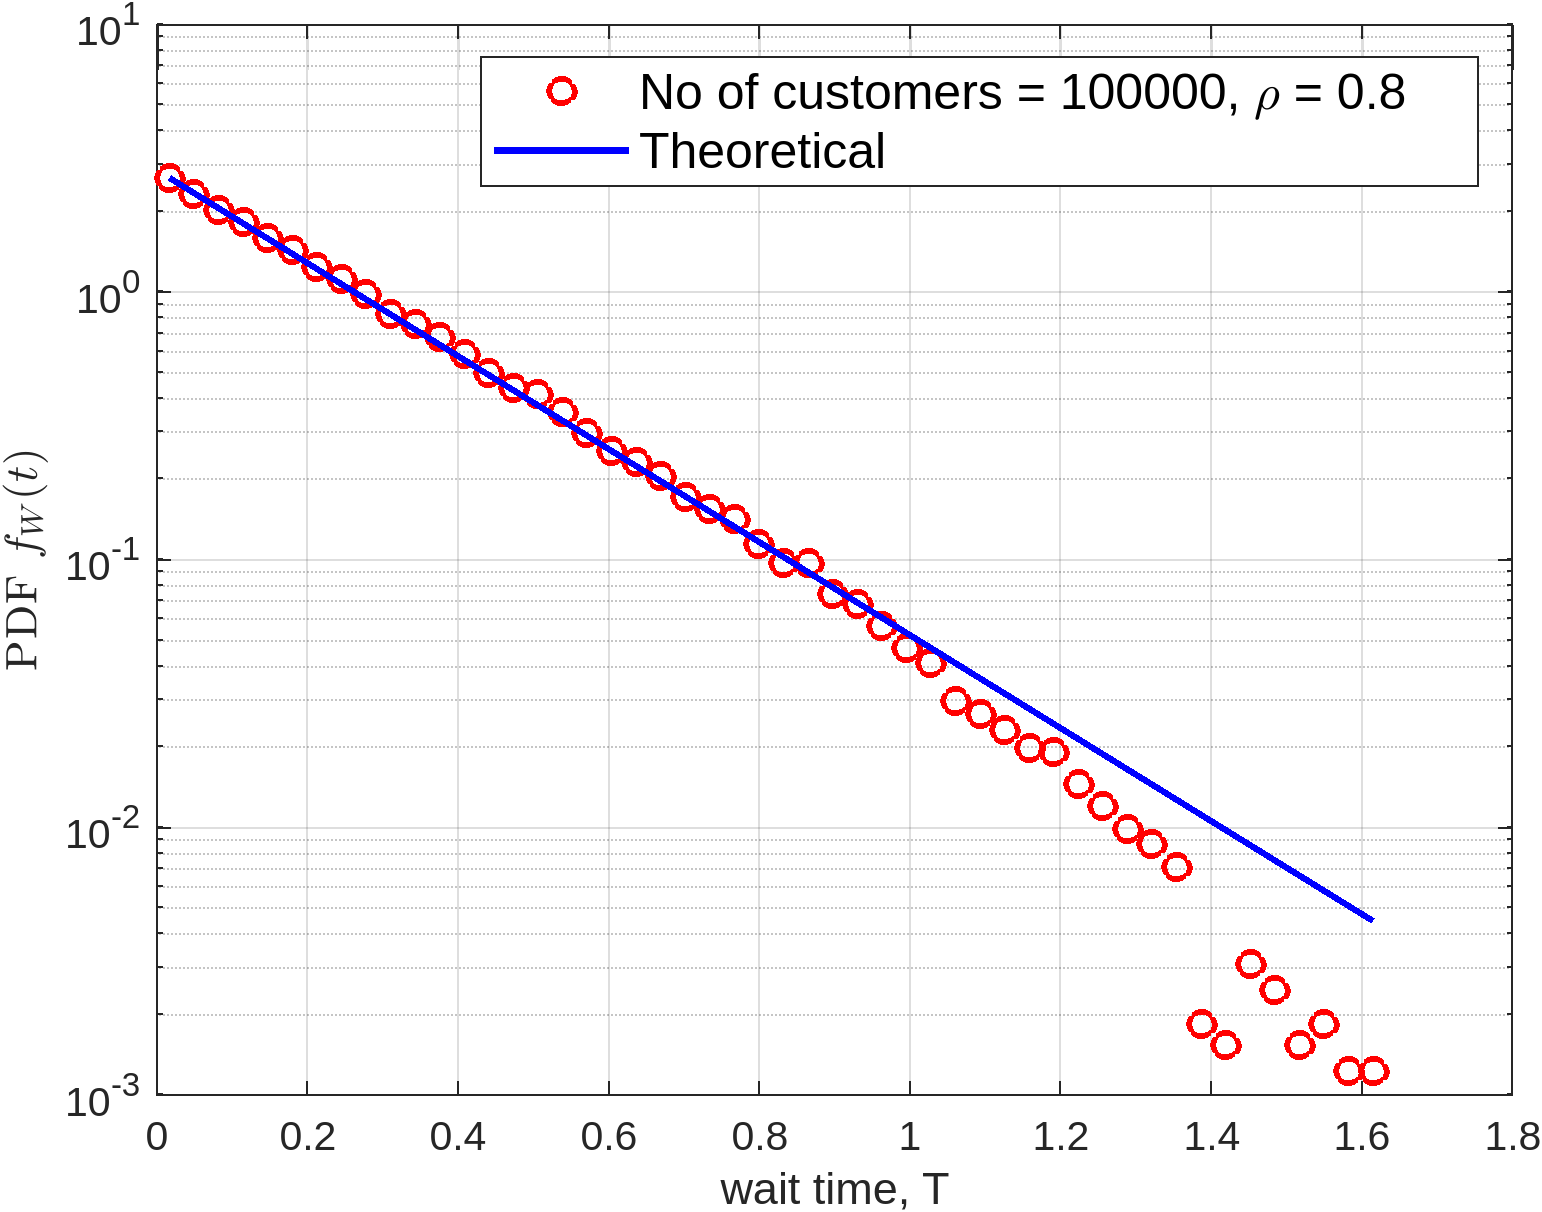
\includegraphics[width=200px]{../code/figures/waiting_time_dist/semilogy_plot_no_customers_100000_rho_0.8.png}
  }
  \hspace{0px}
  \subfloat[]{
    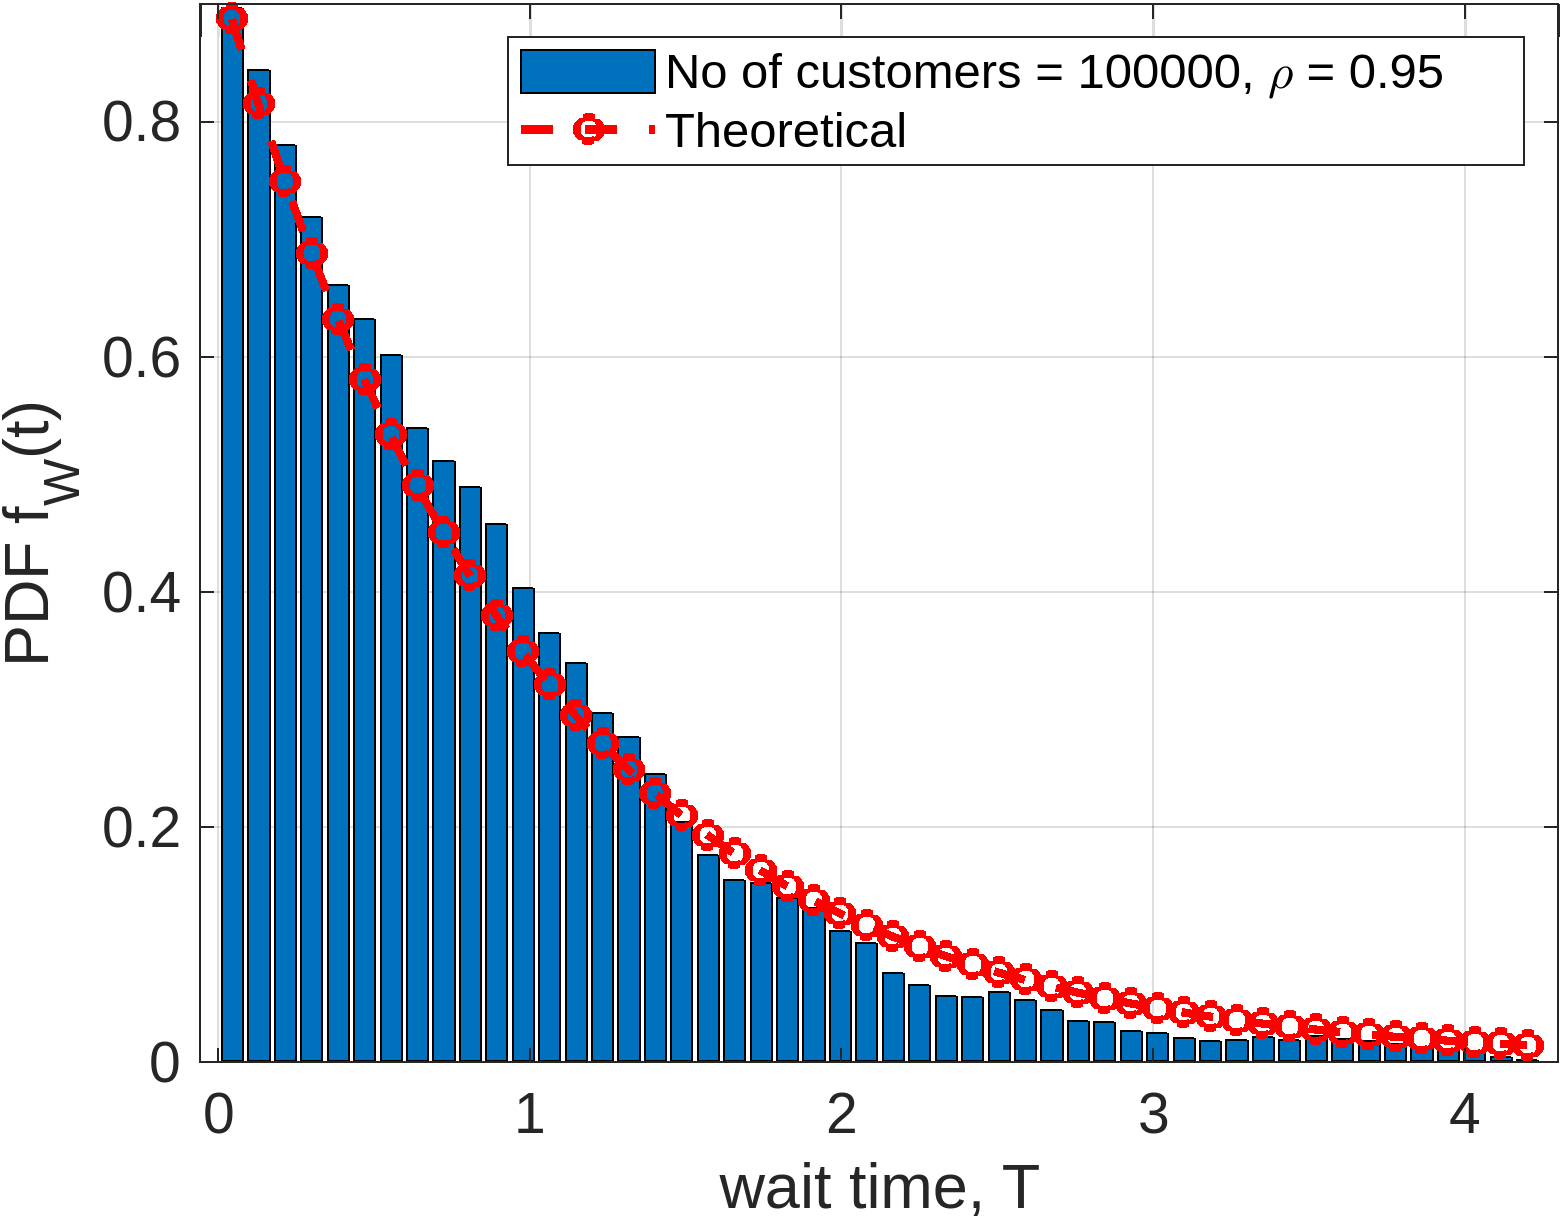
\includegraphics[width=200px]{../code/figures/waiting_time_dist/bar_plot_no_customers_100000_rho_0.95.png}
  }
  \subfloat[]{
    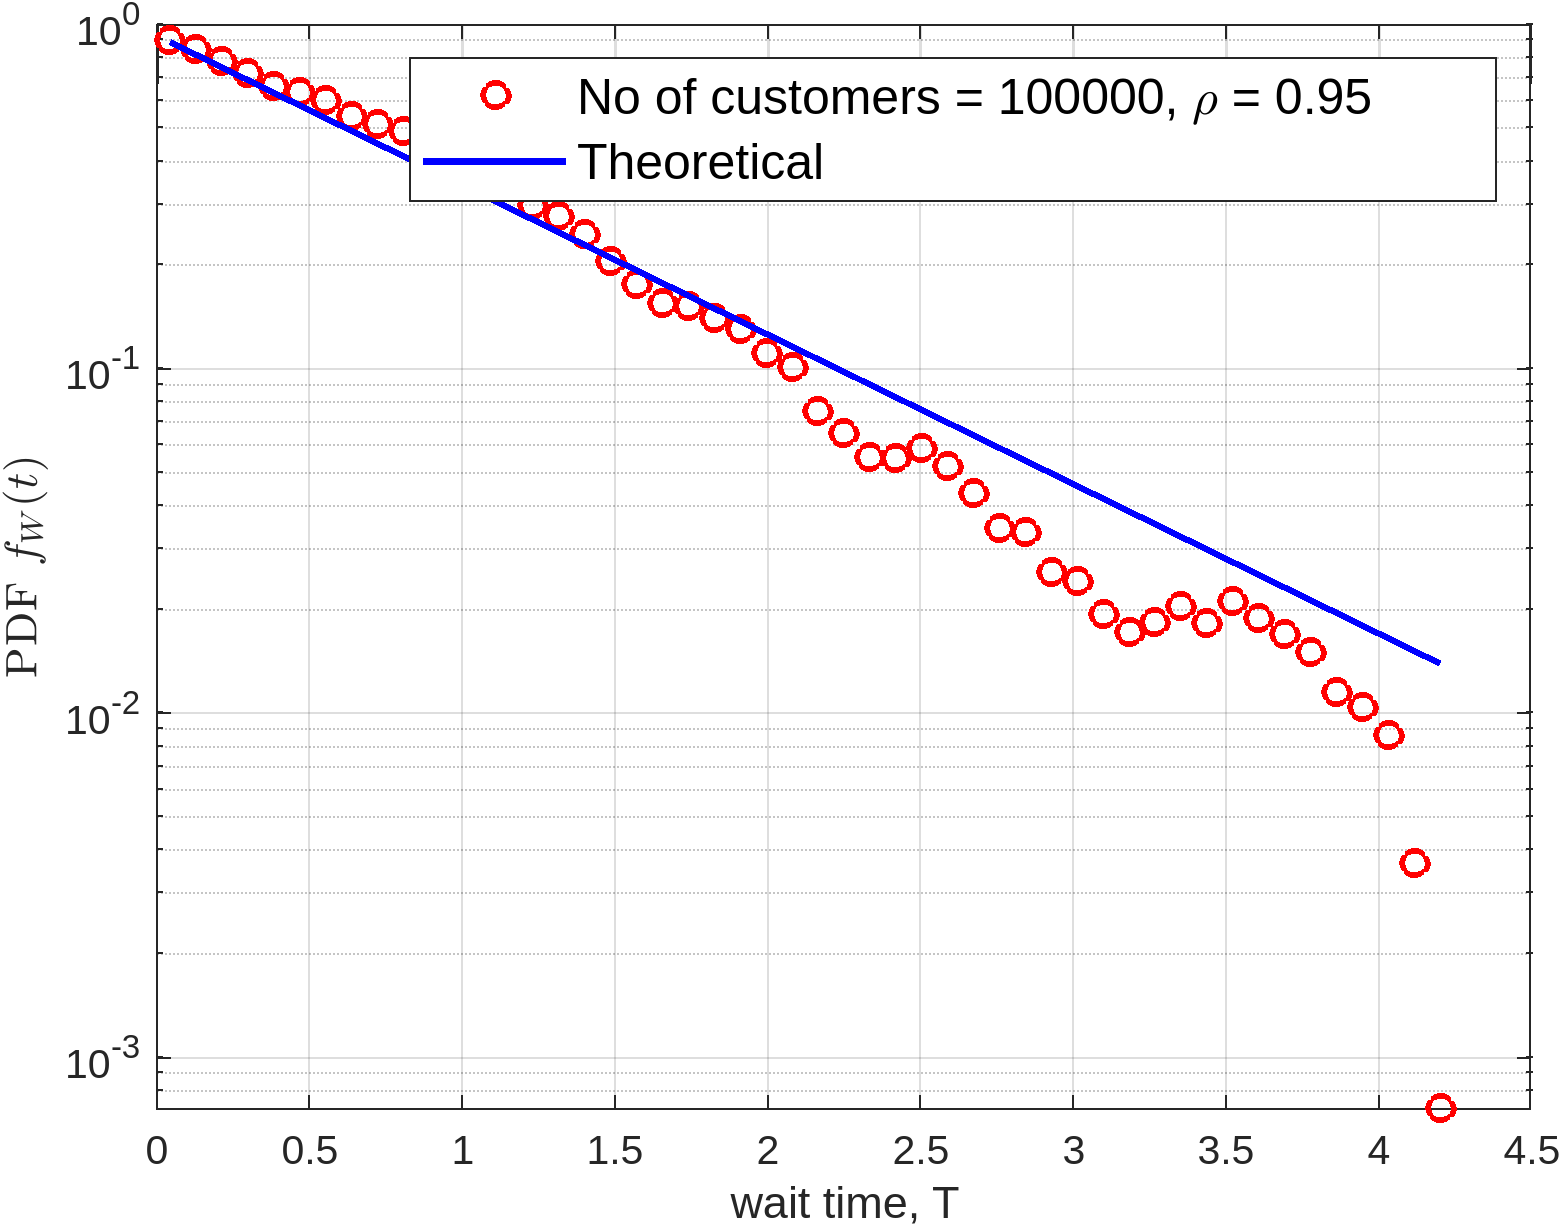
\includegraphics[width=200px]{../code/figures/waiting_time_dist/semilogy_plot_no_customers_100000_rho_0.95.png}
  }
  \caption{PDF of the waiting time in the system for high $\rho$}  
  \label{PDF_W_high}
\end{figure}

Figure \ref{PDF_W_low_med} shows the PDF of the waiting time for low traffic intensity, $\rho=0.25$
and a medium traffic intensity, $\rho=0.5$. They are exponentially distributed, and they match with
theoretical distributions. Figure \ref{PDF_W_high} indicates the distribution of the waiting time
for high intensities $\rho =0.8$ and $\rho=0.95$. The plot for $\rho=0.8$ is in relatively excellent 
agreement with the theoretical one, but the plot for $\rho =0.95$ is slightly far from the theoretical 
PDF. We have increased the number of customers for the high intensity cases to $1000000$ customers
and the results have improved as shown in Figure \ref{PDF_W_high_more_cust}.

\begin{figure}[H]
  \centering
  \subfloat[]{
    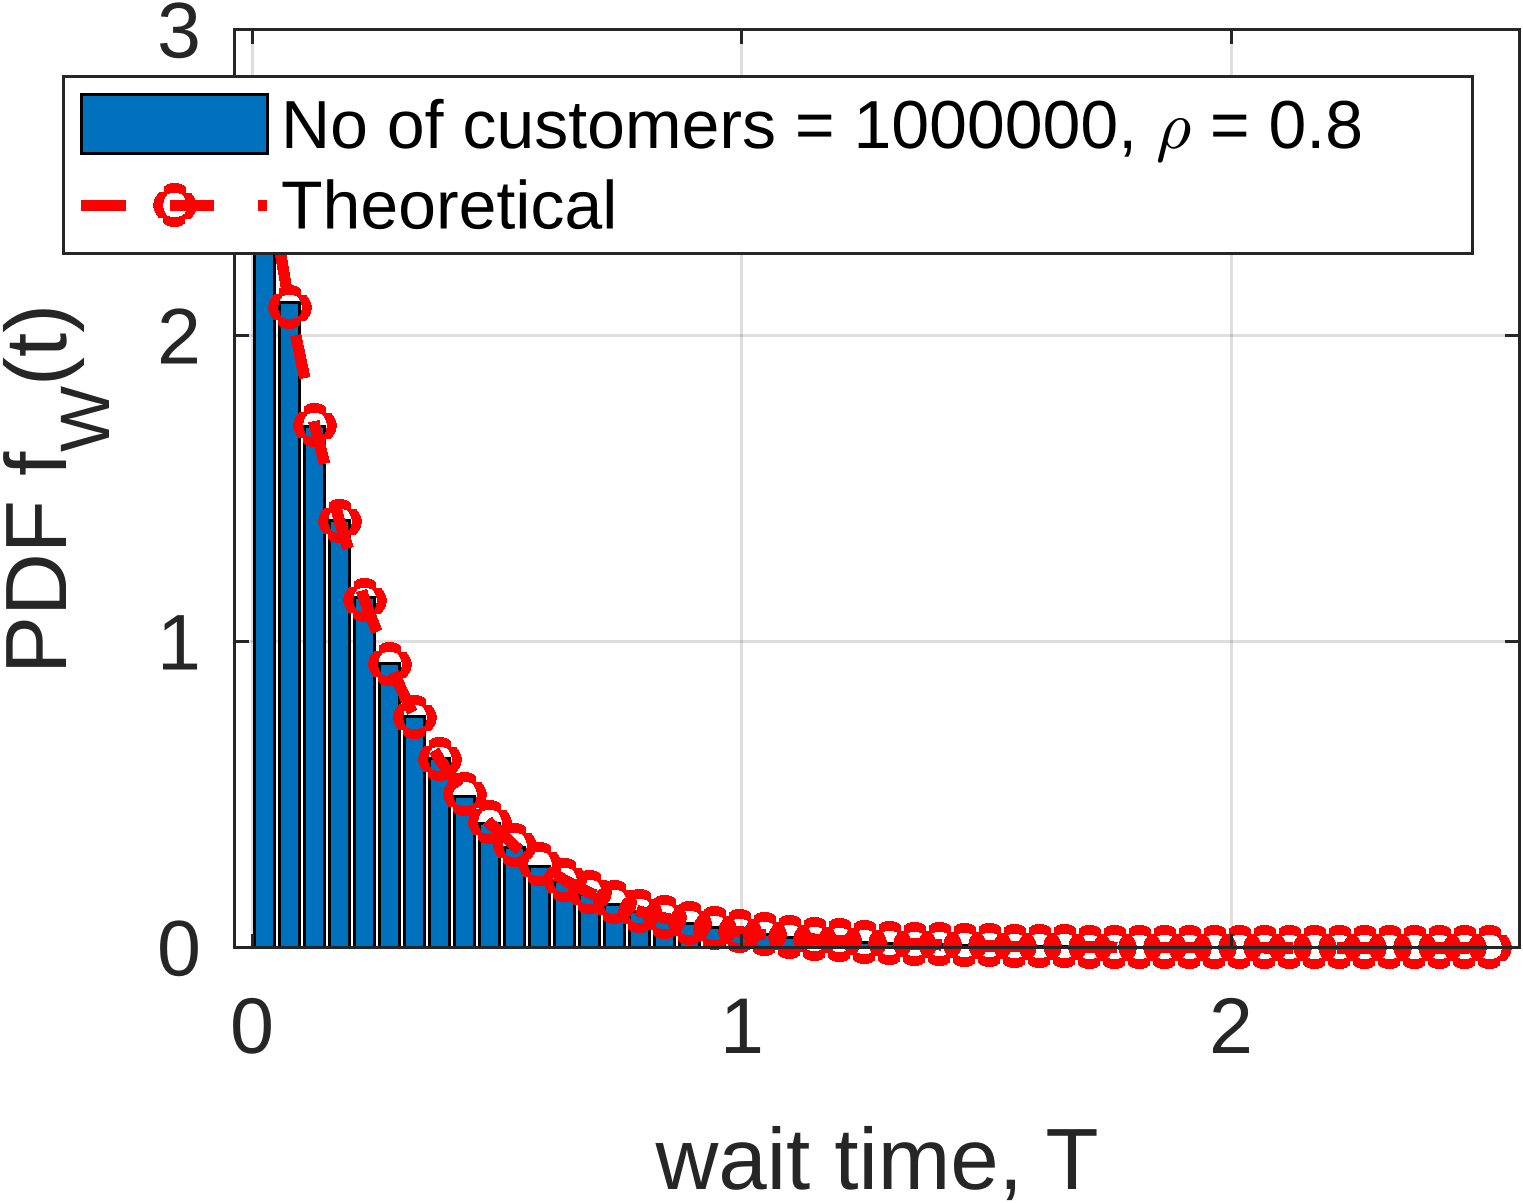
\includegraphics[width=200px]{../code/figures/waiting_time_dist/bar_plot_no_customers_1000000_rho_0.8.png}
  }
  \subfloat[]{
    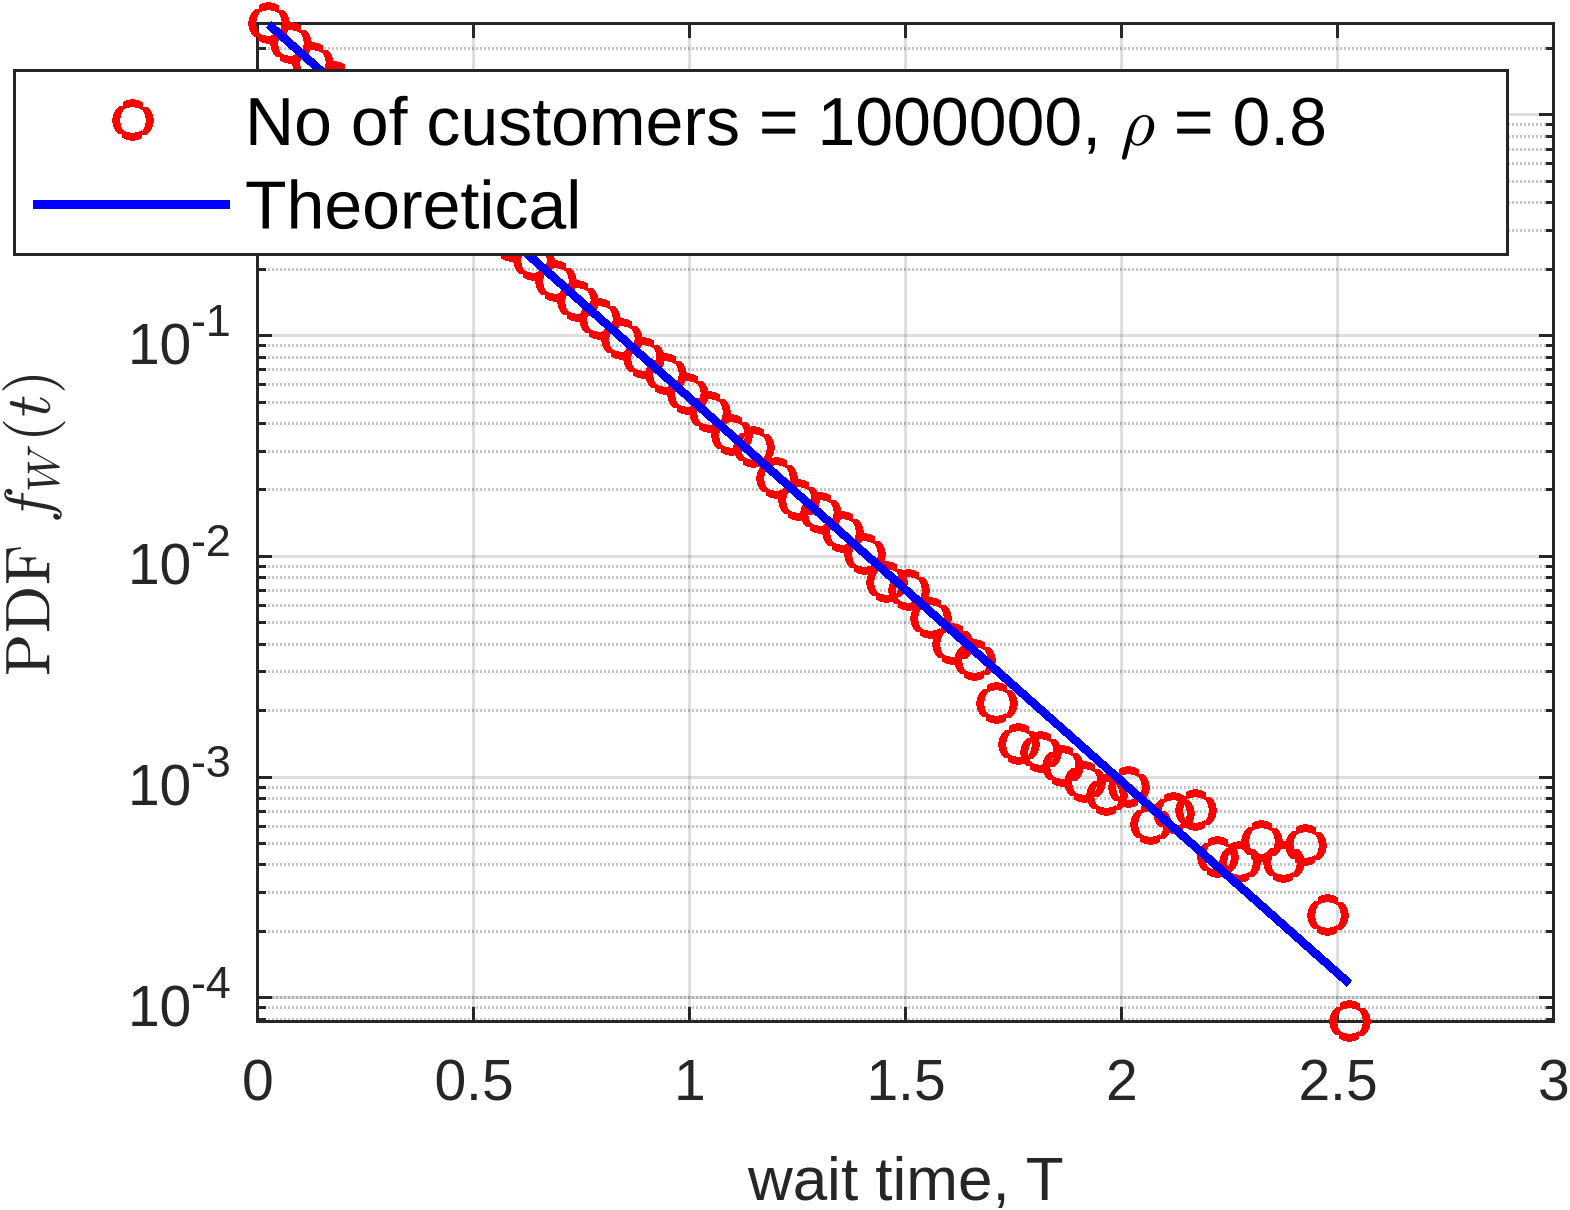
\includegraphics[width=200px]{../code/figures/waiting_time_dist/semilogy_plot_no_customers_1000000_rho_0.8.png}
  }
  \hspace{0px}
  \subfloat[]{
    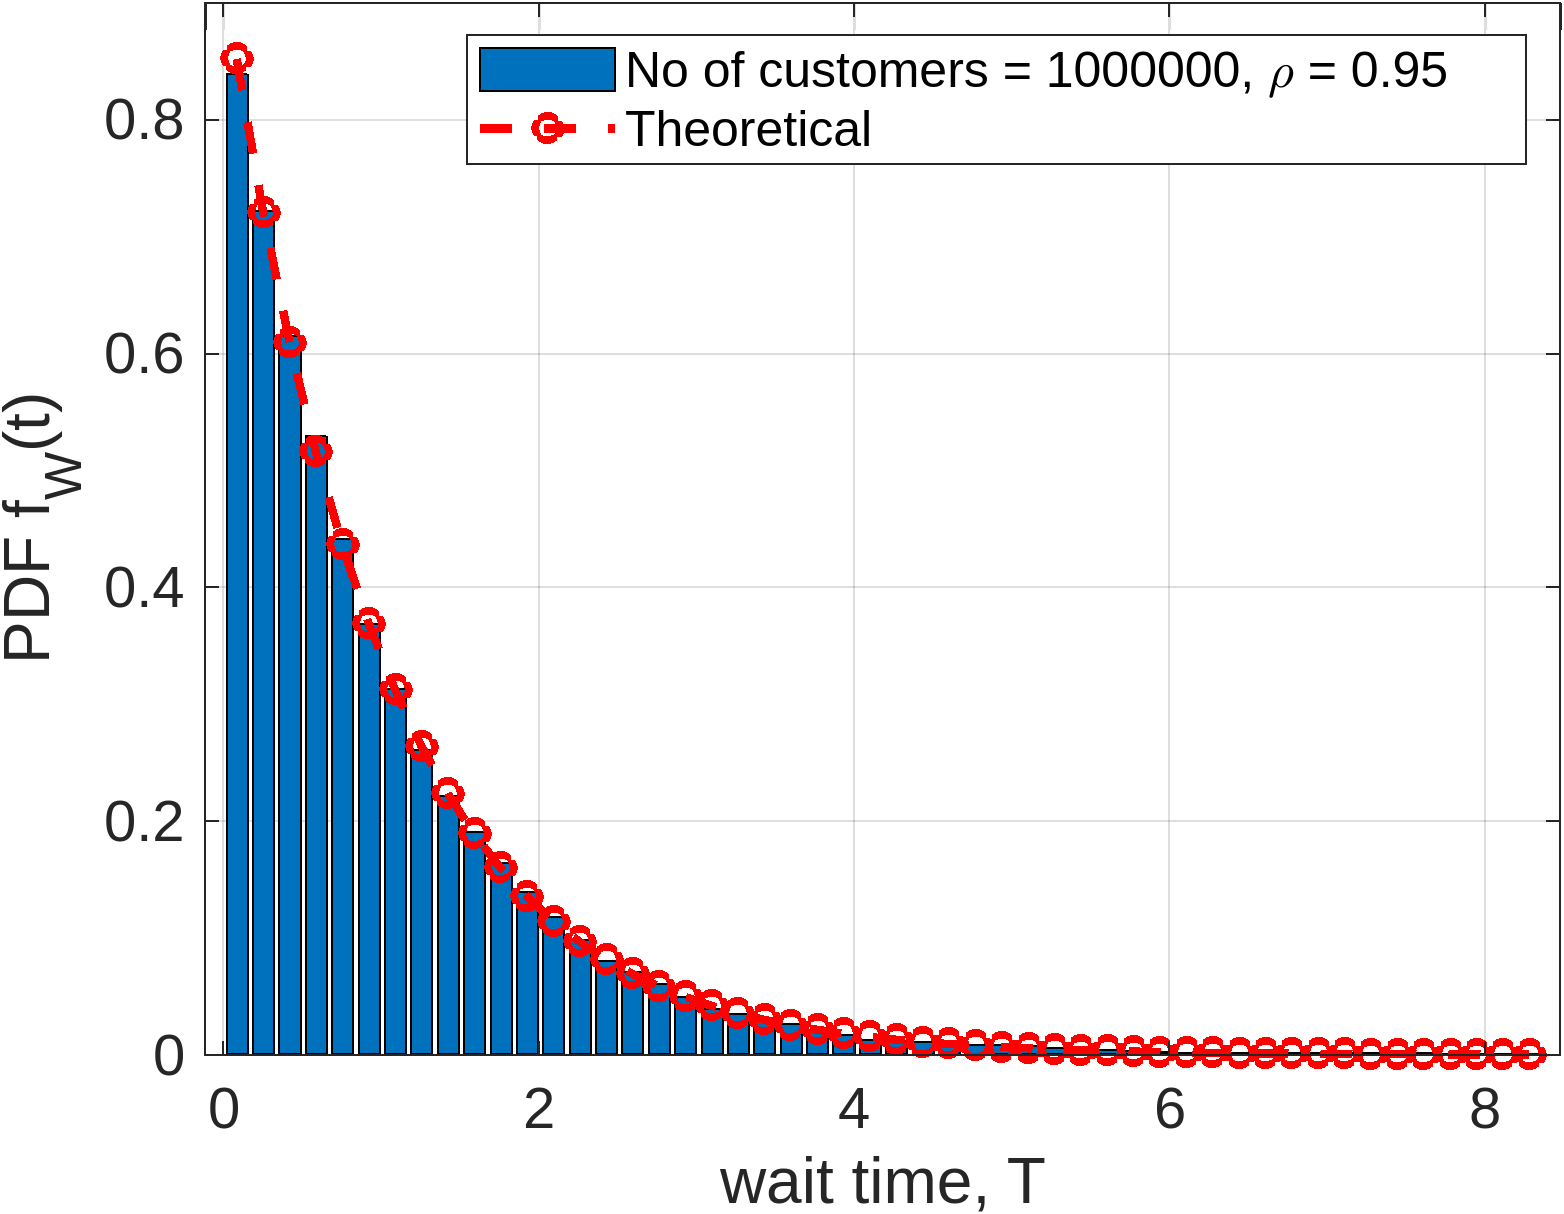
\includegraphics[width=200px]{../code/figures/waiting_time_dist/bar_plot_no_customers_1000000_rho_0.95.png}
  }
  \subfloat[]{
    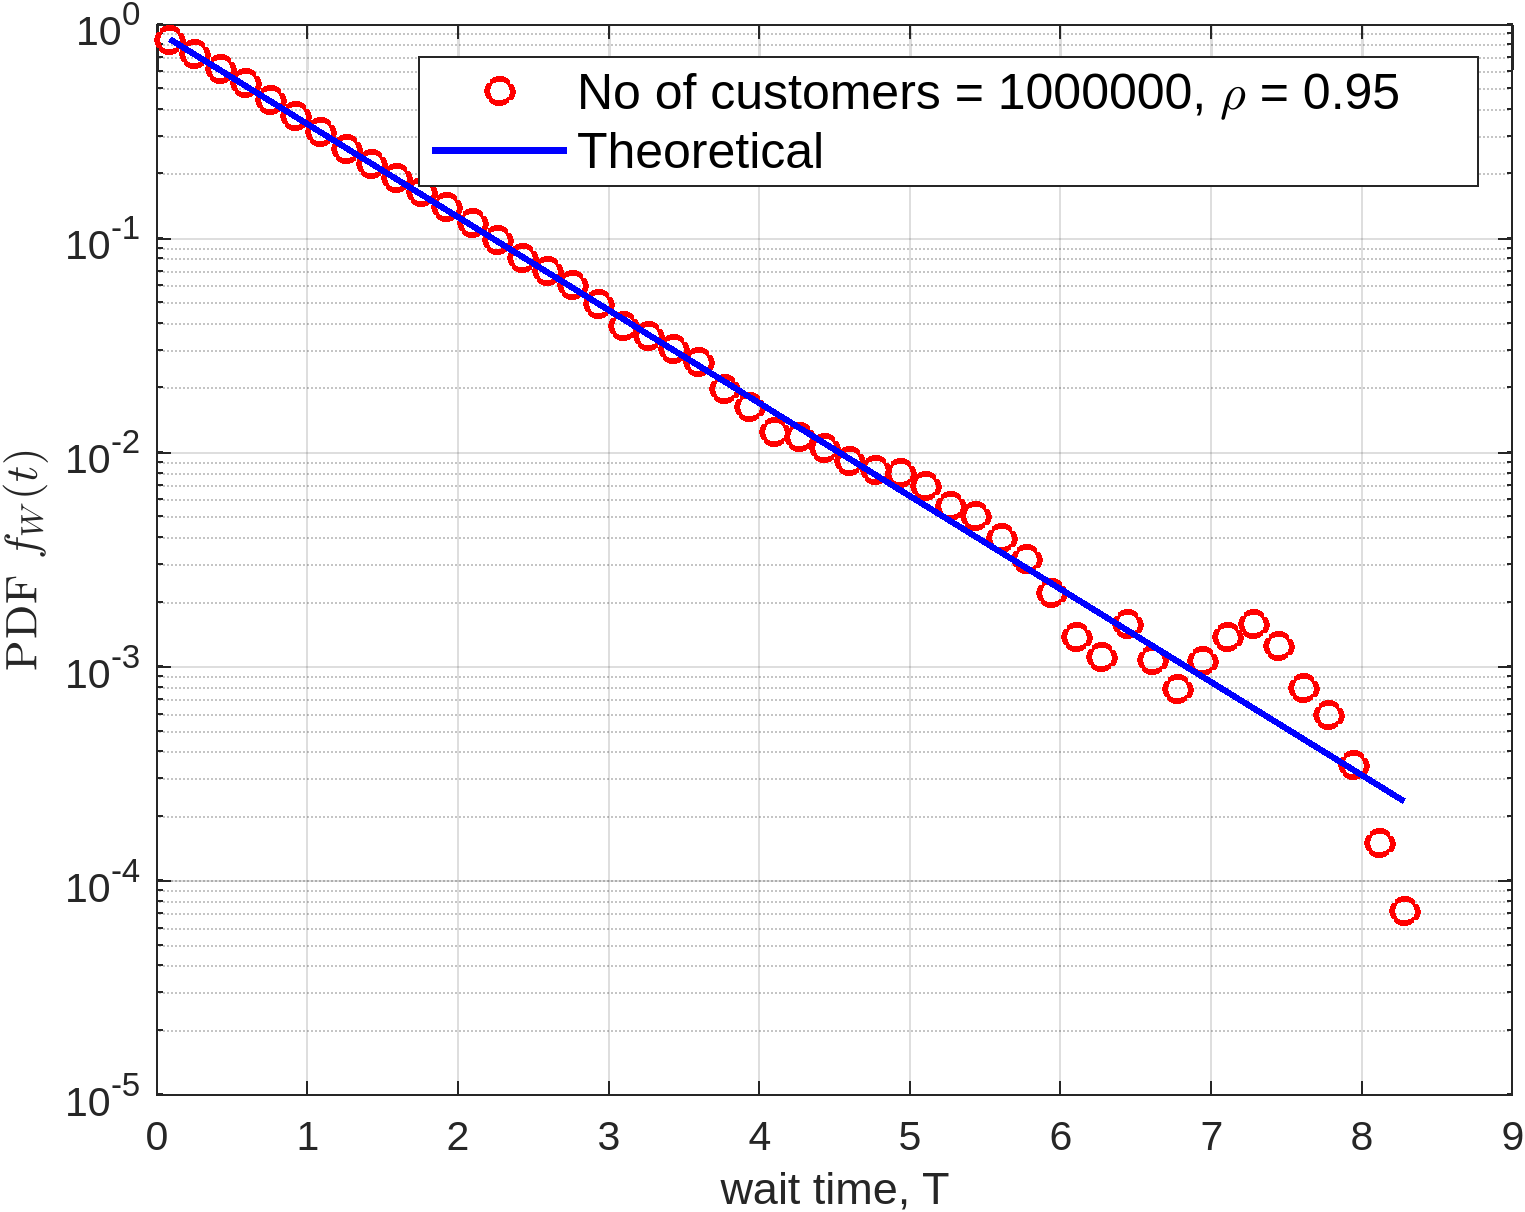
\includegraphics[width=200px]{../code/figures/waiting_time_dist/semilogy_plot_no_customers_1000000_rho_0.95.png}
  }
  \caption{PDF of the waiting time in the system for high $\rho$}  
  \label{PDF_W_high_more_cust}
\end{figure}

\subsection{PMF of $N(t)$}
\begin{figure}[H]
  \centering
  \subfloat[]{
    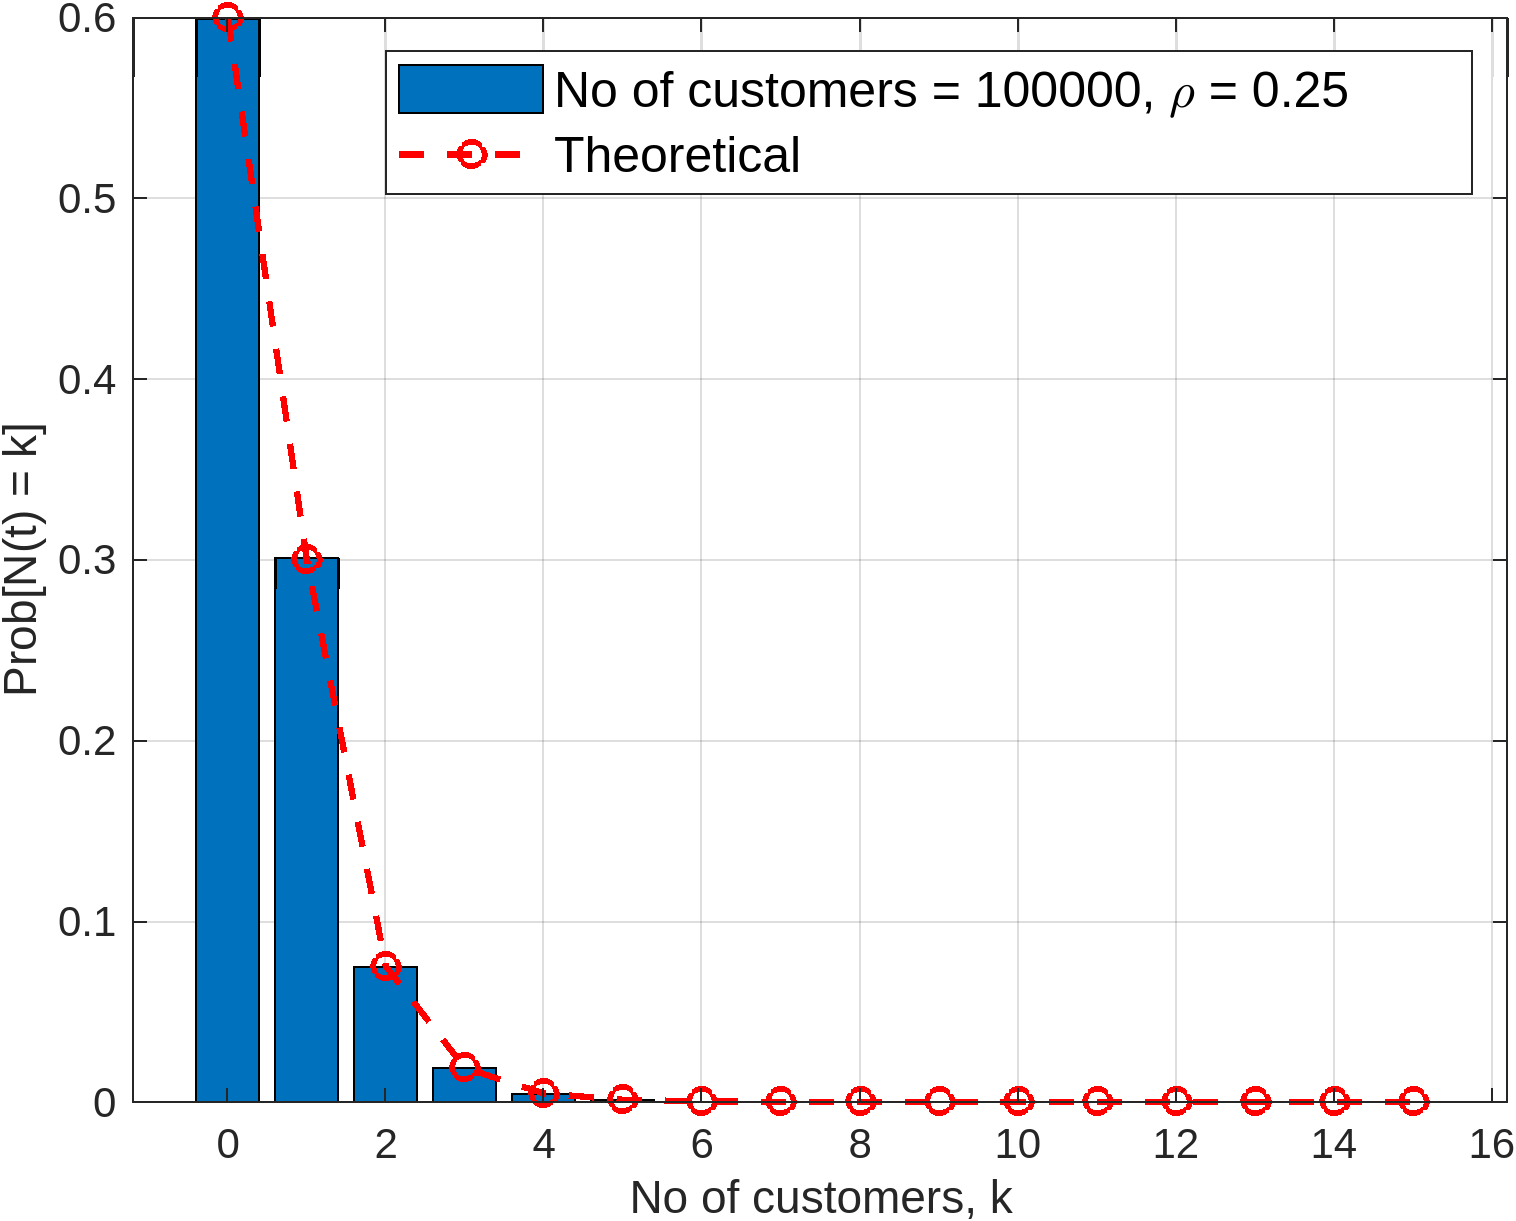
\includegraphics[width=200px]{../code/figures/N_PMF/semilogy_plot_no_customers_100000_rho_0.25.png}
  }
  \subfloat[]{
    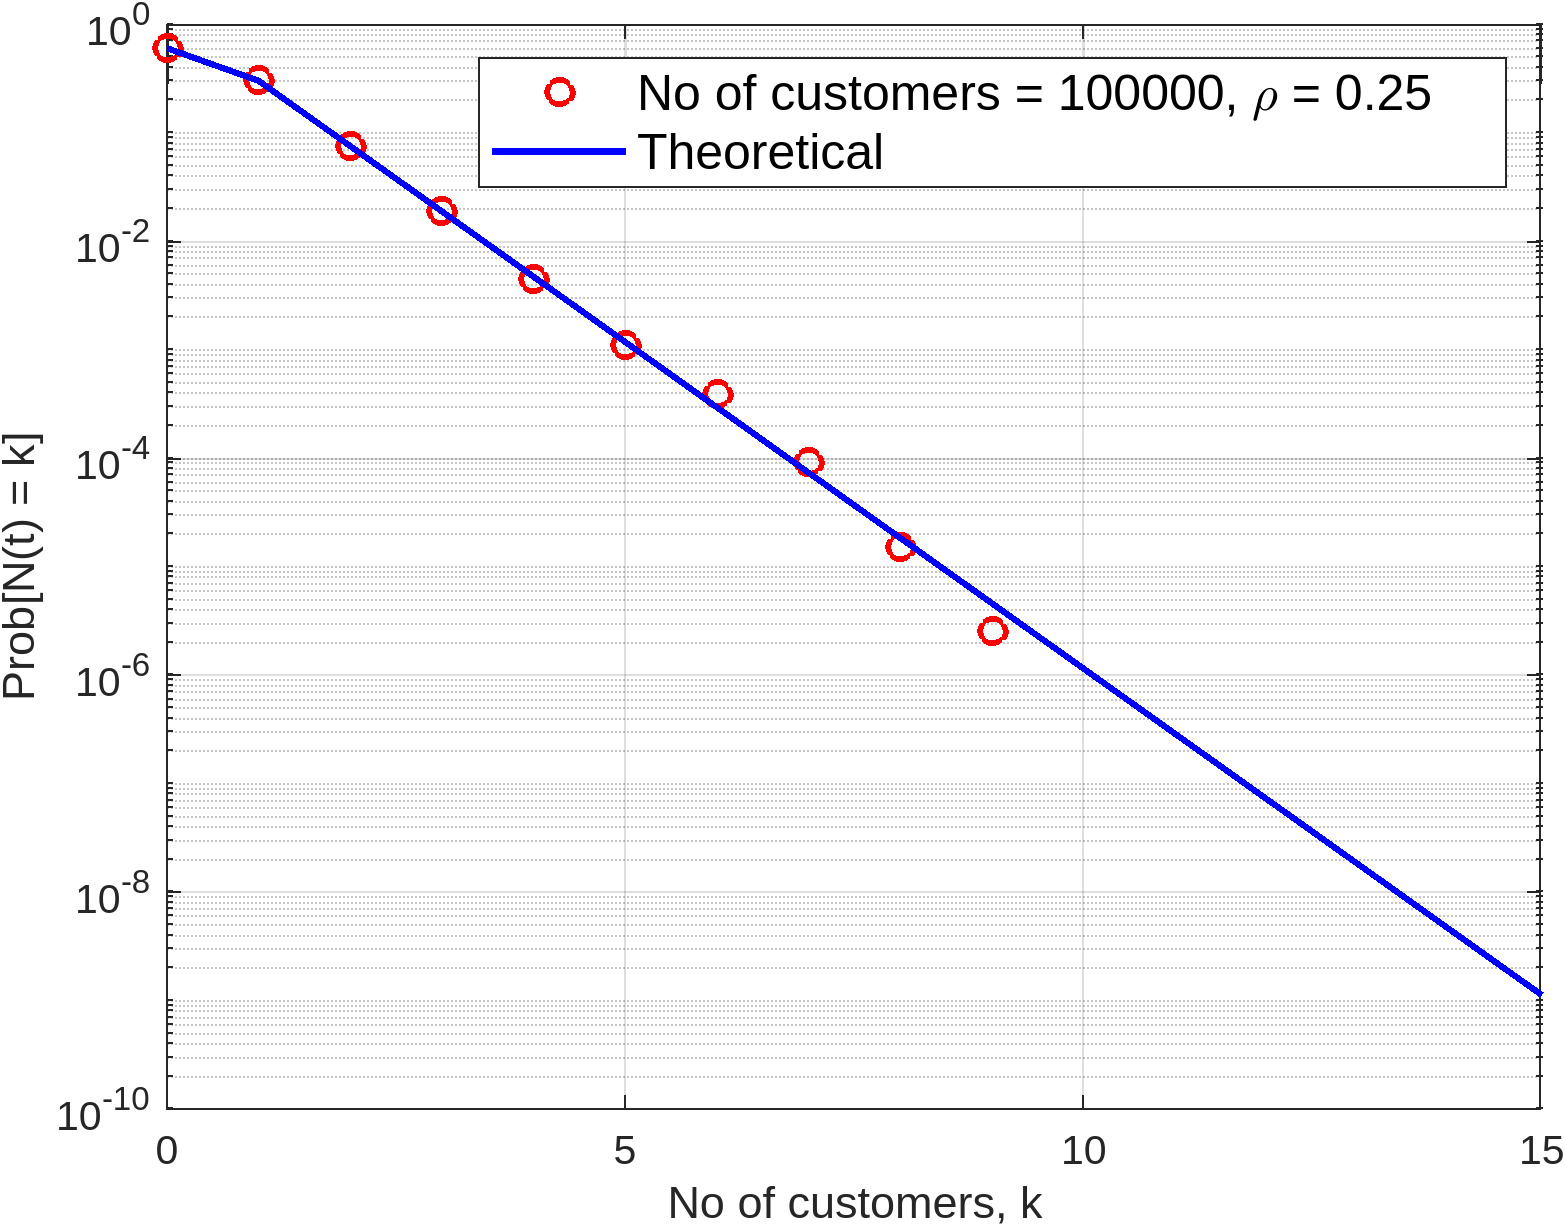
\includegraphics[width=200px]{../code/figures/N_PMF/bar_plot_no_customers_100000_rho_0.25.png}
  }
  \hspace{0px}
  \subfloat[]{
    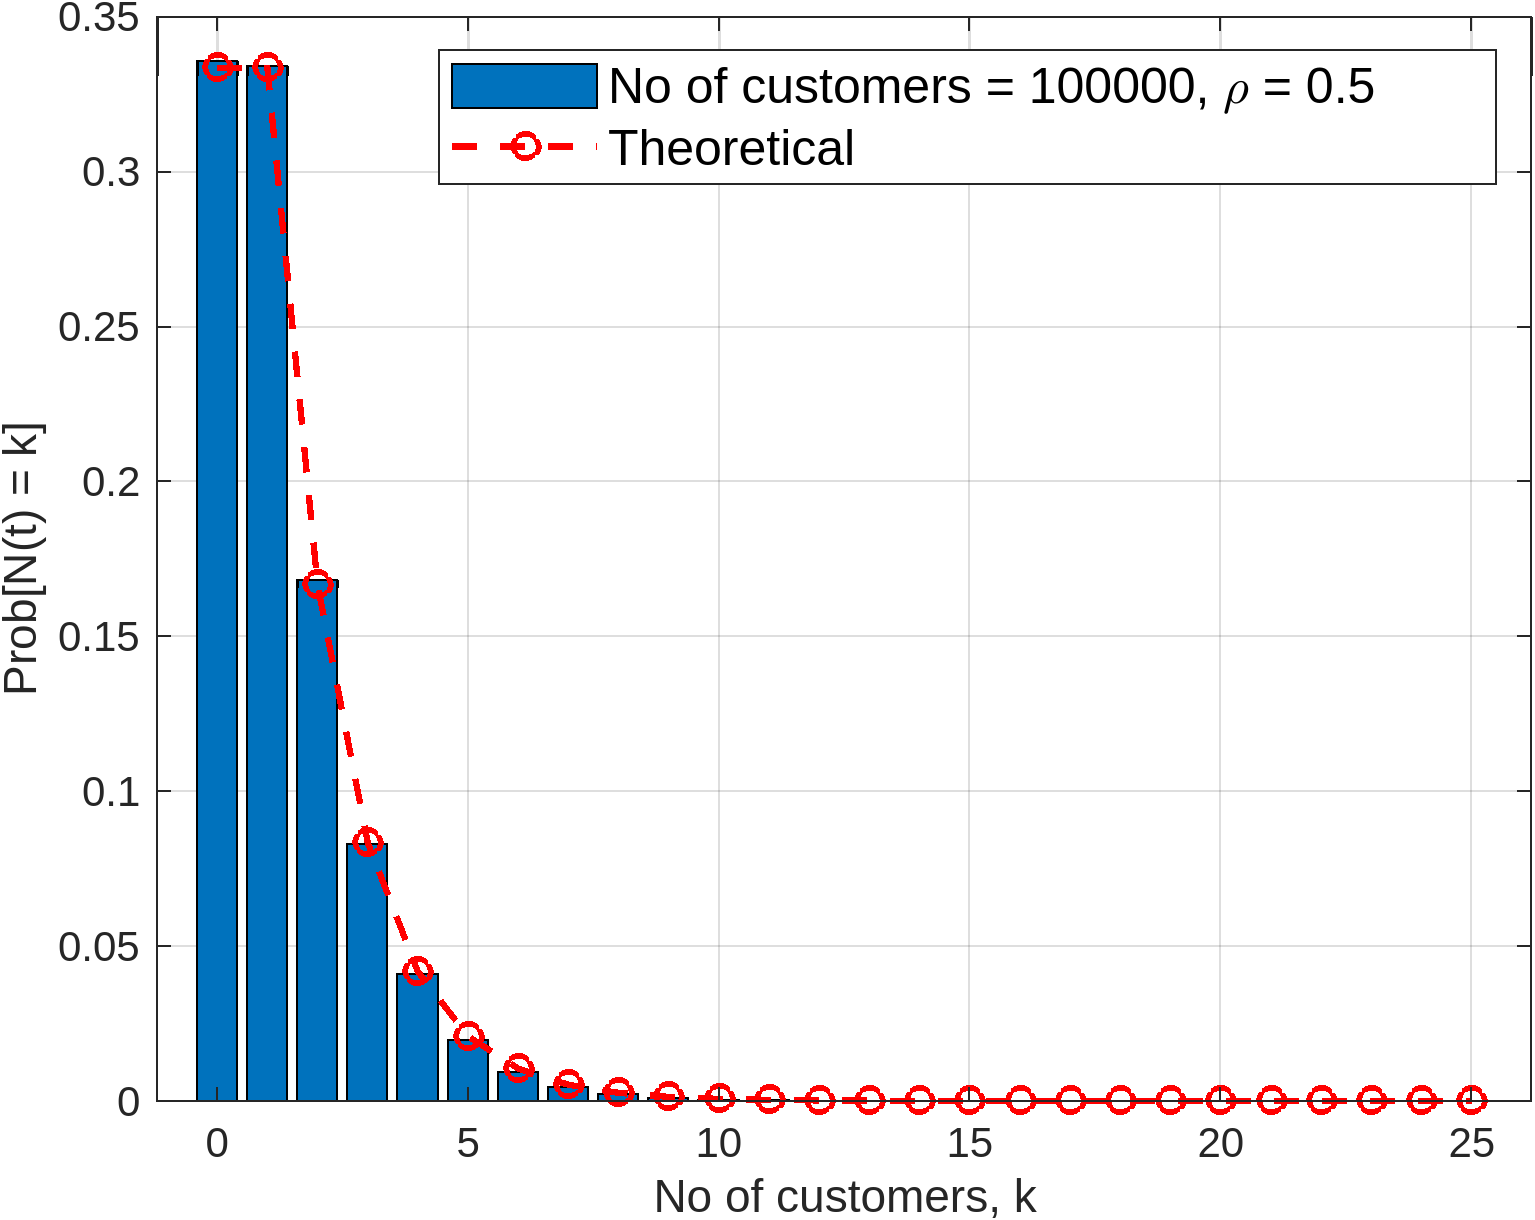
\includegraphics[width=200px]{../code/figures/N_PMF/semilogy_plot_no_customers_100000_rho_0.5.png}
  }
  \subfloat[]{
    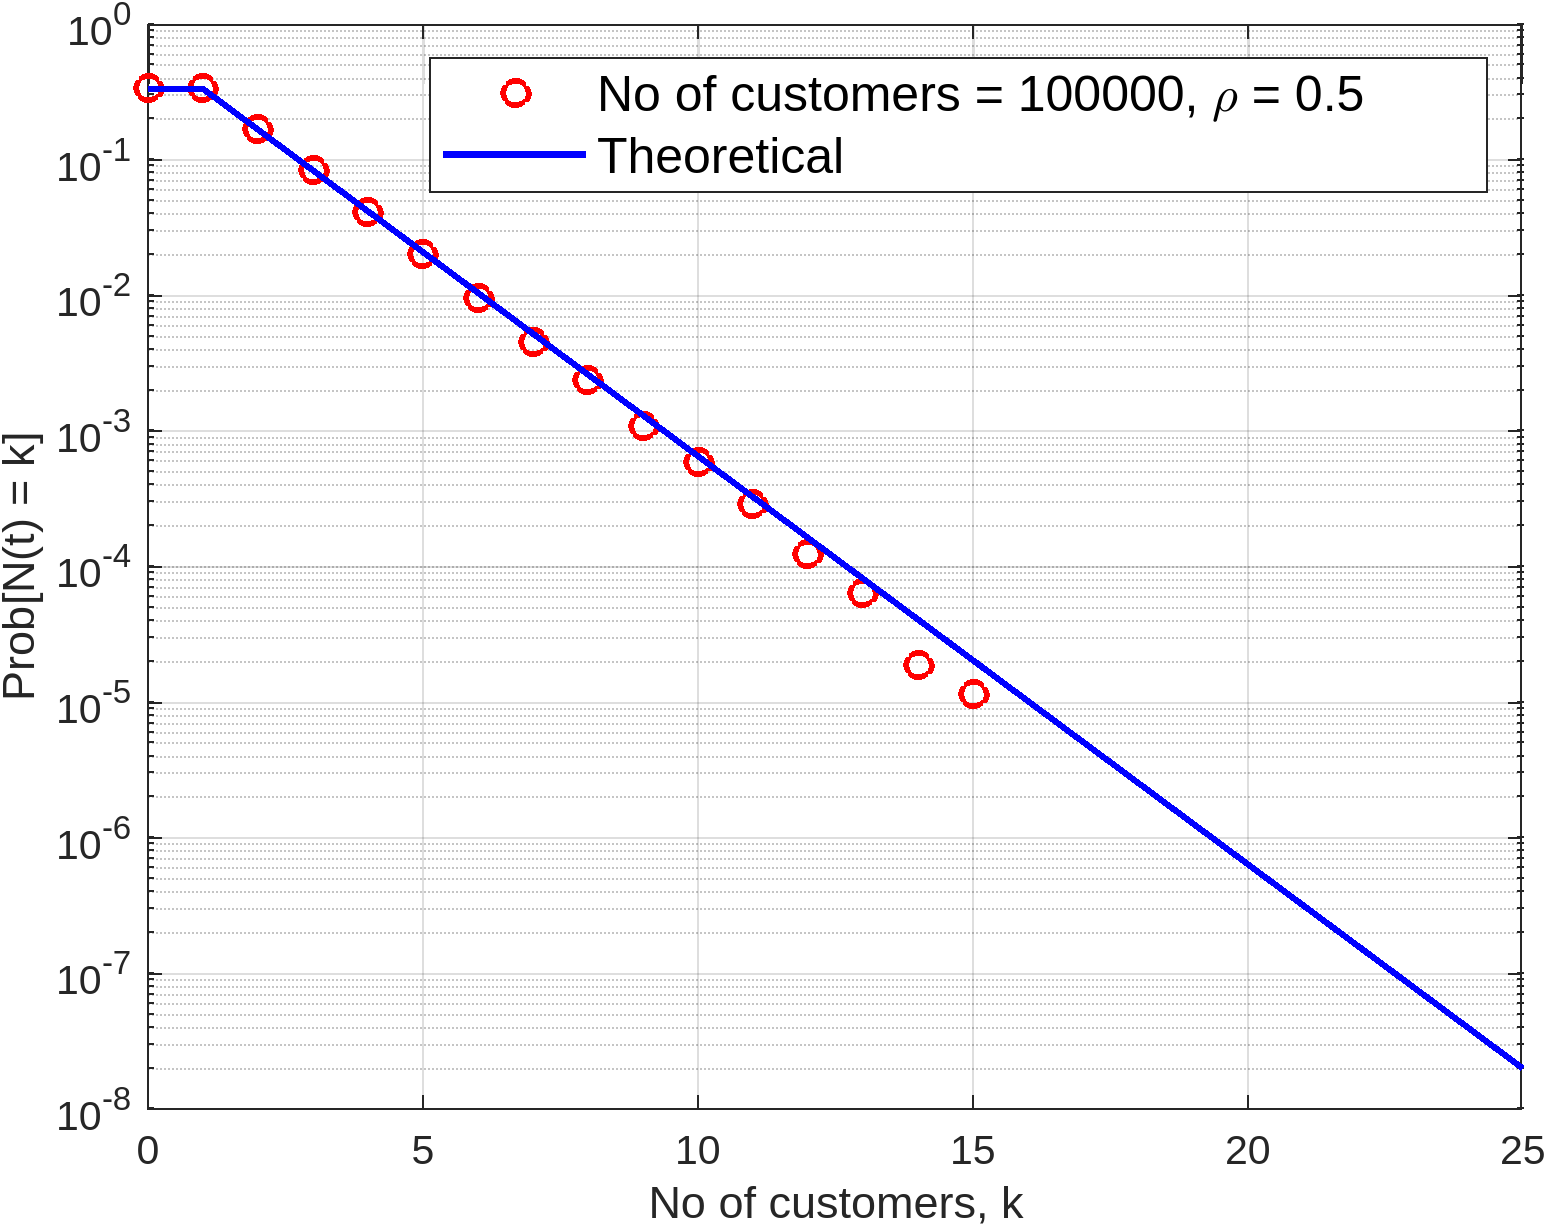
\includegraphics[width=200px]{../code/figures/N_PMF/bar_plot_no_customers_100000_rho_0.5.png}
  }
  \caption{PMF of $N(t)$  for low and medium traffic intensities}  
  \label{PMF_N_low_med}
\end{figure}

\begin{figure}[H]
  \centering
  \subfloat[]{
    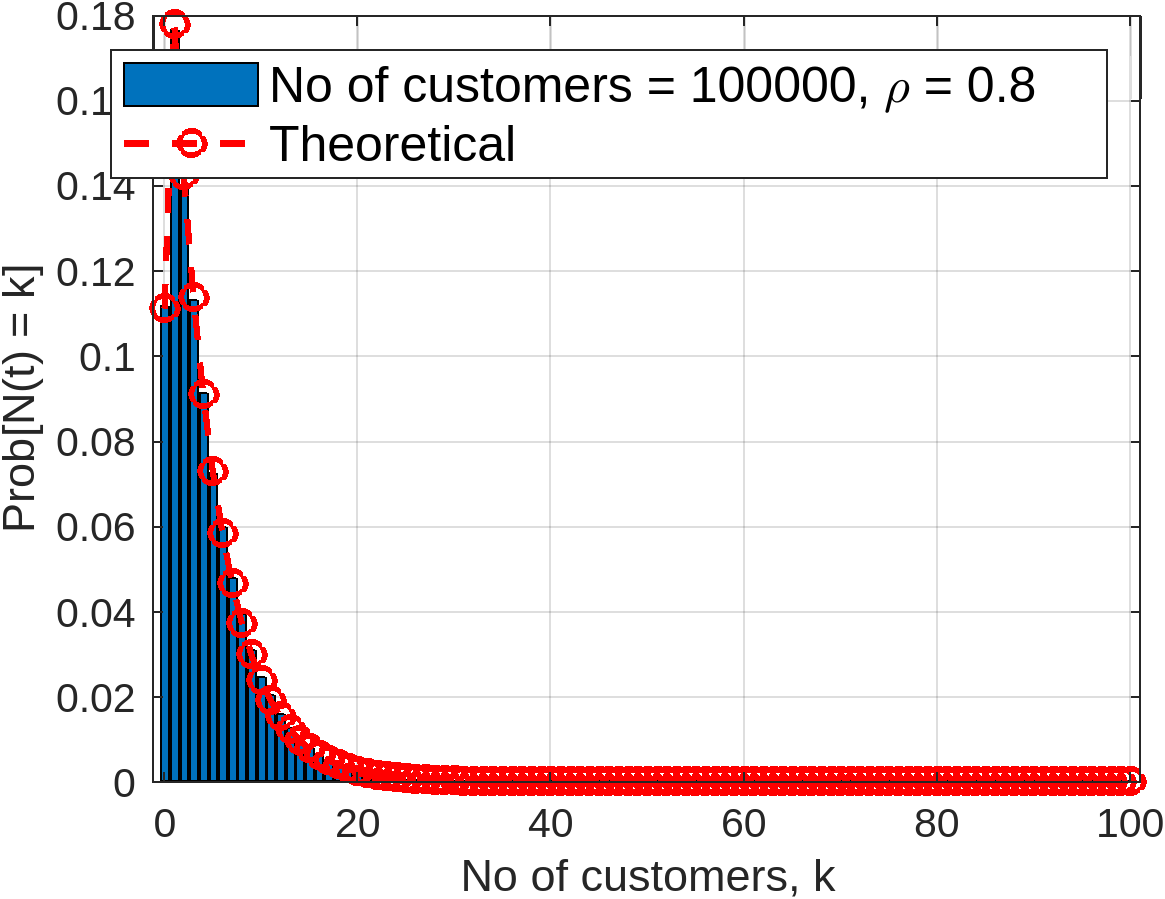
\includegraphics[width=200px]{../code/figures/N_PMF/semilogy_plot_no_customers_100000_rho_0.8.png}
  }
  \subfloat[]{
    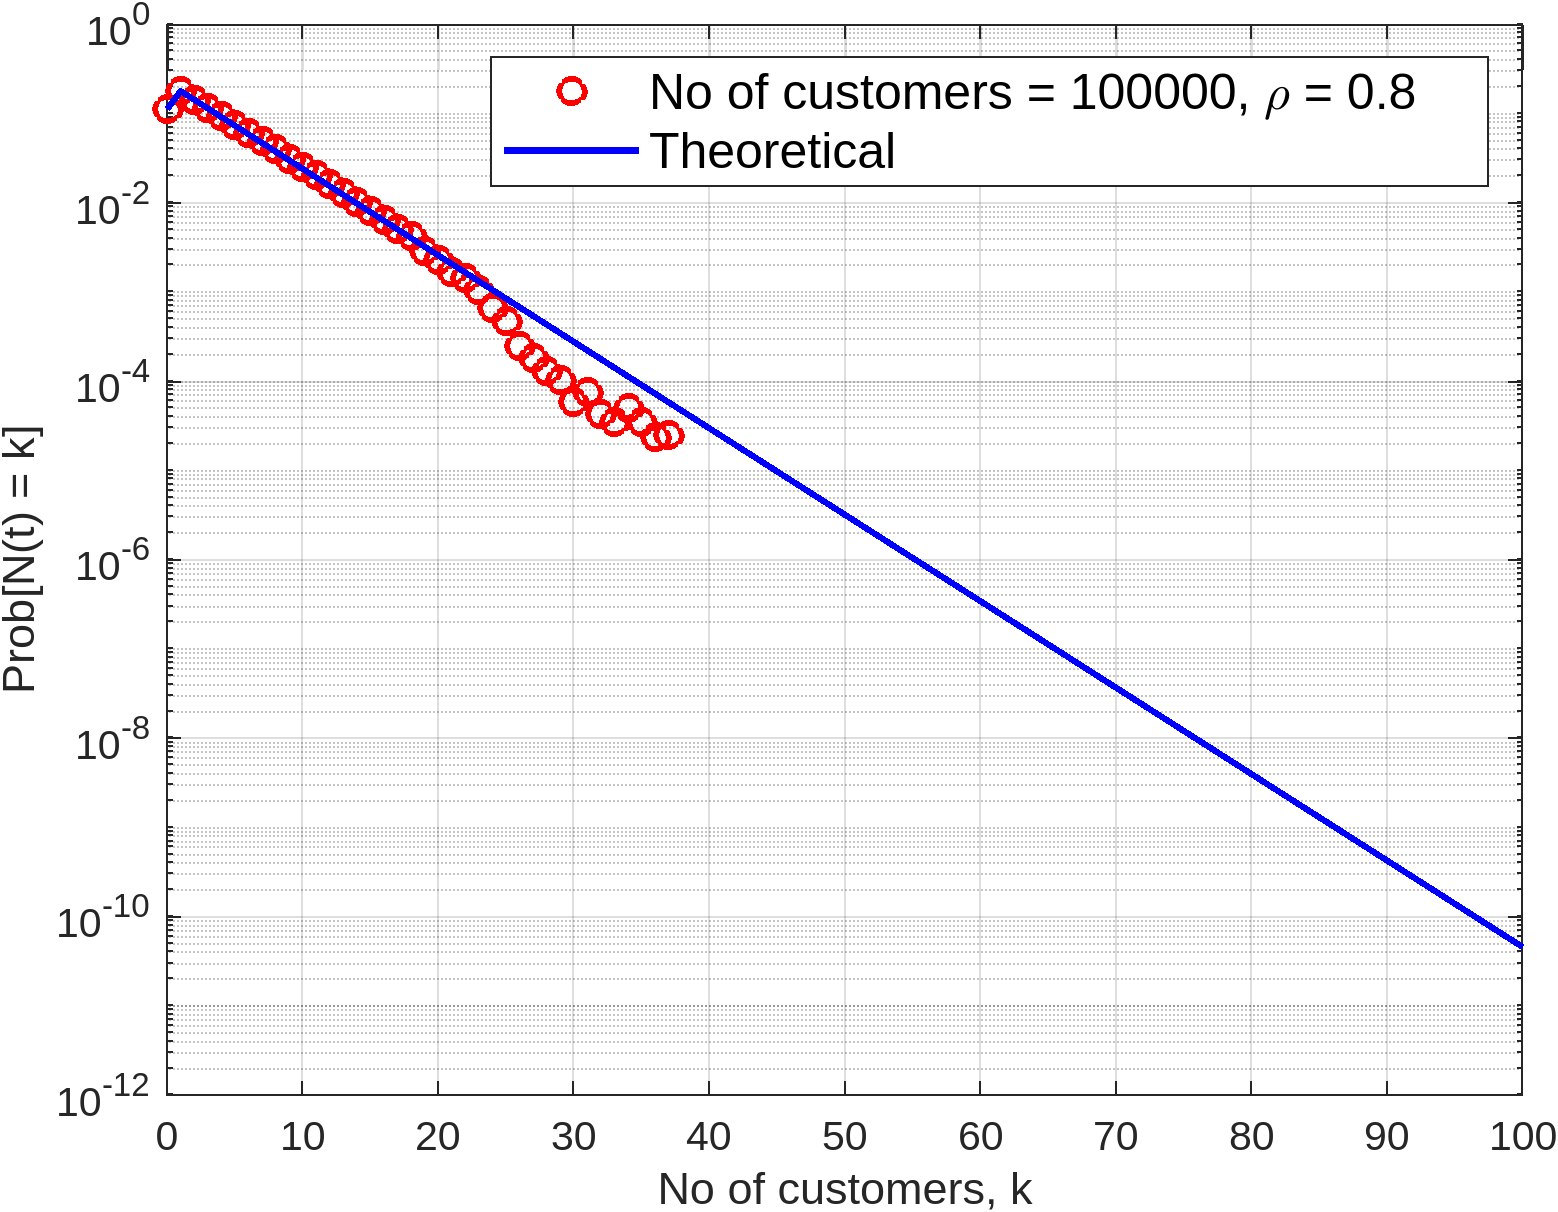
\includegraphics[width=200px]{../code/figures/N_PMF/bar_plot_no_customers_100000_rho_0.8.png}
  }
  \hspace{0px}
  \subfloat[]{
    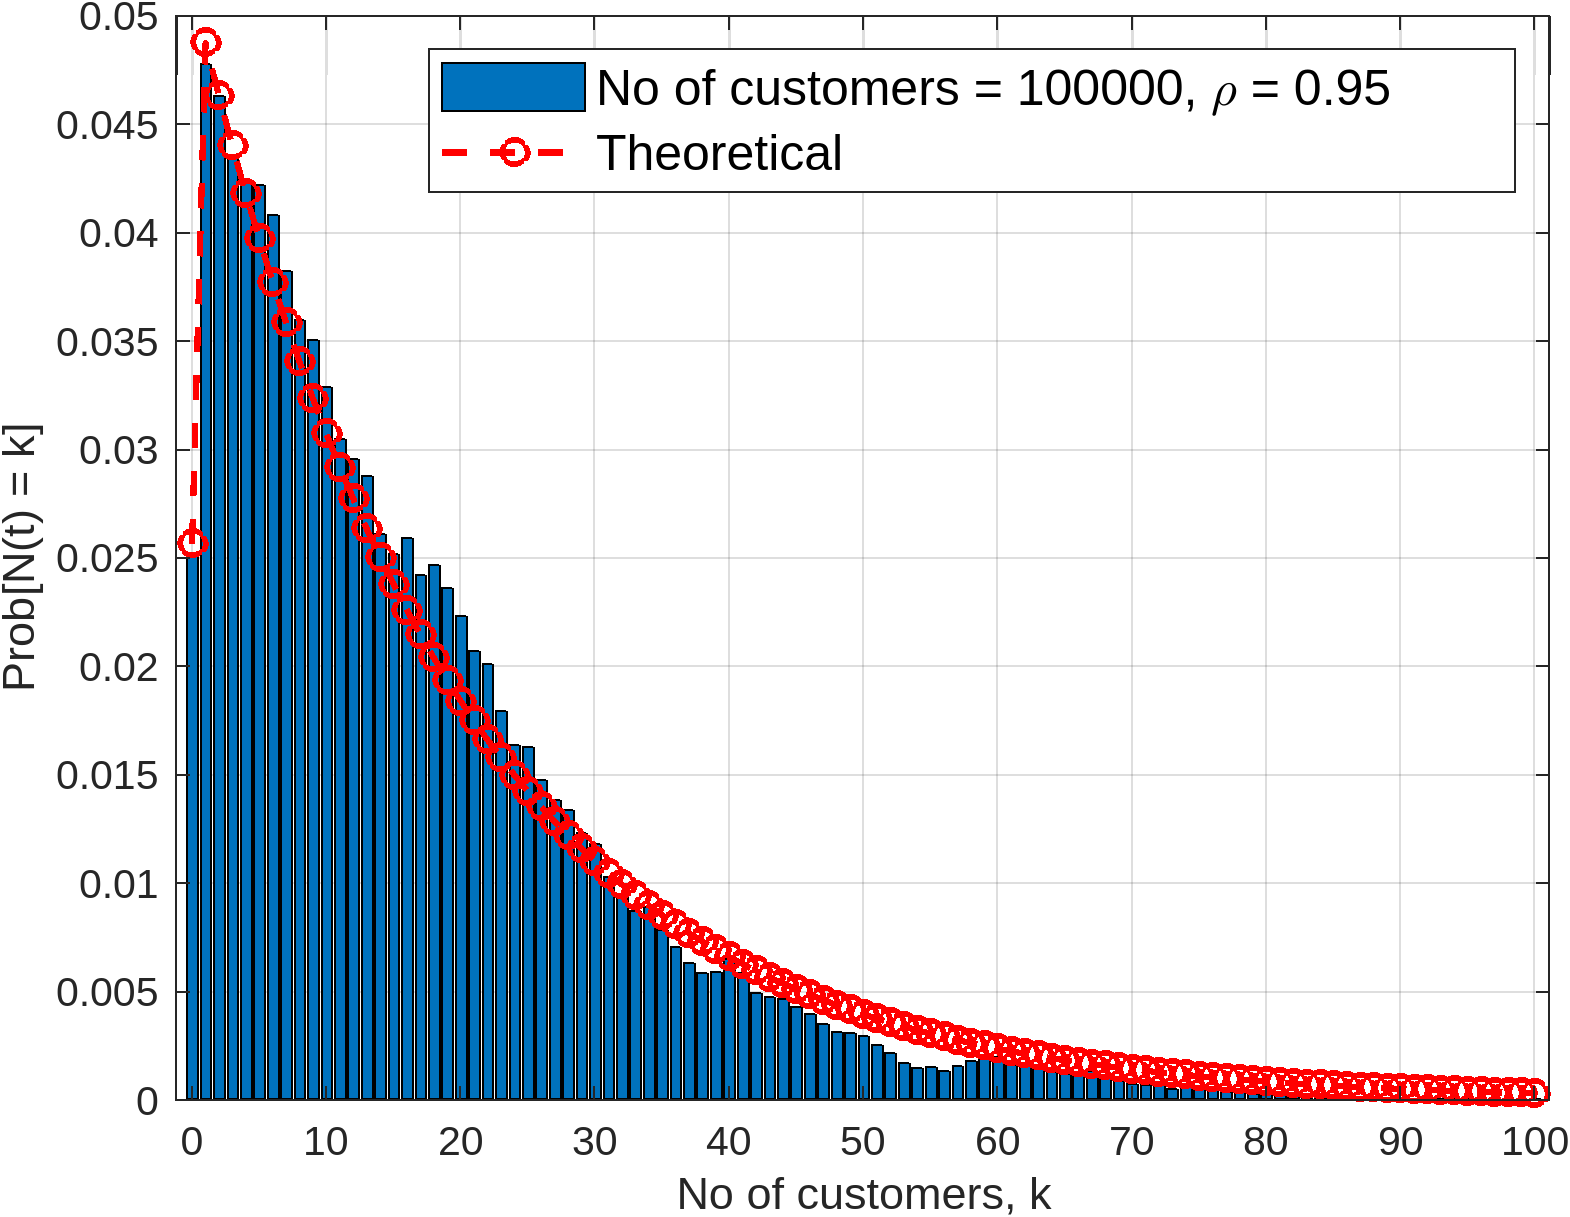
\includegraphics[width=200px]{../code/figures/N_PMF/semilogy_plot_no_customers_100000_rho_0.95.png}
  }
  \subfloat[]{
    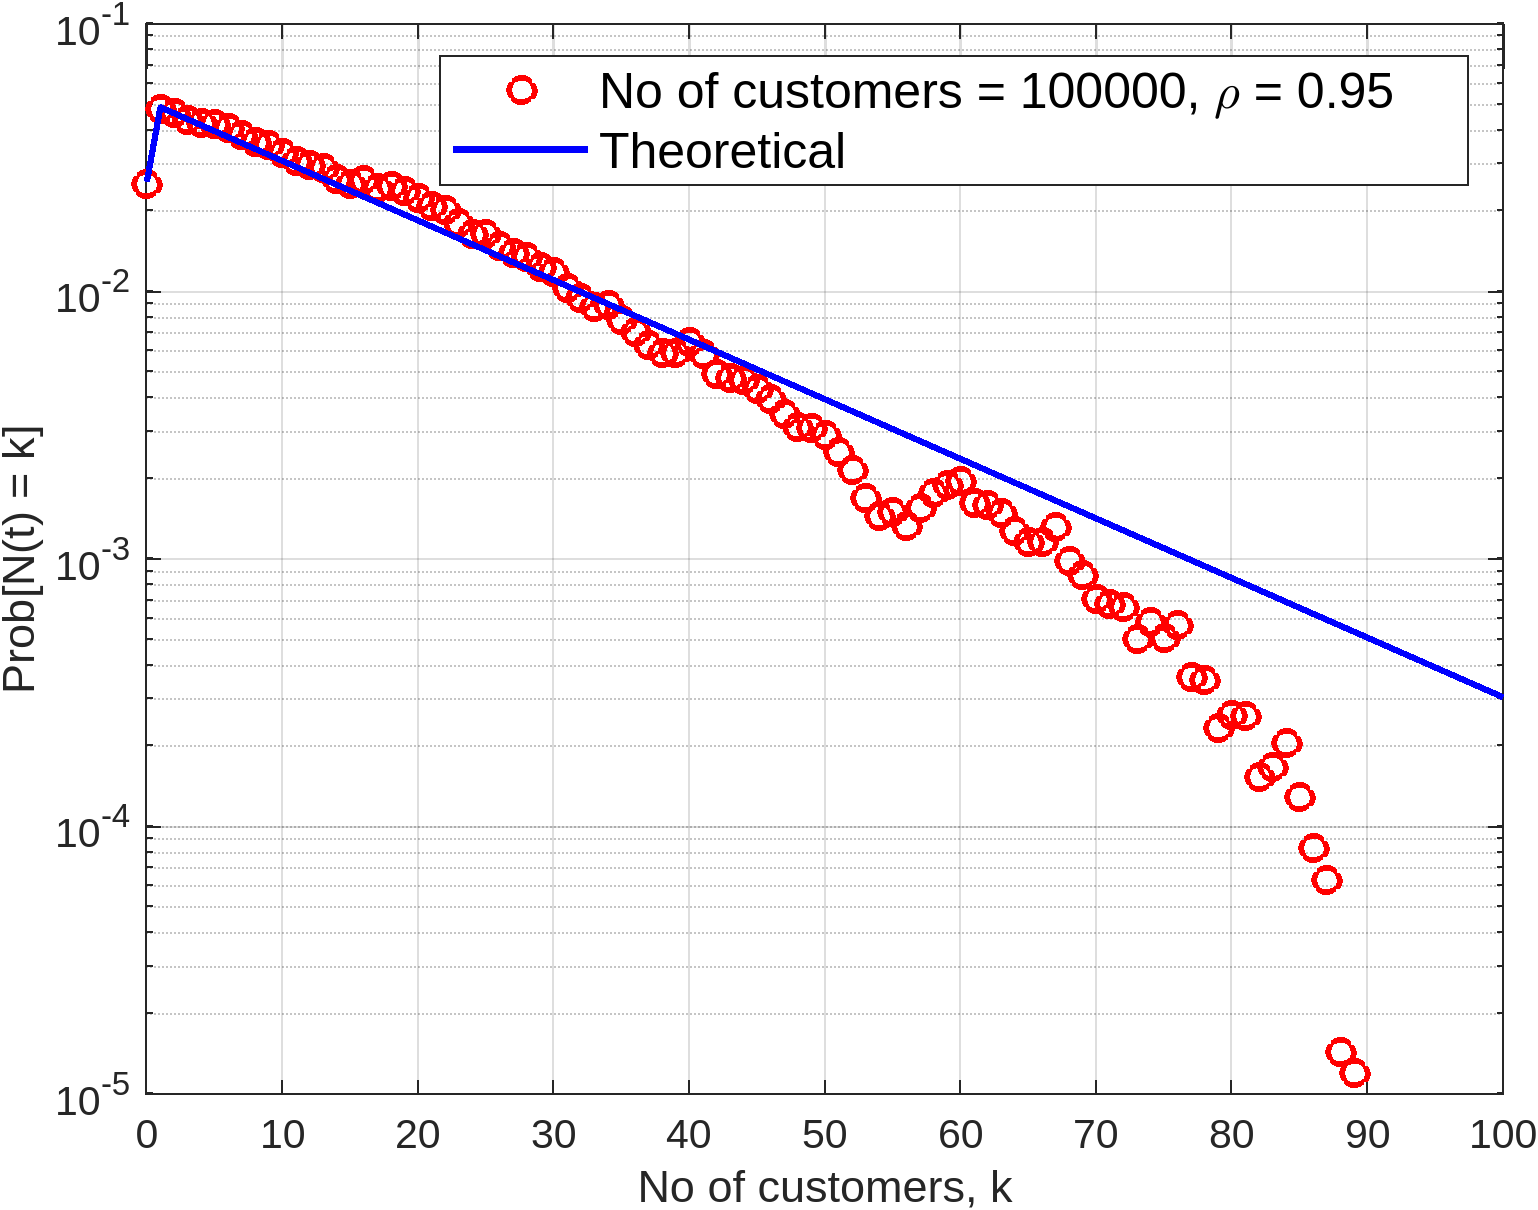
\includegraphics[width=200px]{../code/figures/N_PMF/bar_plot_no_customers_100000_rho_0.95.png}
  }
  \caption{PMF of $N(t)$  for high traffic intensity}  
  \label{PMF_N_high}
\end{figure}

Figure \ref{PMF_N_low_med} shows the probability mass function of the number of
customers in the system for low traffic intensity, $\rho = 0.25$ and medium traffic
intensity, $\rho=0.5$. We noticed that the probability of having 10 customers and more in the 
system for $\rho=0.25$ and the probability of having 15 customers or more in the system is 
almost zero (negligible). The theoretical and the empirical PMF are in an excellent agreement 
with one another. 

Figure \ref{PMF_N_high} show the PMF of $N(t)$ for high intensities, and we notice that the 
probability of having more customers has increased dramatically from the case of low 
and medium intensities. For $\rho=0.8$, the empirical distribution agrees well with the theoretical
one, but the one for $\rho=0.95$ deviates from the theoretical distribution, especially for higher 
states. To improve the results, we have increased the number of customers to 1000000.
The results for the increment is displayed in Figure \ref{PMF_N_high_more_cust}.

\begin{figure}[H]
  \centering
  \subfloat[]{
    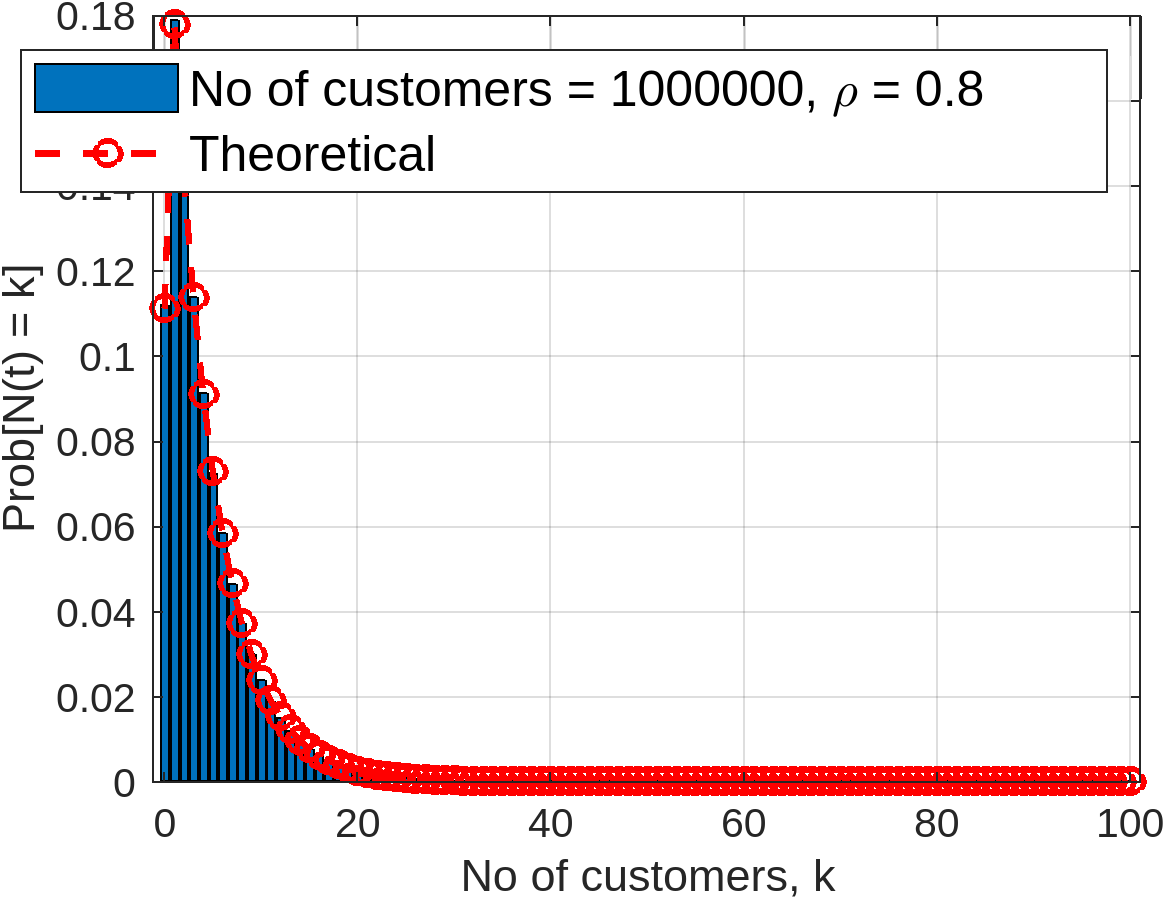
\includegraphics[width=200px]{../code/figures/N_PMF/semilogy_plot_no_customers_1000000_rho_0.8.png}
  }
  \subfloat[]{
    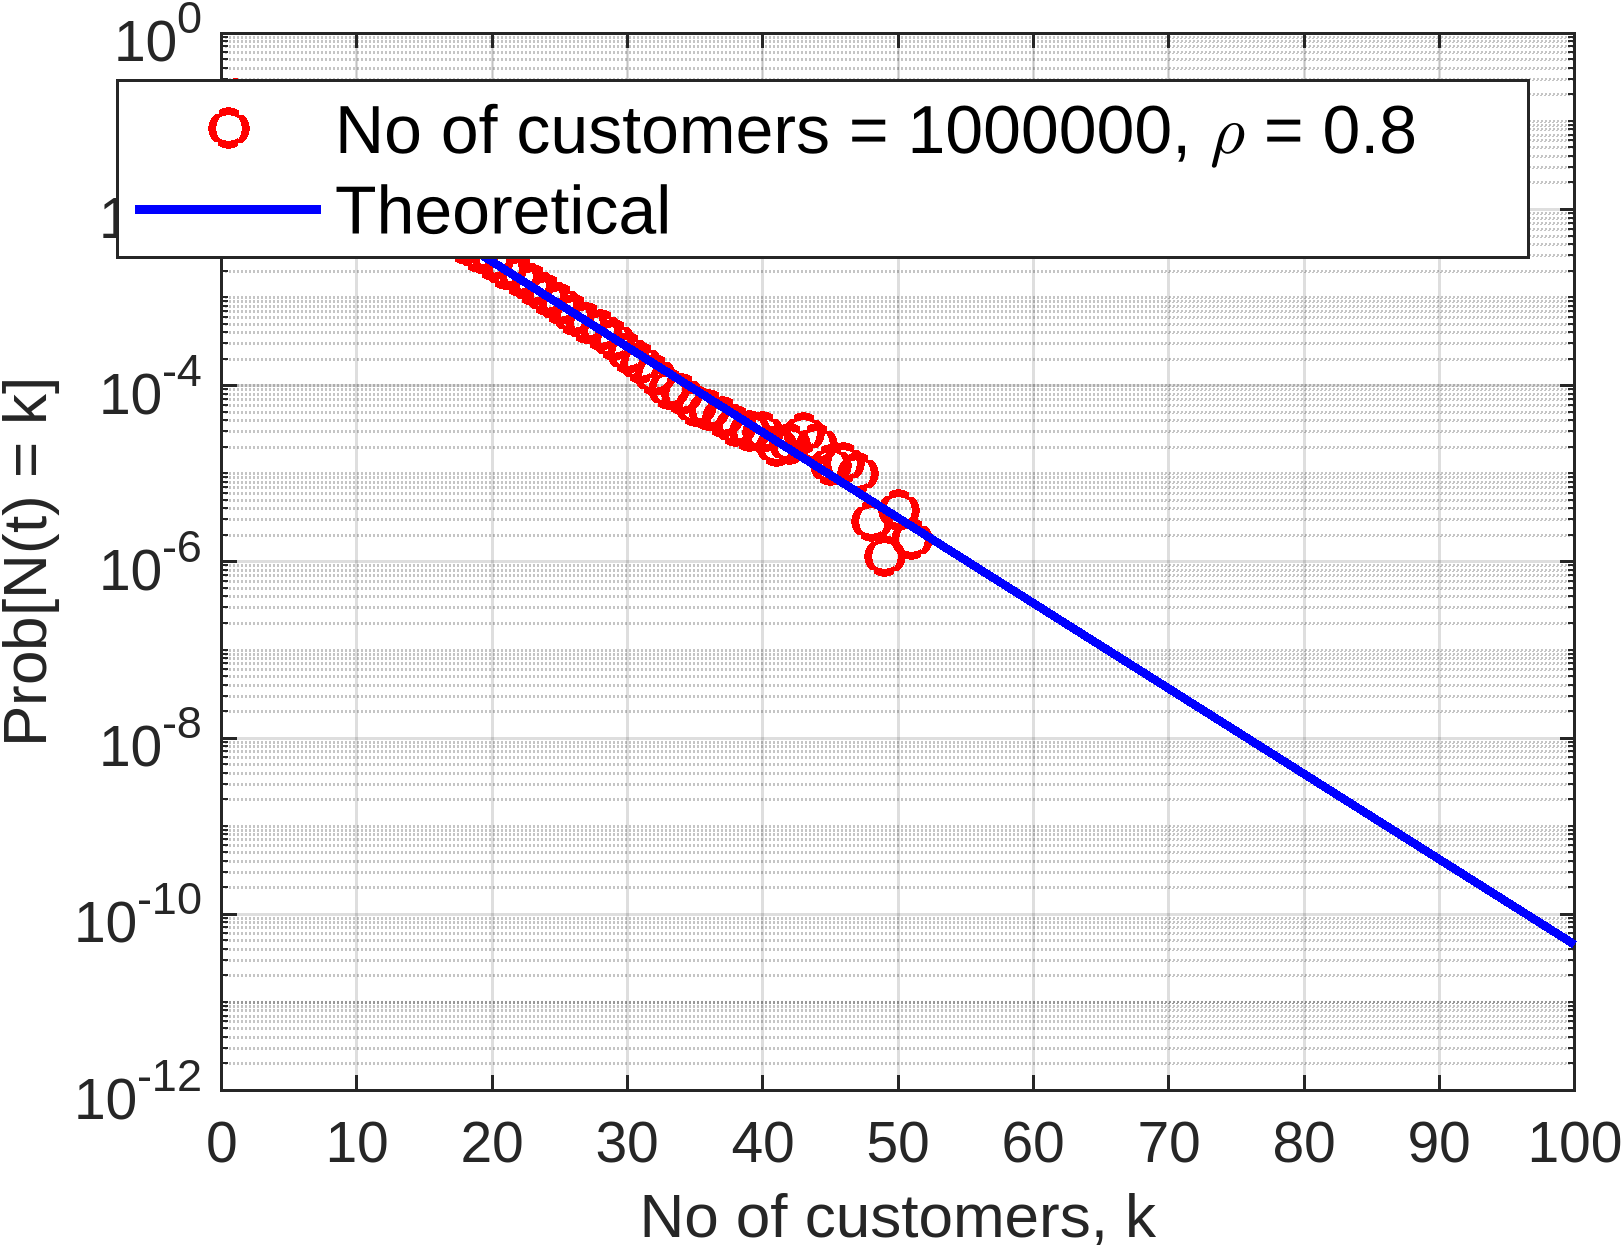
\includegraphics[width=200px]{../code/figures/N_PMF/bar_plot_no_customers_1000000_rho_0.8.png}
  }
  \hspace{0px}
  \subfloat[]{
    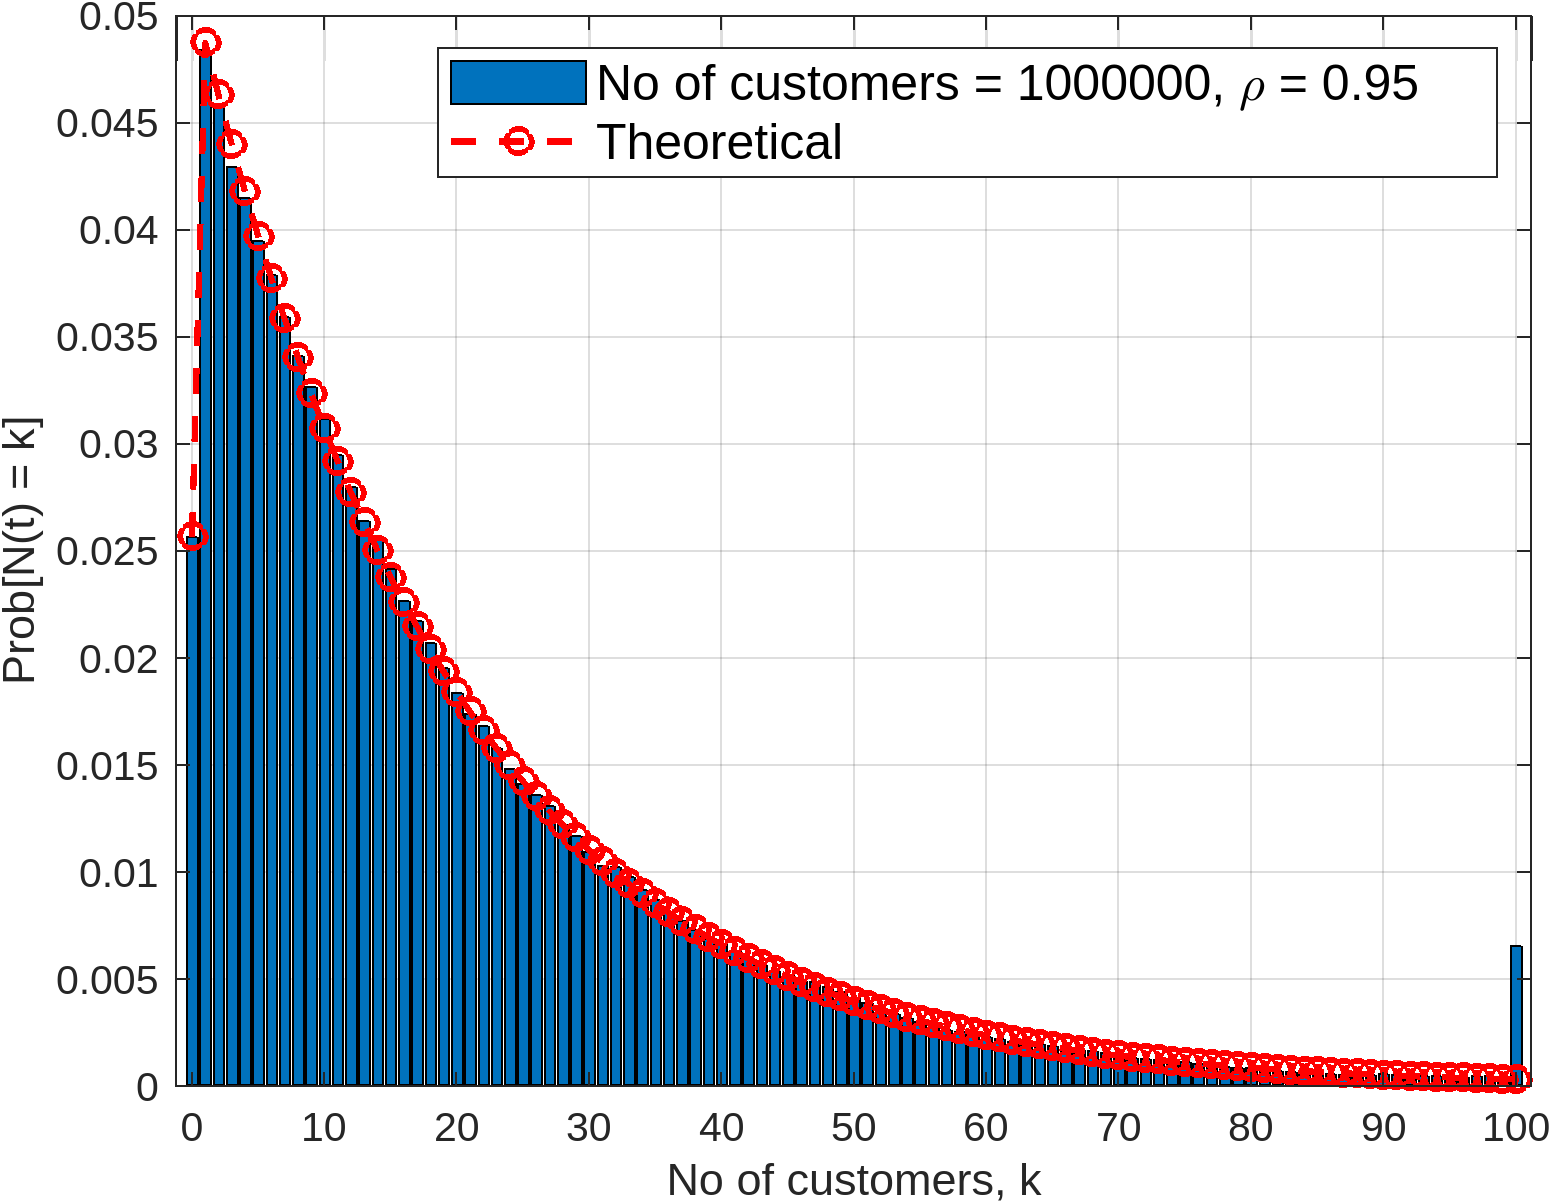
\includegraphics[width=200px]{../code/figures/N_PMF/semilogy_plot_no_customers_1000000_rho_0.95.png}
  }
  \subfloat[]{
    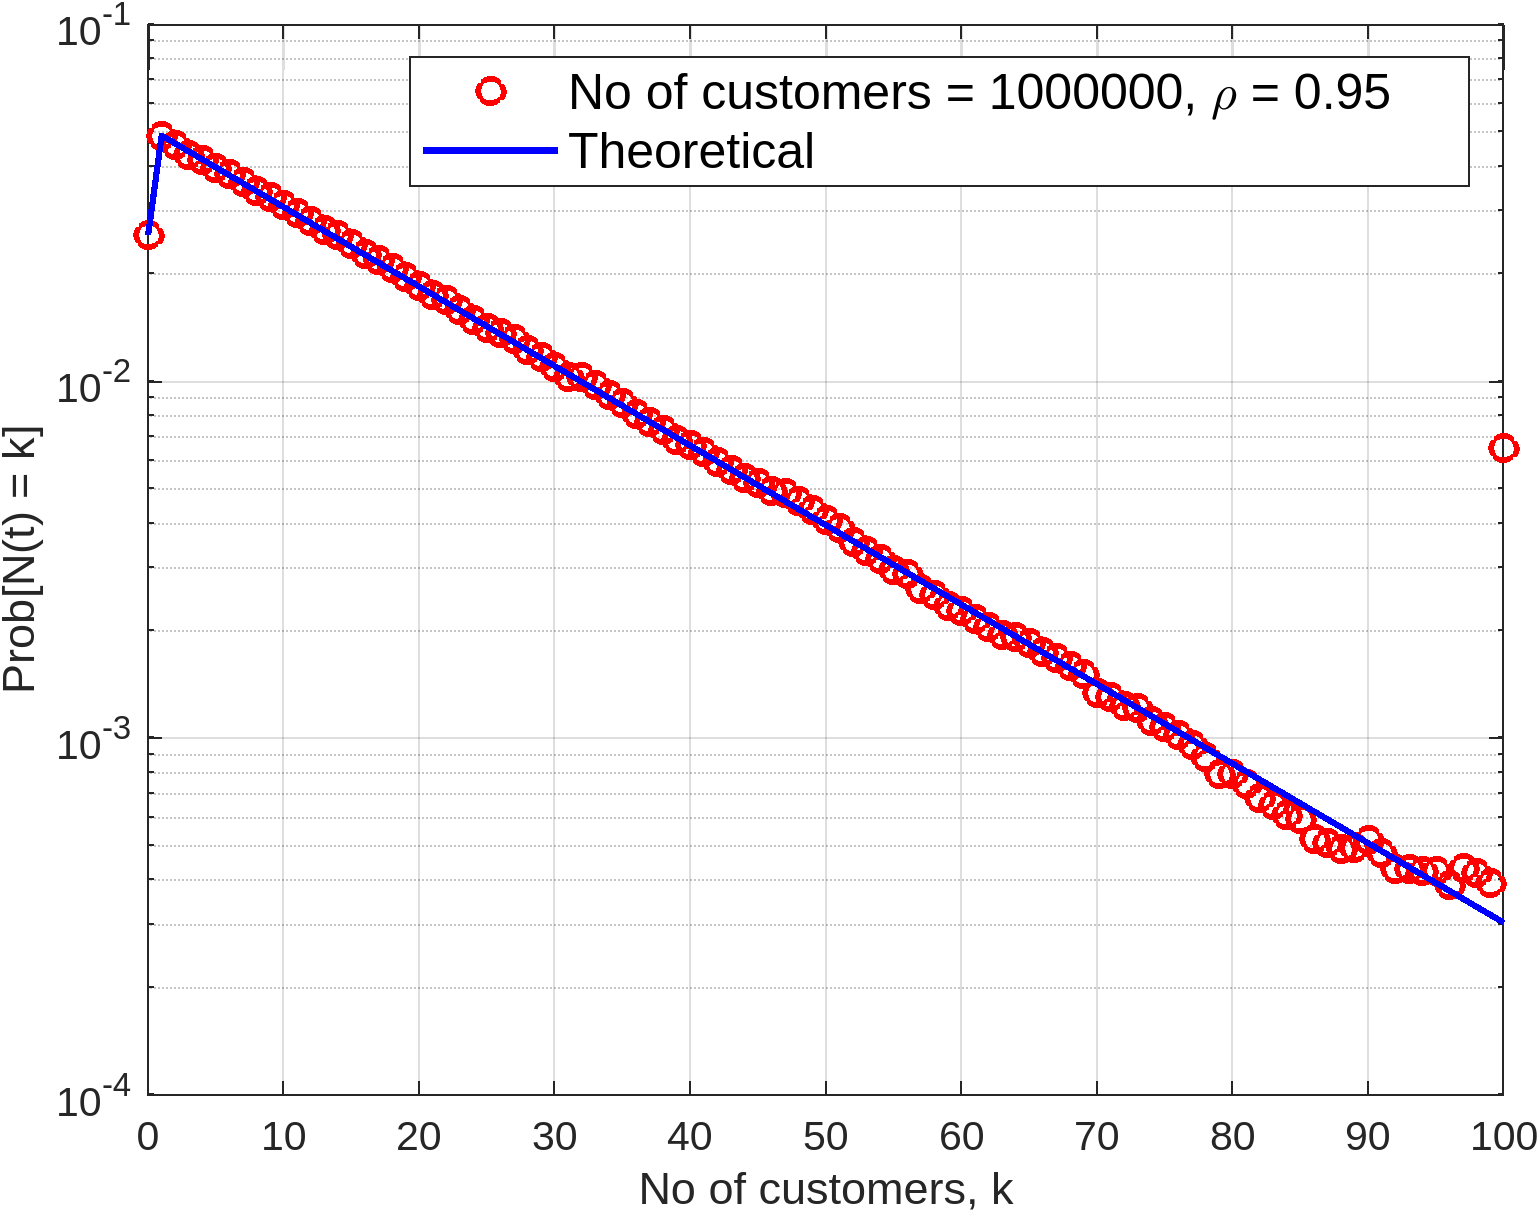
\includegraphics[width=200px]{../code/figures/N_PMF/bar_plot_no_customers_1000000_rho_0.95.png}
  }
  \caption{PMF of $N(t)$  for high traffic intensity and 1000000 customers}  
  \label{PMF_N_high_more_cust}
\end{figure}

\subsection{Prob$[W > 0]$ vs $c$}
\begin{figure}
  \centering 
  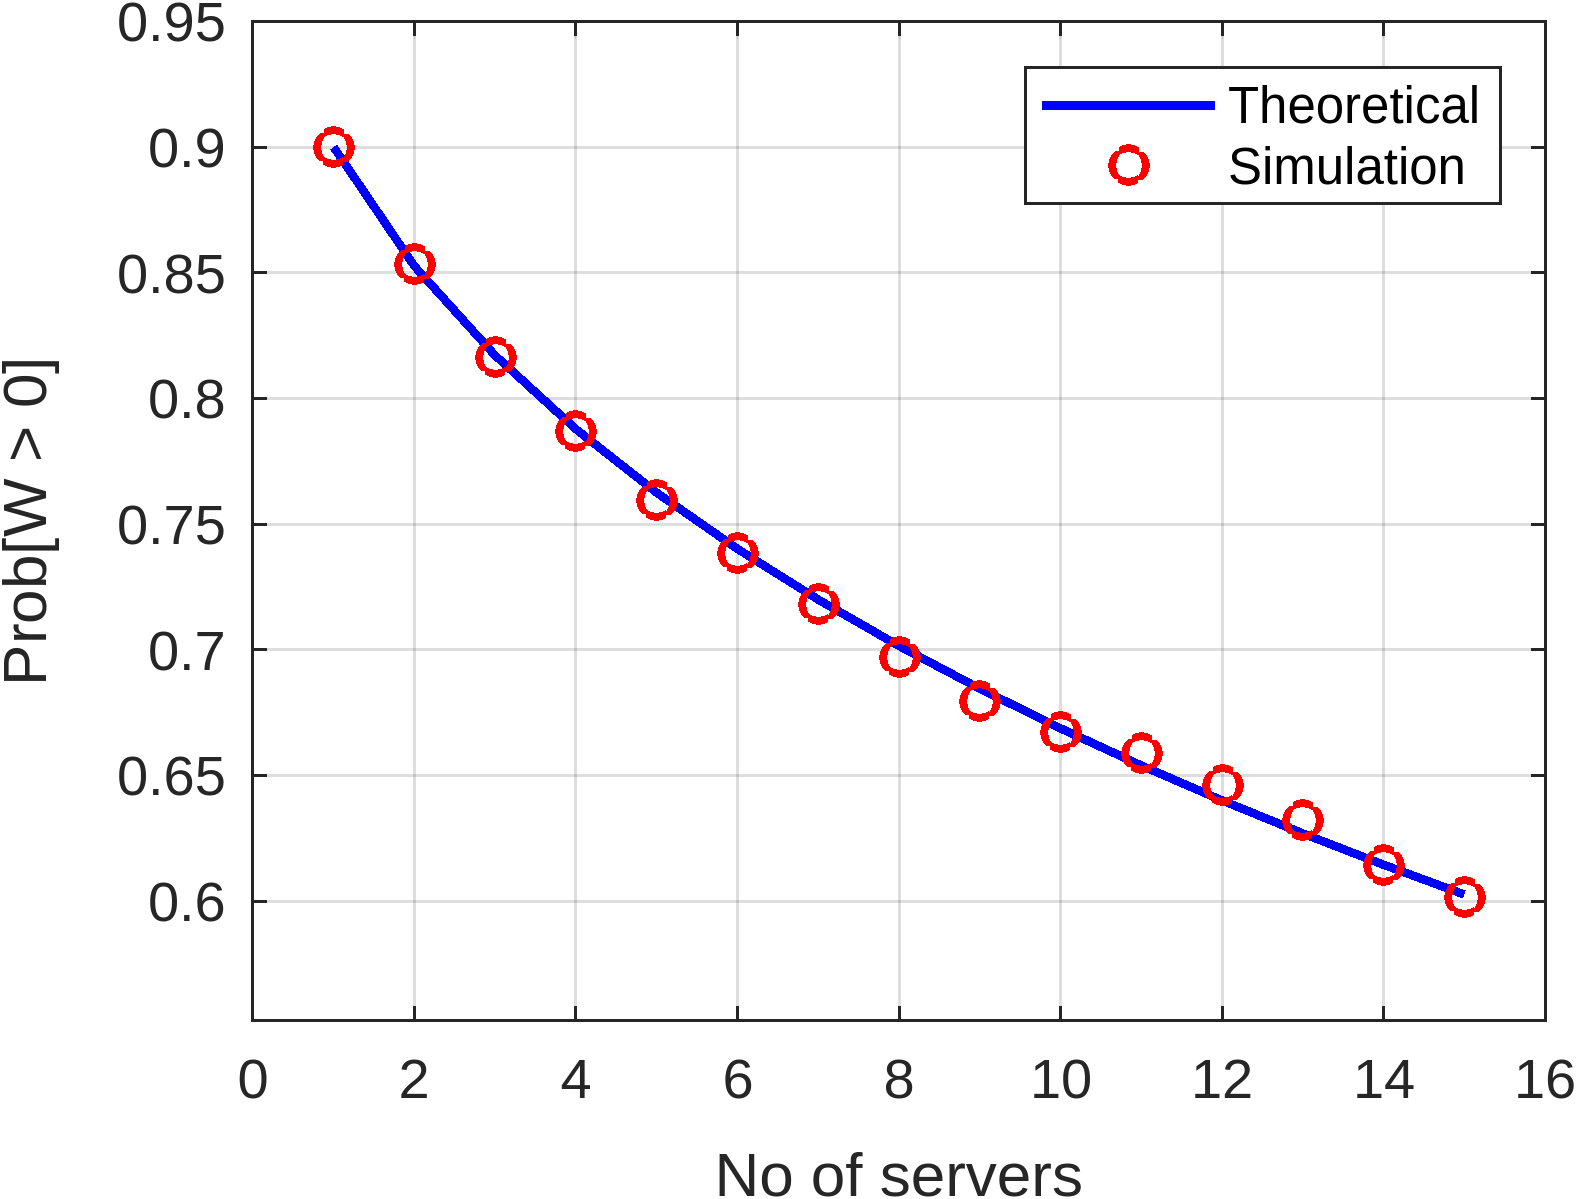
\includegraphics[width=250px]{../code/figures/pWaiting_vs_c/no_customers_1000000_max_c_15.png}
  \caption{Prob$[W > 0]$ vs $c$ for $\rho=0.9$}
  \label{W_vs_c}
\end{figure}

Figure \ref{W_vs_c} shows the probability having to wait as function of the number of servers 
in the system for a fixed traffic intensity. The plot indicates that probability of having to 
wait decreases as the number of the servers increase, which is intuitive since more servers means 
more total service rate and hence less waiting time and thus the probability of having to wait decreases. Furthermore, the 
empirical curve agrees with theoretical one.

\section{Conclusion}
We have simulated M/M/c queueing system with an infinite buffer, and we 
have obtained the PDFs for the total time and the waiting time and the PMF 
for the number of customers in the system. Furthermore, the averages of the 
total time spent in the system, the waiting time in the queue, the number 
of customers in the system, and the number of customers in the queue were 
acquired through simulation. Additionally, the probability of having to wait 
for different number of servers were studied, and we observed that the probability
of waiting decreases as the number of servers increases as expected.
The simulation output shows an excellent agreement
with the theoretical formulas, which indicates that the used code is able to 
simulate the system properly. 


\newpage
\section*{Appendix}
\begin{lstlisting}[style=Matlab-editor, basicstyle=\ttfamily\footnotesize]
    function [DT, startList, serviceTime] = simulation_loop(AT, ST, c)
      numCustomers = length(AT);
      startList = zeros(1, numCustomers);
      DT = zeros(1, numCustomers);
      serverList = zeros(1, c); % Initialize server list with c free servers
      serverID = zeros(1, numCustomers);
      serviceTime = zeros(1, c);
      % Run simulation
      for i = 1:numCustomers
          % Find the earliest available server
          [~, idx] = min(serverList);
          earliestAvailableTime = serverList(idx);
          serverID(i) = idx;
          
          % Calculate the start time for the customer
          startTime = max(AT(i), earliestAvailableTime);
          startList(i) = startTime;
          
          % Calculate the departure time
          departureTime = startTime + ST(i);
          DT(i) = departureTime;
          
          % Update the server list
          serverList(idx) = departureTime;
          serviceTime(idx) = serviceTime(idx) + ST(i); 
      end
  end
  %---------------End od the function--------
  \end{lstlisting}
  
  \begin{lstlisting}[style=Matlab-editor, basicstyle=\ttfamily\footnotesize]
    %----------E[N], E[Nq], and PMF of N(t)-------------
    function [areaN, areaNq, simPMF] = PMF_and_track_N(AT, DT, c, N_max)
      N = 0; simPMF = zeros(1, N_max+1);
      areaN = 0; areaNq = 0;
      preEventTime = 0; clock = 0;
      i = 1; j = 1;
      sortedDT = sort(DT);
      while clock < max(AT)
          if AT(i) < sortedDT(j)
              clock = AT(i);
              timeInterval = clock - preEventTime;
              simPMF(min(N, N_max)+1) = simPMF(min(N, N_max)+1) + timeInterval;
              areaN = areaN + timeInterval * N;
              areaNq = areaNq + timeInterval * max(0, N - c);
              N = N + 1;
              preEventTime = clock;
              i = i + 1;
          else
              clock = sortedDT(j);
              timeInterval = clock - preEventTime;
              simPMF(min(N, N_max)+1) = simPMF(min(N, N_max)+1) + timeInterval;
              areaN = areaN + timeInterval * N;
              areaNq = areaNq + timeInterval * max(0, N - c);
              N = N - 1;
              preEventTime = clock;
              j = j + 1;
          end
      end
  
      for j = j:1:length(sortedDT)
          clock = sortedDT(j);
          timeInterval = clock - preEventTime;
          simPMF(min(N, N_max)+1) = simPMF(min(N, N_max)+1) + timeInterval;
          areaN = areaN + timeInterval * N;
          areaNq = areaNq + timeInterval * max(0, N - c);
          N = N - 1;
          preEventTime = clock;
      end 
      simPMF = simPMF/clock;
  end
  %---------------End od the function--------
  \end{lstlisting}
  
  \begin{lstlisting}[style=Matlab-editor, basicstyle=\ttfamily\footnotesize]
    %------------Theoretical results-------------
    function [PMF, E_N, E_Nq, E_T, E_W, pWaiting, pc,p0] = MMc_theoretical_results(lambda, mu, c, j_max)
      a = lambda / mu; rho = a/c;
      p0 = 0;
      for i = 0:(c-1)
          p0 = p0 + a^i / factorial(i);
      end 
      p0 = p0 + ( a^c / factorial(c) ) * ( 1/(1-rho) );
      p0 = 1/p0;
      pj = zeros(1, j_max);
      %compute the PMFs
      for j = 1:c
          pj(j) = ( (a^(j)) / factorial(j) ) * p0;
      end 
      for j = c+1:j_max
          pj(j) = ( rho^(j-c) / factorial(c) ) * a^c * p0;
      end 
      PMF = [p0 pj];
      pc = PMF(c+1); 
      pWaiting = pc / (1-rho);
      E_Nq = ( rho / (1-rho) ) * pWaiting;
      E_W = E_Nq/lambda;
      E_T = E_W + (1/mu);
      E_N = E_Nq + a;
  end
  %---------------End od the function--------
  \end{lstlisting}
  
  \begin{lstlisting}[style=Matlab-editor, basicstyle=\ttfamily\footnotesize]
  %-------plot distributions--------
  function Plots(lambda, mue, c, rho, numCustomers, ...
  TT, WT, theo_E_T, theo_E_W, pc, ...
  pWaiting, probWait, N_max, theo_E_N, theo_PMF, simPMF)
  
    save = false;
    % plot the distribution of TotalTime
    MinTime = 0; MaxTime = max(TT); 
    NoOfBins = 50; BinWidth = (MaxTime-MinTime)/NoOfBins;
    bins = MinTime+BinWidth/2:BinWidth:MaxTime-BinWidth/2;
    freq = hist(TT, bins);
    TT_EPDF = freq./sum(freq)./BinWidth;
    TT_PDF = (1/(theo_E_T))*exp(-bins*(1/(theo_E_T)));
    figure(1); clf;
    bar(bins, TT_EPDF); 
    grid on; hold on;
    plot(bins, TT_PDF, '--or', 'LineWidth', 2);
    hold off;
    xlabel('total time, T'); ylabel('PDF f_T(t)');
    set(gca,'FontSize', 14);
    h = legend(['No of customers = ', num2str(numCustomers) ', \rho = ', ...
    num2str(lambda/(c*mue))], 'Theoretical');
    set(h, 'FontSize', 12);
    if save
      fileName = strcat("bars_plot_no_customers_", ...
          num2str(numCustomers), "_rho_", num2str(rho));
      exportgraphics(gcf, strcat("figures/total_time_dist/", ...
          fileName, ".png"), Resolution=300)
    end
  
    %------semi lograthmic f_T(t)------
    figure(2);clf;
    semilogy(bins, TT_PDF, "-b", bins, TT_EPDF, "or", LineWidth=1.5)
    xlabel('total time, T'); 
    ylabel('PDF $f_T(t)$', Interpreter="latex");
    h = legend(['No of customers = ', num2str(numCustomers) ', \rho = ', ...
    num2str(lambda/(c*mue))], 'Theoretical');
    set(h, 'FontSize', 12);
    grid on;
    if save 
      fileName = strcat("semilogy_plot_no_customers_", ...
          num2str(numCustomers), "_rho_", num2str(rho));
      exportgraphics(gcf, strcat("figures/total_time_dist/", ...
          fileName, ".png"), Resolution=300)
    end 
  
    % plot the distribution of waitTime
    WWT = nonzeros(WT)';
    MinTime = 0; MaxTime = max(WWT); 
    NoOfBins = 50; BinWidth = (MaxTime-MinTime)/NoOfBins;
    bins = MinTime+BinWidth/2:BinWidth:MaxTime-BinWidth/2;
    freq = hist(WWT, bins);
    WT_EPDF = probWait*freq./sum(freq)./BinWidth;
    WT_PDF = c*mue*pc*exp(-bins*c*mue*pc/pWaiting);
    figure(3); clf;
    bar(bins, WT_EPDF); 
    grid on; hold on;
    plot(bins, WT_PDF, '--or', 'LineWidth', 2);
    hold off;
    xlabel('wait time, T'); ylabel('PDF f_W(t)');
    set(gca,'FontSize', 14);
    h = legend(['No of customers = ', num2str(numCustomers) ', \rho = ', ...
    num2str(lambda/(c*mue))], 'Theoretical');
    set(h, 'FontSize', 12);
    if save
      fileName = strcat("bar_plot_no_customers_", ...
          num2str(numCustomers), "_rho_", num2str(rho));
      exportgraphics(gcf, strcat("figures/waiting_time_dist/", ...
          fileName, ".png"), Resolution=300)
    end
  
    %------semi logarithmic f_W(t)-----
    figure(4);clf;
    semilogy(bins, WT_EPDF, "ro", bins, WT_PDF, "-b", LineWidth=1.5)
    xlabel('wait time, T');
    ylabel('PDF $f_W(t)$', Interpreter="latex");
    h = legend(['No of customers = ', num2str(numCustomers) ', \rho = ', ...
    num2str(lambda/(c*mue))], 'Theoretical');
    set(h, 'FontSize', 12);
    grid on;
    if save 
      fileName = strcat("semilogy_plot_no_customers_", ...
          num2str(numCustomers), "_rho_", num2str(rho));
      exportgraphics(gcf, strcat("figures/waiting_time_dist/", ...
          fileName, ".png"), Resolution=300)
    end
  
    %---------PMF of N-------
    fig_xlabel = "No of customers, k";
    fig_ylabel = "Prob[N(t) = k]";
  
    %--------semi logarithmic-----
    figure(5); clf;
    semilogy(0:1:N_max, simPMF, "ro", ...
      0:1:N_max, theo_PMF, "-b", LineWidth=1.5)
    xlabel(fig_xlabel)
    ylabel(fig_ylabel)
    h = legend(['No of customers = ', num2str(numCustomers) ', \rho = ', ...
    num2str(lambda/(c*mue))], 'Theoretical');
    set(h, 'FontSize', 12);
    grid on;
    if save
      fileName = strcat("bar_plot_no_customers_", ...
          num2str(numCustomers), "_rho_", num2str(rho));
      exportgraphics(gcf, strcat("figures/N_PMF/", ...
          fileName, ".png"), Resolution=300)
    end
  
  
    %-------bar plot------
    figure(6); clf;
    bar(0:1:N_max, simPMF)
    hold on;
    plot(0:1:N_max, theo_PMF, "--ro",LineWidth=1.5)
    hold off;
    xlabel(fig_xlabel)
    ylabel(fig_ylabel)
    h = legend(['No of customers = ', num2str(numCustomers) ', \rho = ', ...
    num2str(lambda/(c*mue))], 'Theoretical');
    set(h, 'FontSize', 12);
    grid on;
    if save
      fileName = strcat("semilogy_plot_no_customers_", ...
          num2str(numCustomers), "_rho_", num2str(rho));
      exportgraphics(gcf, strcat("figures/N_PMF/", ...
          fileName, ".png"), Resolution=300)
    end
  end
  %---------------End od the function--------
  \end{lstlisting}
  
  \begin{lstlisting}[style=Matlab-editor, basicstyle=\ttfamily\footnotesize]
  %----script to simulate and obtaine the distributions-------
  clc;clearvars;
  numCustomers = 100000;
  lambda = 16;
  mue = 10;
  c = 2;
  N_max = 100;
  rho = lambda / (c * mue);
  n_trials = 1;
  sim_E_W = 0;
  sim_E_T = 0;
  sim_E_N = 0;
  sim_E_Nq = 0;
  sim_rho = 0;
  
  for i = 1:n_trials 
  % Initialize lists
  AT = cumsum(exprnd((1/lambda)*ones(1,numCustomers)));
  ST = exprnd((1/mue)*ones(1,numCustomers));
  
  
  %---------E[T], E[W]--------
  [DT, startList, serviceTime] = simulation_loop(AT, ST, c);
  WT = startList - AT;
  TT = WT + ST;
  sim_E_W = sim_E_W + mean(WT);
  sim_E_T = sim_E_T + mean(TT);
  probWait = sum( WT > 0) / length(WT);
  
  %-------E[N], E[Nq]-------
  [areaN, areaNq, simPMF] = PMF_and_track_N(AT, DT, c, N_max);
  maxDT = max(DT);
  sim_E_N = + sim_E_N + areaN / maxDT;
  sim_E_Nq = sim_E_Nq + areaNq / maxDT;
  sim_rho =sim_rho + mean(serviceTime / maxDT);
  
  
  end 
  sim_E_W = sim_E_W / n_trials;
  sim_E_T = sim_E_T / n_trials;
  sim_E_N = sim_E_N / n_trials;
  sim_E_Nq = sim_E_Nq / n_trials;
  sim_rho = sim_rho / n_trials;
  
  %-------theoretical results------
  [theo_PMF, theo_E_N, theo_E_Nq, theo_E_T, theo_E_W, pWaiting, pc, p0] = ...
      MMc_theoretical_results(lambda, mue, c, N_max);
  
  disp("----------Simulation Resutls-------")
  fprintf("E[N] = %f \n", sim_E_N);
  fprintf("E[Nq] = %f \n", sim_E_Nq);
  fprintf("E[T] = %f \n", sim_E_T);
  fprintf("E[W] = %f \n", sim_E_W);
  fprintf("Probability to Wait = %f \n", probWait);
  
  disp("----------Theoretical Resutls-------")
  fprintf("E[N] = %f \n", theo_E_N);
  fprintf("E[Nq] = %f \n", theo_E_Nq);
  fprintf("E[T] = %f \n", theo_E_T);
  fprintf("E[W] = %f \n", theo_E_W);
  fprintf("Probability to Wait = %f \n", pWaiting);
  
  Plots(lambda, mue, c, rho, numCustomers, TT, WT, theo_E_T, ...
      theo_E_W, pc, pWaiting, probWait, N_max, theo_E_N, ...
      theo_PMF, simPMF);
  %--------End of the script------
  \end{lstlisting}
  
  \begin{lstlisting}[style=Matlab-editor, basicstyle=\ttfamily\footnotesize]
    %script to simulate and obtain E[T], E[W], E[N], E[Nq] vs traffic intensity
    clc;clearvars;
    LineWidth = 2; MarkerSize = 8; FontSize1 = 14; FontSize2 = 12;
    numCustomers = 100000;
    rho = 0.05:0.05:0.99;
    mue = 10;
    lambda = rho * mue;
    c = 2;
    N_max = 100;
    
    for i=1:length(rho)
        sim_E_W(i) = 0;
        sim_E_T(i) = 0;
        sim_E_N(i) = 0;
        sim_E_Nq(i) = 0;
    
        % Initialize lists
        AT = cumsum(exprnd((1/lambda(i))*ones(1,numCustomers)));
        ST = exprnd((1/mue)*ones(1,numCustomers));
      
        %---------E[T], E[W]--------
        [DT, startList, serviceTime] = simulation_loop(AT, ST, c);
        WT = startList - AT;
        TT = WT + ST;
        sim_E_W(i) = sim_E_W(i) + mean(WT);
        sim_E_T(i) = sim_E_T(i) + mean(TT);
        probWait(i) = sum( WT > 0) / length(WT);
        
        %-------E[N], E[Nq]-------
        [areaN, areaNq, simPMF] = PMF_and_track_N(AT, DT, c, N_max);
        maxDT = max(DT);
        sim_E_N(i) = + sim_E_N(i) + areaN / maxDT;
        sim_E_Nq(i) = sim_E_Nq(i) + areaNq / maxDT;
        
        %-------theoretical results------
        [theo_PMF, theo_E_N(i), theo_E_Nq(i), theo_E_T(i), theo_E_W(i), pWaiting(i), pc, p0] = ...
            MMc_theoretical_results(lambda(i), mue, c, N_max);
    end
    
    figure(1); clf;
    plot(rho,theo_E_T, '--', 'LineWidth', LineWidth); grid on; hold on;
    plot(rho,sim_E_T, 'or', 'LineWidth', LineWidth);
    xlabel('Traffic intensity Rho (Erlang)'); ylabel('E[T] (time)');
    set(gca,'FontSize', FontSize2);
    h = legend('theoritical ', 'simulation', 'Location','northwest');
    set(h, 'FontSize', FontSize2);
    exportgraphics(gcf, "figures/avgs_vs_traffic_intensity/E_T.png", ...
        Resolution=300);
    
    figure(2); clf;
    plot(rho,theo_E_W, '--', 'LineWidth', LineWidth); grid on; hold on;
    plot(rho,sim_E_W, 'or', 'LineWidth', LineWidth);
    xlabel('Traffic intensity Rho (Erlang)'); ylabel('E[W] (time)');
    set(gca,'FontSize', FontSize2);
    h = legend('theoritical ', 'simulation', 'Location','northwest');
    set(h, 'FontSize', FontSize2);
    exportgraphics(gcf, "figures/avgs_vs_traffic_intensity/E_W.png", ...
        Resolution=300);
    
    figure(3); clf;
    plot(rho,theo_E_N, '--', 'LineWidth', LineWidth); grid on; hold on;
    plot(rho,sim_E_N, 'or', 'LineWidth', LineWidth);
    xlabel('Traffic intensity Rho (Erlang)'); ylabel('E[N] (Customer)');
    set(gca,'FontSize', FontSize2);
    h = legend('theoritical ', 'simulation', 'Location','northwest');
    set(h, 'FontSize', FontSize2);
    exportgraphics(gcf, "figures/avgs_vs_traffic_intensity/E_N.png", ...
        Resolution=300);
    
    figure(4); clf;
    plot(rho,theo_E_Nq, '--', 'LineWidth', LineWidth); grid on; hold on;
    plot(rho,sim_E_Nq, 'or', 'LineWidth', LineWidth);
    xlabel('Traffic intensity Rho (Erlang)'); ylabel('E[Nq] (Customer)');
    set(gca,'FontSize', FontSize2);
    h = legend('theoritical ', 'simulation', 'Location','northwest');
    set(h, 'FontSize', FontSize2);
    exportgraphics(gcf, "figures/avgs_vs_traffic_intensity/E_Nq.png", ...
        Resolution=300);
    %--------End of the script------
  \end{lstlisting}
  
  \begin{lstlisting}[style=Matlab-editor, basicstyle=\ttfamily\footnotesize]
  %script for simulating and plotting Prob[W > 0] vs c
  clc;clearvars;
  saveFigure = true;
  numCustomers = 1000000;
  max_c = 15;
  rho = 0.90; c = 1: 1: max_c;
  a = zeros(1, length(c));
  simPWaiting = zeros(1, length(c));
  theoPwaiting = zeros(1, length(c));
  for i = 1:max_c
      a(i) = rho * c(i);
      lambda = a(i); mu = 1;
      IAT = exprnd((1/lambda) * ones(1, numCustomers));
      AT = cumsum(IAT);
      ST = exprnd((1/mu) * ones(1, numCustomers));
      [DT, startList, serviceTime] = simulation_loop(AT, ST, c(i));
      WT = startList - AT;
      simPWaiting(i) = sum( WT > 0) / numCustomers;
      [~, ~, ~, ~, ~, theoPwaiting(i), ~,~] = MMc_theoretical_results(lambda, mu, c(i), c(i)+10);
  end 
  
  figure(1)
  plot(c, theoPwaiting, "-b", LineWidth=1.5)
  hold on;
  plot(c, simPWaiting, "or", LineWidth=1.5)
  hold off;
  xlim([0 max_c+1])
  ylim([min(theoPwaiting)-0.05 max(theoPwaiting)+0.05])
  xlabel("No of servers")
  ylabel("Prob[W > 0]")
  legend("Theoretical", "Simulation")
  grid on;
  fig_title = strcat("no_customers_", num2str(numCustomers), ...
      "_max_c_", num2str(max_c), ".png");
  if saveFigure
      exportgraphics(gcf, strcat("figures/pWaiting_vs_c/", fig_title), Resolution=300)
  end
  %--------End of the script------
  \end{lstlisting}

\end{document}
